\chapter{Design}
\label{chap:design}

This chapter's goal is to describe the overall system design to the reader.

The contents here presented corresponds to the final phase of the project, referenced as Phase IV in Section~\ref{sec:introduction:approach}. The conclusions and necessities gathered in each phase of the project lead to this outcome. 

First, the system scopes will be introduced to present the reader a high-level picture of the system. After this, the system's architectural design will be presented and major decisions/alternatives are discussed. Then, the Business Applications are discussed with regards to their architectural design.

According to \cite{DIAS2022100529}, \gls{IoT} solutions, on a high-level, are commonly composed by three tiers:

\begin{itemize}
   \item Cloud Tier: Servers, Applications and Data Centers;
   \item Fog Tier: Routes and Gateways;
   \item Edge Tier: Embedded Systems, sensors and actuators (things).
\end{itemize}

This chapter focus only on the Cloud Tier, the other tiers are out of scope since the author had no relevant involvement in their development.

To ease the interpretation of the solution's architectural design, it was divided according to two subjects, scopes and concerns.
Scopes are derived from the major system responsibilities of the solution as a whole, concerns are derived from the major functionalities or business cases that the project has to answer.

\section{System Scopes}
\label{sec:design:system_scopes}

The solution designed can be divided in three main scopes as disclosed in Figure~\ref{fig:design:system_scopes:scopes}.

The \textbf{Sensae Console} is composed by two scopes, \textbf{Configuration Scope} and \textbf{Data Flow Scope}. These scopes are static and always available in any installation. They answer core/common functionalities of any \gls{IoT}-based platform. \textbf{Sensae Console} is similar to the "Smart City Platform" in the proposed architecture for Smart Cities (\nameref{subsubsec:stateofart:arch:p2413}) or the "Event Processing and Analytics Layer" of \nameref{subsubsec:stateofart:arch:wso2}.

The \textbf{Business Applications Scope} is where actual business cases concerns are tackled. This scope is dynamic, meaning that an installation can have different types of business applications depending on the costumer needs. The requested \gls{PoC}s belong to this scope. This scope is analogous to the "Embedded IoT Applications" in \nameref{subsubsec:stateofart:arch:sat} or the "Application Layer" in the proposed architecture for Smart Cities (\nameref{subsubsec:stateofart:arch:p2413}).

\begin{figure}[H]
   \centering
   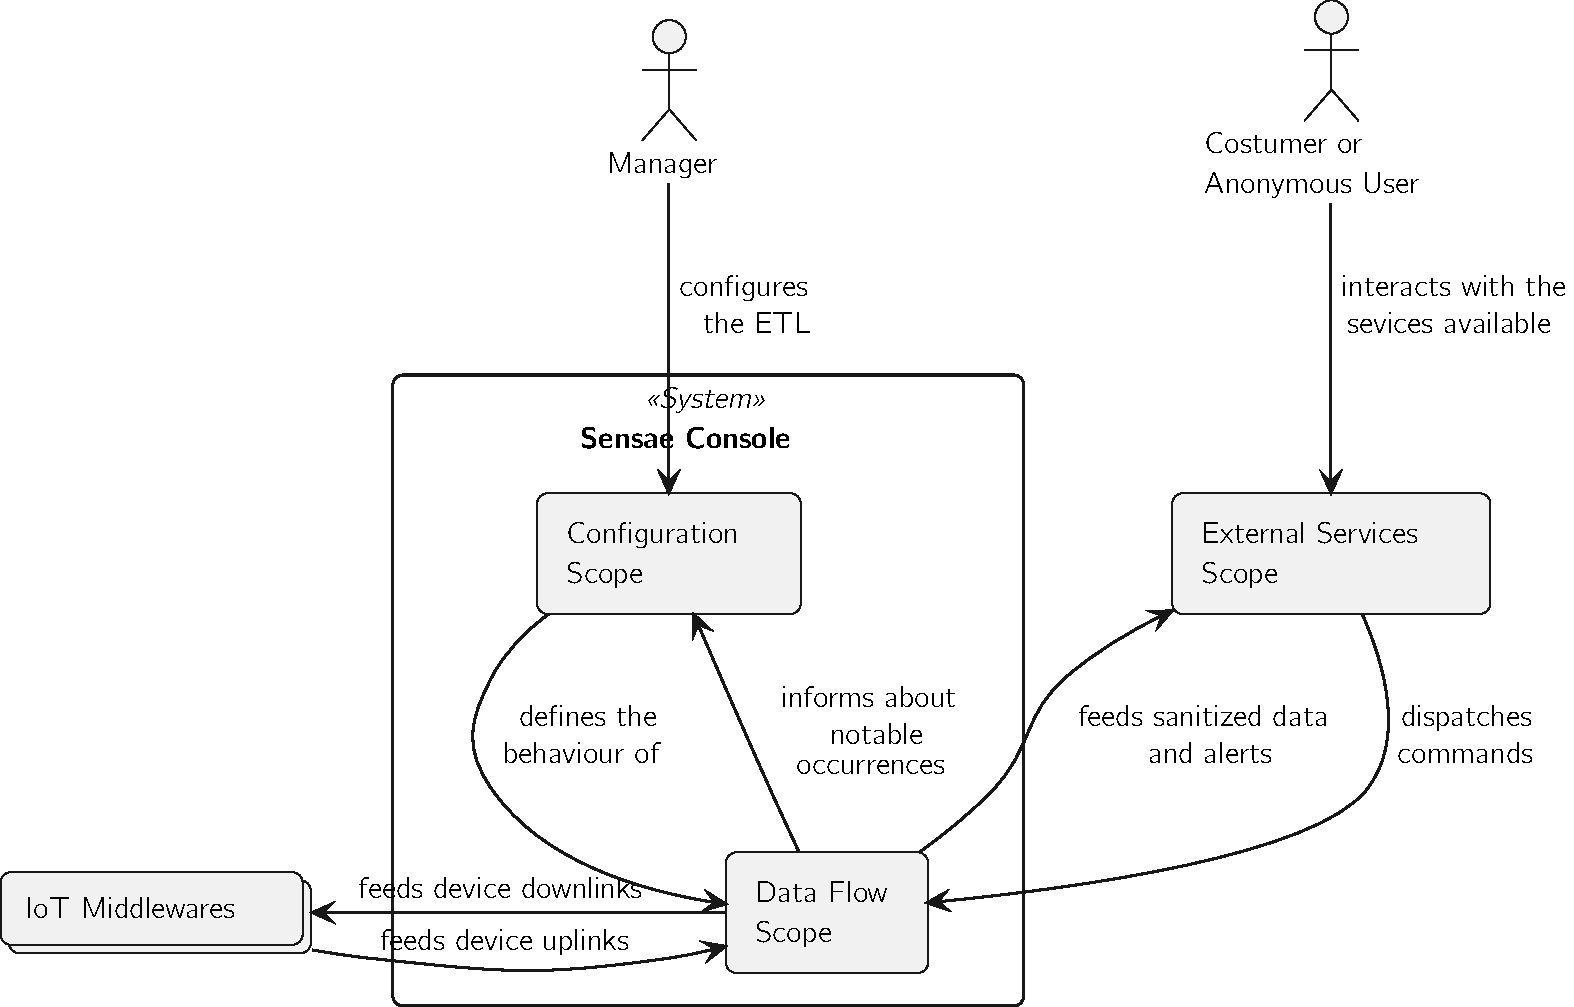
\includegraphics[page=1,width=\columnwidth]{assets/diagrams/design/scopes.pdf}
   \caption[System Scopes]{System Scopes}
   \label{fig:design:system_scopes:scopes}
\end{figure}

The \textbf{Configuration Scope} in Figure~\ref{fig:design:system_scopes:scopes} refers to the configuration and visualization of internal processes/concerns, such as: (i) data decoders, (ii) data mappers (iii) device inventory, (iv) warning rule scenarios definition and (v) device ownership - related to the \textbf{Data Flow Scope}. It is also possible to manage users' access and permissions in the \textbf{Configuration Scope}.

The \textbf{Data Flow Scope} in Figure~\ref{fig:design:system_scopes:scopes} acts as a pipeline where raw data - device uplink - goes through various stages till it is sanitized and ready to be supplied to the \textbf{Business Applications Scope}. The \textbf{Data Flow Scope} is where internal processes occur, such as: (i) data transformation, (ii) data enrichment, (iii) data validation, (iv) data ownership clarification and (v) alert dispatching. It behaves according to what is defined in the \textbf{Configuration Scope}.

The \textbf{Business Applications Scope} in Figure~\ref{fig:design:system_scopes:scopes} is comprised of services that present and act according to the sanitized data and alerts that were supplied to them. These services applicability range from (i) smart irrigation, (ii) fleet management, (iii) fire detection, (iv) physical security access monitoring, (v) air quality monitoring and anything else deemed interesting. The services currently developed are smart irrigation, fleet management and notification management. These will be addressed throughout this and the \nameref{chap:implementation} chapter.

To promote a better understanding of this chapter, the most important terms are described later in the \nameref{subsec:design:domain:taxonomy} Section.

\subsection{Configuration Scope}
\label{subsec:design:system_scopes:configuration_scope}

The \textbf{Configuration Scope} is responsible for managing the following concerns:

\begin{itemize}
   \item \textbf{Data Processor}: manages simple data mappers;
   \item \textbf{Data Decoder}: manages scripts to transform data;
   \item \textbf{Device Management}: manages device information such as name, metadata, static data and other notions;
   \item \textbf{Identity Management}: manages device ownership and users permissions;
   \item \textbf{Rule Management}: manages scripts that consume device data and produce alerts.
\end{itemize}

These concerns can be directly linked to the functional requirements described in the Section related to the~\ref{subsubsec:requirements:functional:sensae:manager} role.

Each concern can be managed by an authorized user, e.g. the data processor concern focus on the creation, deletion and renovation of data mappers.

These operations require various verifications, alter the system internal state and are therefore prolonged.

\subsection{Data Flow Scope}
\label{subsec:design:system_scopes:data_flow_scope}

The \textbf{Data Flow Scope} is responsible for processing incoming data according to what is defined in the \textbf{Configuration Scope}. Both scopes share the same concerns.

This scope also contains four independent units, that aren't controlled by the \textbf{Configuration Scope}:

\begin{itemize}
   \item Data Relayer: responsible for providing a bridge between the \gls{IoT} middlewares and the \textbf{Sensae Console};
   \item Data Gateway: responsible for starting the flow of data in this scope by publishing device uplinks in it;
   \item Data Validator: responsible for filtering device measures based on static rules, e.g. battery percentage reported has to be in between 0 and 100.
   \item Data Store: responsible for persisting data captured in a previously defined state.
\end{itemize}

This scope applies changes to the device measures that flow through the system. These changes are stateless and don't change the overall state of the internal system.

This scope was decoupled from the \textbf{Configuration Scope} even though they both work with the same concerns. The decision was taken based on the pretext that despite the similarities in concerns the operation/business responsibilities of these two scopes were conflicting.

The \textbf{Configuration Scope} requires scarce but heavy computations that alter the internal system state, while the \textbf{Data Flow Scope} requires plentiful but light computations that don't alter the internal system state as summarized in the Table~\ref{tab:design:system_scopes:data_flow_scope:comparison}.

\begin{table}[H]
   \caption[Comparison of Operations in Data Flow and Configuration Scopes]{Comparison of Operations in Data Flow and Configuration Scopes}
   \label{tab:design:system_scopes:data_flow_scope:comparison}
   \centering
   \begin{tabular}{@{}lcc@{}}
   \toprule
   \textbf{Comparison of Operations} & \textbf{Configuration Scope} & \textbf{Data Flow Scope} \\ \midrule
       Alter internal system state & yes & no \\ \hline
       Alter device measures & no & yes \\ \hline
       Required computation power/time & high & low \\ \hline
       Frequency of usage & low & high \\ \hline
   \end{tabular}
\end{table}

Due to this discrepancy it's expected for each scope to have different requirements regarding horizontal scaling. With the addition of more devices to the platform, and subsequently higher ingress volume, \textbf{Data Flow Scope} will need to scale. Since the \textbf{Configuration Scope} is intended mostly for the manager of the platform, a small user pool, the need to scale is smaller.

\subsection{Business Applications Scope}
\label{subsec:design:system_scopes:service_scope}

The \textbf{Business Applications Scope} is responsible for presenting \gls{IoT} business cases to end users. This scope is detached from the \textbf{Sensae Console} due to its dynamic nature. The services that belong to this scope are analogous to plugins.

The scope is comprised of services that consume data and publish commands to \textbf{Data Flow Scope}. Currently, as a \gls{MVP} the implemented business cases are:

\begin{itemize}
   \item \textbf{Fleet Management}: basic service to monitor a fleet of cars regarding their location;
   \item \textbf{Smart Irrigation}: service to automate and monitor the irrigation of zones based on sensor readings;
   \item \textbf{Notification Management}: service to view and manage the delivery of triggered alerts.
\end{itemize}

Each service is bounded to what type of data receives and sends back to the \textbf{Data Flow Scope} as later detailed in the \nameref{subsec:implementation:description:services} Section. The type of data each service handles is enforces by the concepts discussed in Sections~\ref{subsec:design:domain:taxonomy} and \ref{sec:design:domain}. Section~\ref{subsec:design:architecture:solutions} describes these applications architecture with more detail.

Just like plugins, services in this scope are validated and attached to the final deployment by the entity that manages that specific instance. When working in a multi-tenant instance, custom business applications can't be properly verified and therefore their usage is denied.

\subsection{Taxonomy}
\label{subsec:design:domain:taxonomy}

In order for the reader to better understand how the system operates, some concepts need to be better classified and explained:

\begin{itemize}
   \item \textbf{Device}: A device is a "Thing" that can collect data and submit it to \textbf{Sensae Console} via an external system though \textbf{Uplink}s (commonly refereed as a sensor). A device can also receive \textbf{Downlink}s and act base on what was received (commonly refereed as an actuator);
   \item \textbf{Controller}: A controller is a \textbf{Device} that controls and aggregates data from various sub \textbf{Device}s;
   \item \textbf{Records/Metadata}: Records, or Metadata are labels associated to a \textbf{Device} that help an organization to classify and add some information to the owned \textbf{Device}s;
   \item \textbf{Downlink}: A downlink is a term commonly used in radio communications to denote the transmission from the network to the end user. In this case the network is the \textbf{Sensae Console} and the end user is a \textbf{Device};
   \item \textbf{Uplink}: An uplink is the opposite of a \textbf{Downlink}, it's the transmission from a \textbf{Device} to the \textbf{Sensae Console};
   \item \textbf{Data Unit}: A data unit represents the collected measures that are atomically submitted via an \textbf{Uplink} to the \textbf{Sensae Console}. This data should be, at least, enriched with an unique identifier of the \textbf{Uplink} and \textbf{Device} that sent it. The data unit can contain measures captured by various devices, in that case the device is identified as a Controller;
   \item \textbf{Device Command}: A device command is an abstraction on top of a \textbf{Downlink}, intended to instruct a \textbf{Device} to execute a specific action. This devices are commonly identified as actuators. As an example, one could send a command to open or close a valve that is incorporated into a \textbf{Device};
   \item \textbf{Decoder}: A decoder is a function that translates a \textbf{Data Unit} into something that \textbf{Sensae Console} understands;
   \item \textbf{Domain}: A domain represents a department in a organization. An organization is composed of several domains structured in a tree like format;
   \item \textbf{Tenant}: A tenant is a user that belongs to one or more \textbf{Domain}s and represents any of the roles discussed in Section~\ref{sec:requirements:functional};
   \item \textbf{Alert}: A report about a detected condition based on the gather \textbf{Data Unit};
   \item \textbf{Topic}: A Topic is a subcategory of the type of contents that are traded between the various entities of \textbf{Sensae Console} and the \textbf{Business Applications}.
\end{itemize}

Currently the \textbf{Topic}s that flow in the system are:

\begin{itemize}
   \item \textbf{Data}: This topic references the \textbf{Data Unit} concept and is intended to be processed by the \textbf{Data Flow Scope} and consumed by the \textbf{Business Applications};
   \item \textbf{Command}: This topic references the \textbf{Device Command} concept and is intended to be used mainly by the \textbf{Business Applications};
   \item \textbf{Alert}: This topic references the \textbf{Alert} concept and is intended to be consumed mainly by the \textbf{Business Applications};
   \item \textbf{Internal}: This topic references the internal state maintained in the \textbf{Configuration Scope} and \textbf{Data Flow Scope}.
\end{itemize}

These concepts are referenced across the document.

\section{Sensae Console - Architectural Design}
\label{sec:design:architecture}

In order to describe the system in detail at the architectural level, an approach based on the combination of two models, C4 \parencite{c4model-site} and 4+1 \parencite{4plus1model} will be followed.

The 4+1 View Model, proposes the description of the system through complementary views, thus allowing to separately analyze the requirements of various software stakeholders, such as users, system administrators, project managers, architects, and programmers.

The five views are thus defined as follows:
\begin{itemize}
   \item \textbf{Logical view}: relative to the aspects of the software aimed at responding to business challenges;
   \item \textbf{Process view}: relative to the process flow or interactions within the system;
   \item \textbf{Implementation View}: relative to the organization of the software in its development environment;
   \item \textbf{Physical view}: relative to the mapping of the various components of the software in hardware, i.e. where the software is executed;
   \item \textbf{Scenario view}: related to the association of business processes with actors capable of triggering them.
\end{itemize}

The C4 Model advocates for the description of software through four levels of abstraction:
(i) context, (ii) container, (iii) component, (iv) code. Each level adopts a finer granularity than the level that precedes it, thus giving access to more details of a smaller portion of the system.
These levels can be linked to maps, e.g. the context view corresponds to the globe, the container corresponds to the map of each continent, the component view corresponds to the map of each country, and the code view to the map of roads and neighborhoods in each city.

Different levels tell different stories to different audiences.

The levels are defined as follows:

\begin{itemize}
   \item \textbf{Level 1}: Description (context) of the system as a whole;
   \item \textbf{Level 2}: Description of system containers;
   \item \textbf{Level 3}: Description of components of the containers;
   \item \textbf{Level 4}: Description of the code or smaller parts of the components.
\end{itemize}

These two models can be said to expand along distinct axes, with the C4 Model presenting the system with different levels of detail and the 4+1 View Model presenting the system from different perspectives. By combining the two models it becomes possible to represent the system from several perspectives, each with various levels of detail.
To visually model/represent the ideas designed and alternatives considered, the \gls{UML} was used.

In the following sections only combinations of perspectives and levels deemed relevant for the design of the solution are presented.

To better explain the internal communication of \textbf{Sensae Console}, and how the \gls{API} for Business Applications works, the Section~\ref{sec:design:domain} introduces the Canonical Model built to define the protocol for information exchange inside the system. This section does not represent any C4 Level 

The C4 level 4, code, will not be exhibited.

\subsection{C4 Level 1 - Context}
\label{subsec:design:architecture:context}

The context level aims at introducing the system as a whole. The external systems and users that communicate/interact with the system, \textbf{Sensae Console}, and solutions, \textbf{Business Applications} are demonstrated.
\textbf{Business Applications} are briefly introduced here to better explain the reasons behind the architectural decisions taken, they are later discussed in Section~\ref{subsec:design:architecture:solutions}.
Throughout this section the relevant C4 views of level 1 (context level) are presented.

\subsubsection{Context Level - Logical View}
\label{subsubsec:design:architecture:context:logical}

The logical view of the system is introduced here, complete but not detailed, in order to answer the use cases and requirements discussed in Chapter~\ref{chap:requirements}. This takes into account the interactions of \textbf{Sensae Console} and \textbf{Business Applications} with foreign systems and their interactions with the various actors of the system (Figure~\ref{fig:design:architecture:context:logical:diagram}) as required by Section~\ref{subsec:requirements:non_functional:design}.

\begin{figure}[H]
   \centering
   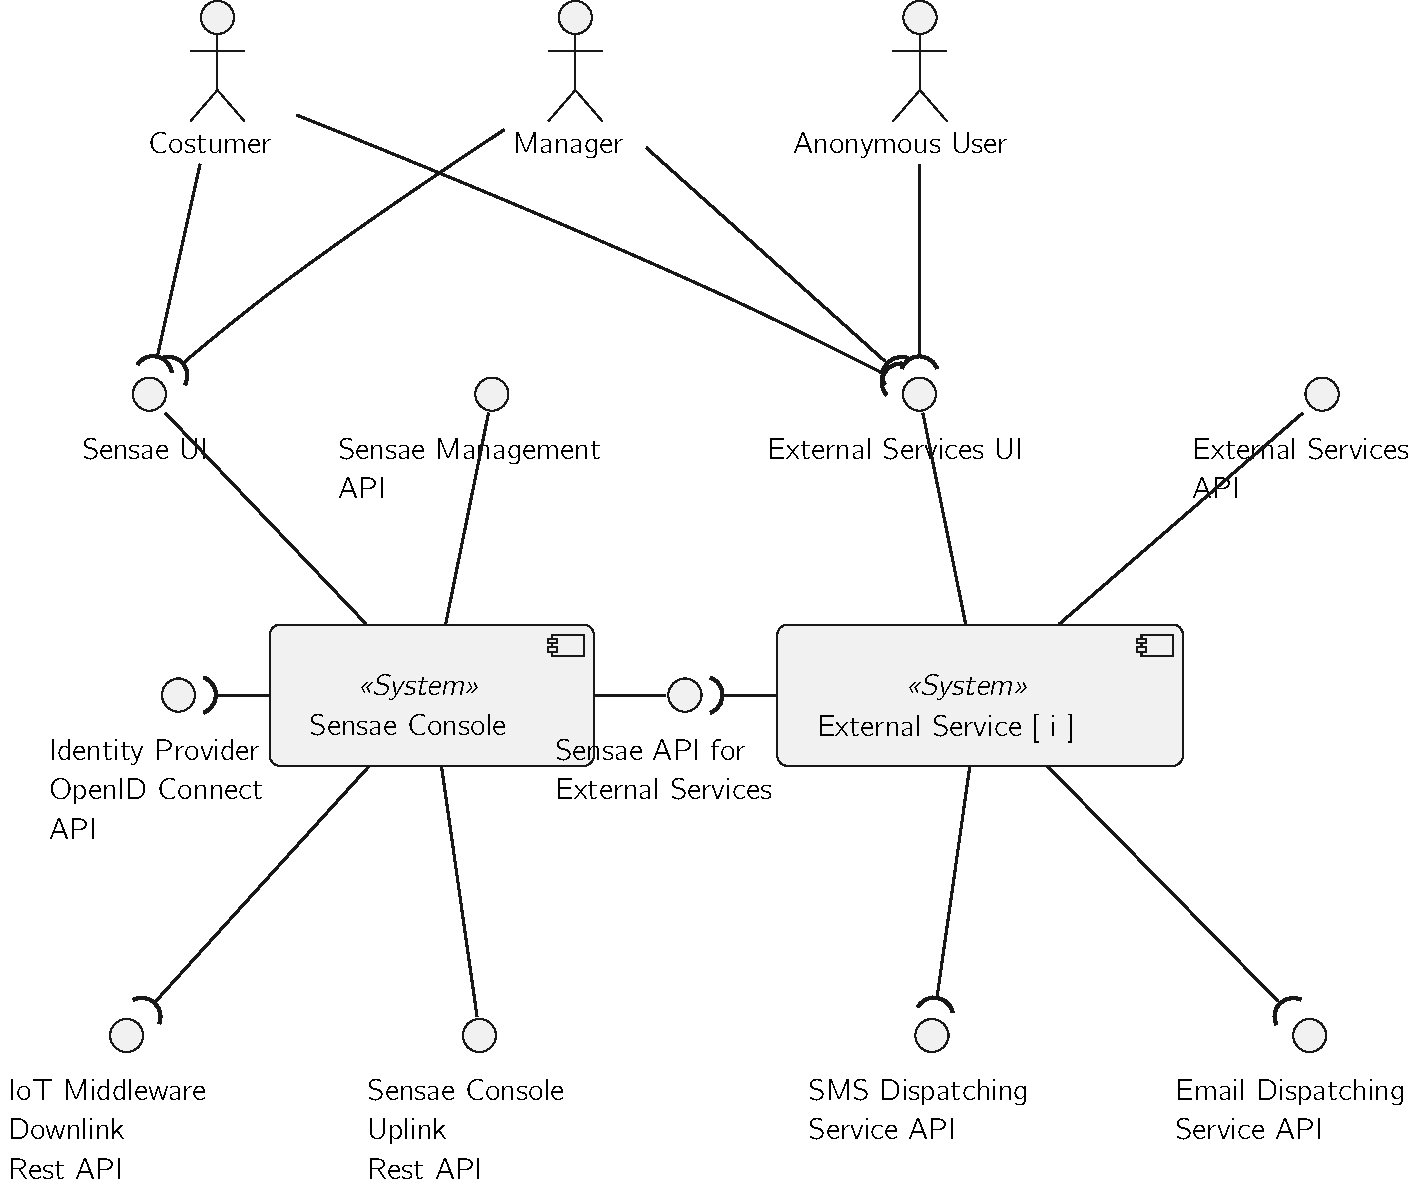
\includegraphics[page=1,width=0.8\columnwidth]{assets/diagrams/design/architectural/level1/logical-view.pdf}
   \caption[Solution - Context Level - Logical View Diagram]{Solution - Context Level - Logical View Diagram}
   \label{fig:design:architecture:context:logical:diagram}
\end{figure}

The \textbf{Business Applications} in Figure~\ref{fig:design:architecture:context:logical:diagram} are represented as an independent collection of systems that consume the \textbf{Sensae Console} \gls{API}. This \gls{API} is responsible for streaming information such as device measures, device commands, alerts and internal state asynchronously. These concept's semantics and structure are enforced by a library, \textit{iot-core}, also developed and discussed in Section~\ref{sec:design:domain}.

All systems provide an \gls{API} for automated management/control and a \gls{UI} for ease of use and data visualization.

As mentioned before in Section~\ref{subsubsec:requirements:functional:services:fire} there is a need to integrate the final product with an Email and SMS dispatch service.

The reason that lead to the use of external authentication/identity services, as required in Section~\ref{subsec:requirements:non_functional:interface}, is further discussed in Appendix~\ref{appendix:design:alternatives:auth}.

\subsubsection{Context Level - Physical View}
\label{subsubsec:design:architecture:context:physical}

Next is the physical view (Figure~\ref{fig:design:architecture:context:physical:diagram}), intended to familiarize the reader with the environment where the solution runs.

\begin{figure}[H]
   \centering
   \begin{subfigure}[b]{0.45\textwidth}
       \centering
       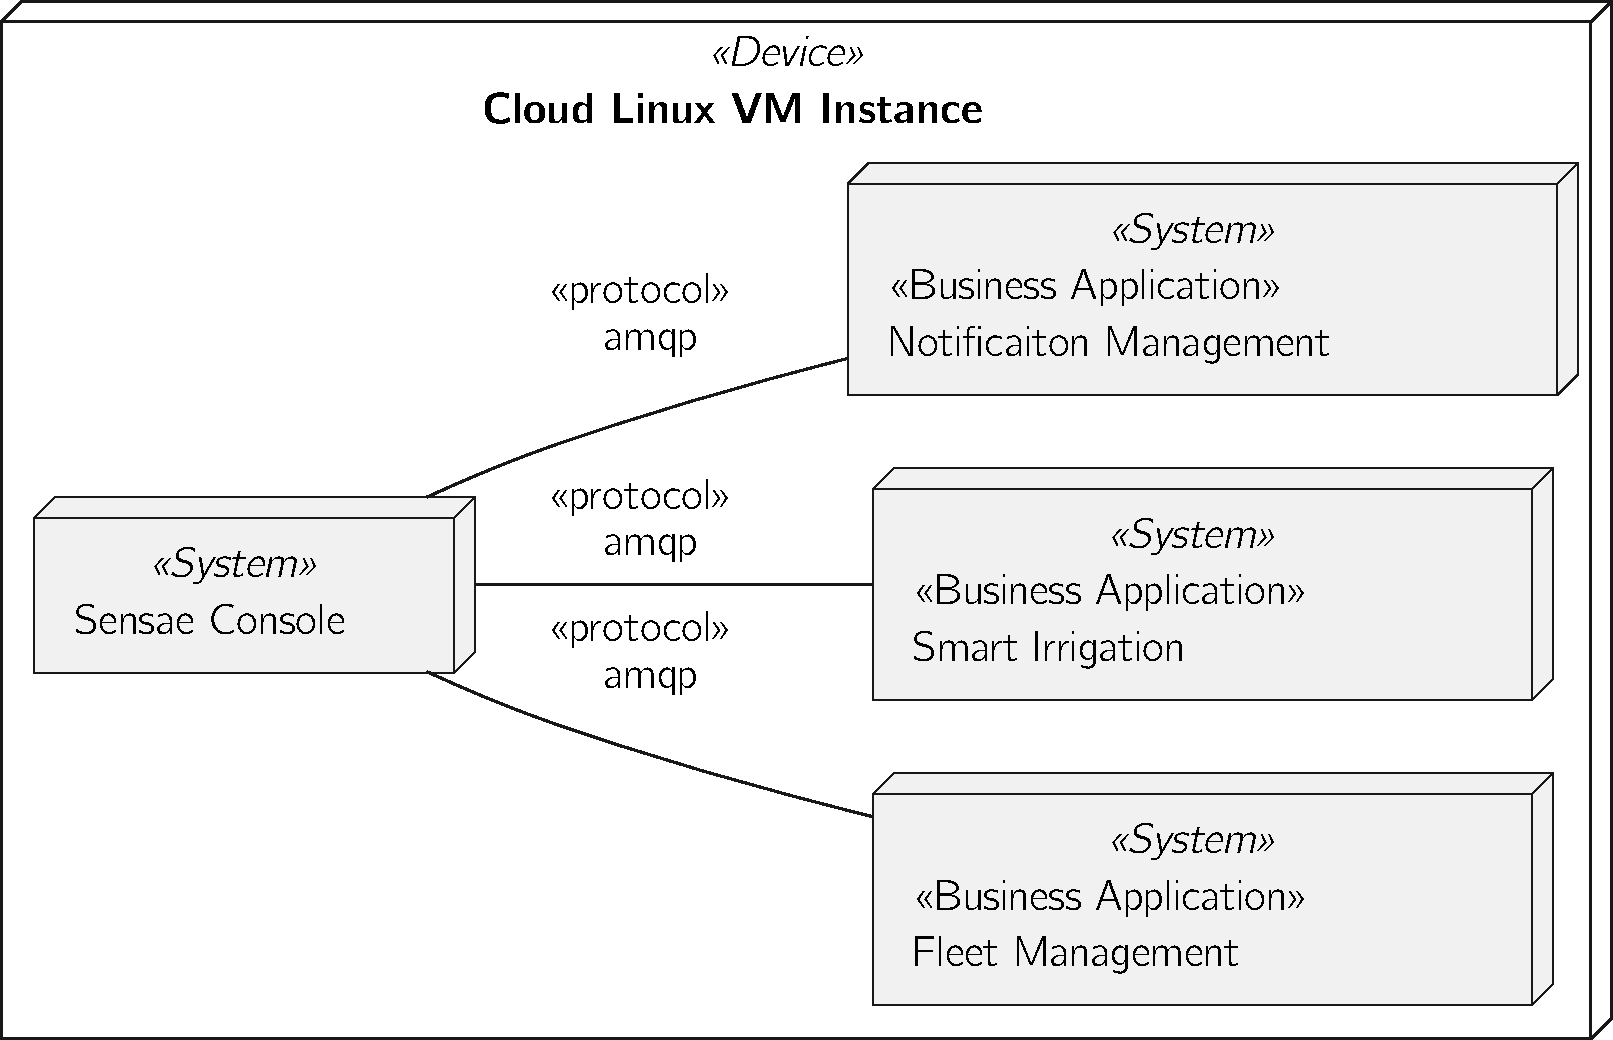
\includegraphics[page=1,width=\columnwidth]{assets/diagrams/design/architectural/level1/physical-view-multi-tenant.pdf}
       \caption{Multi-Tenant\\ Instance}
       \label{fig:design:architecture:context:physical:diagram:multi}
   \end{subfigure}
   \hfill
   \begin{subfigure}[b]{0.45\textwidth}
       \centering
       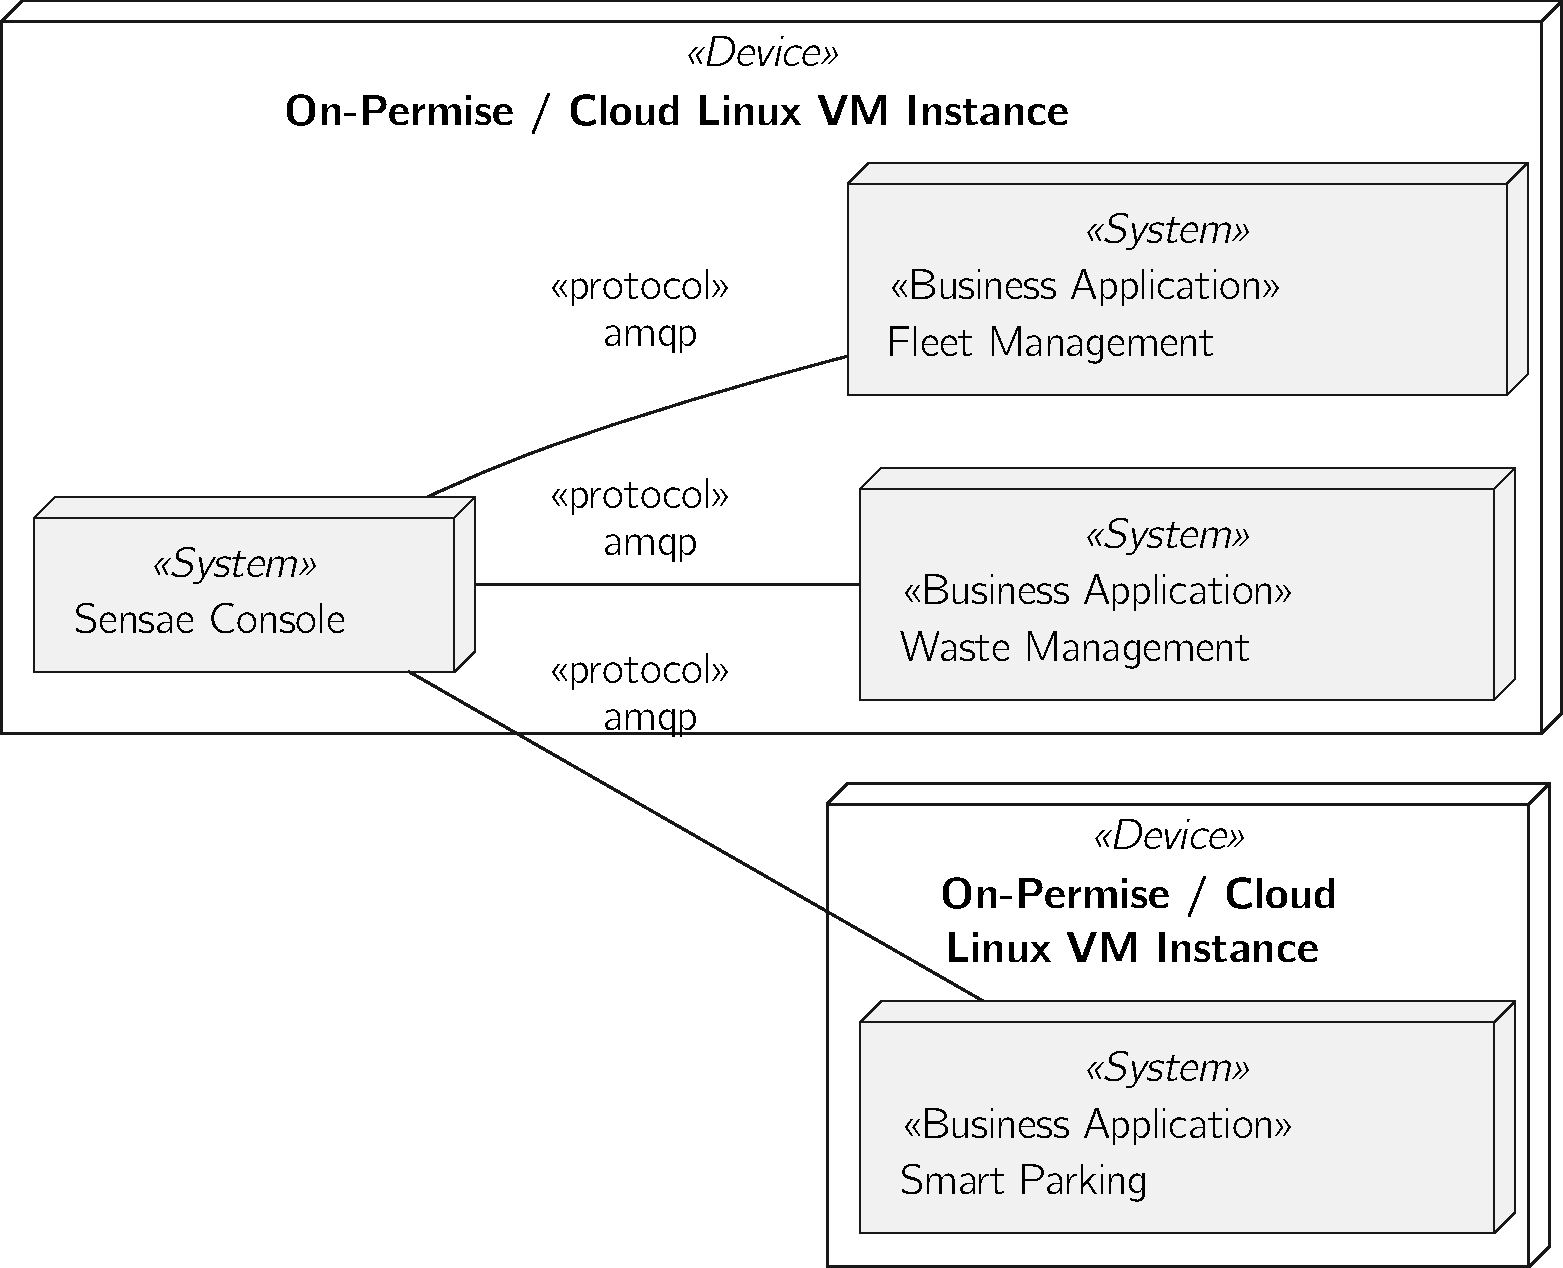
\includegraphics[page=1,width=\columnwidth]{assets/diagrams/design/architectural/level1/physical-view-single-tenant.pdf}
       \caption{Single-Tenant\\ Instance}
       \label{fig:design:architecture:context:physical:diagram:single}
   \end{subfigure}
      \caption[Solution - Context Level - Physical View Diagrams]{Solution - Context Level - Physical View Diagrams}
      \label{fig:design:architecture:context:physical:diagram}
\end{figure}

There are two major options when deploying a new \textbf{Sensae Console}: (i) cloud and (ii) on-premise deployment.
Each deployment can be a:

\begin{itemize}
   \item Multi-Tenant Instance (Figure~\ref{fig:design:architecture:context:physical:diagram:multi}): This deployment serves various costumers and therefore, all business applications are developed and validated by the company to avoid interacting with services that may abuse the system in nefarious ways. Currently, for this type of instance, the Sensae Console and the Business Applications run in a single instance. The business applications correspond to the developed \gls{PoC}s.
   \item Single-Tenant Instance (Figure~\ref{fig:design:architecture:context:physical:diagram:single}): This deployment serves a single costumer, therefore he/she can connect custom business applications that aren't validated or developed by the company. The two custom business applications serve as an example of the freedom given to the costumer to interact with the system. 
\end{itemize}

The connections to external systems and interactions with users were hidden for brevity reasons. The reason for these distinct deployment options derive from the discussion in Chapter~\ref{chap:requirements}.  

\subsubsection{Context Level - Synopsis}
\label{subsubsec:design:architecture:context:synopsis}

The context level introduces the reader to the bigger picture of the whole solution, but it contains little to no information about how the system functions internally.

The process view was not represented since at this level the interactions between the system, actors and external systems, are too abstract to be relevant for the reader.
The implementation view was also not represented since the \textbf{Sensae Console} and \textbf{Business Applications} were developed as a single project.

The Section~\nameref{subsec:design:architecture:platform} will dive into the internals of the \textbf{Sensae Console}.
The solutions developed are later discussed in Section~\ref{subsec:design:architecture:solutions}.

\subsection{C4 Level 2 - Container}
\label{subsec:design:architecture:platform}

This section will explore the internals of \textbf{Sensae Console} from an architectural point of view. It mainly discusses the C4 container level.
The C4 Level 3 - Component is discussed in Appendix~\ref{appendix:design:architecture:platform:components}.

The C4 level 2 presents the various containers that compose the platform. In this section all relevant views will be presented according to the alternative in use or idealized for the system. In the Section~\ref{sec:design:alternatives} other alternatives are discussed.

The description of this level of abstraction begins with the logical view.

\subsubsection{Container Level - Logical View}
\label{par:design:architecture:platform:container:logical}

In order to support the functional requirements identified (Section~\ref{sec:requirements:functional}), and knowing that \textbf{Sensae Console} will serve multiple users with different levels of access to the managed information, the various business concepts were segregated from the user interaction. The configuration management also had to be separated from the data pipeline, knowing that \textbf{Sensae Console} will process a high volume of device measures.

Considering the need to persist and provide the information collected, the system integrates databases, which are not developed, but only configured and operated - using a \gls{DBMS}.

The system also uses one (or more) message brokers, \cite{broker}, that will be configured but not developed.

In order to ease the analysis of the platform, the following diagram (Figure~\ref{fig:design:architecture:platform:containers:logical:complete}) presents a complete view of \textbf{Sensae Console} where each concern represents a group of containers. These groups are then explored in detail.

As seen in the diagram:

\begin{itemize}
   \item Each concern exposes a \gls{UI} and an \gls{API}, these are aggregated in the \textbf{UI Aggregator} container that then exposes everything as a single \gls{UI} and \gls{API} for management;
   \item The Device Management concern consumes the \gls{IoT} Middleware API since it is responsible for sending downlinks to devices;
   \item The Message Broker exposes an \gls{API}, this is the \gls{API} that the \textbf{Business Applications} consume to access the information that flow in \textbf{Sensae Console};
   \item The Identity Management concern consumes the Identity Provider's OpenID Connect API to handle User Authentication;
   \item The Message Broker is responsible for routing messages through the system and ensuring that the various containers communicate;
   \item The Data Store Backend and Data Store Database are responsible for storing data in a specific format, defined at startup via configuration;
   \item The Data Relayer and Data Gateway are responsible for exposing an \gls{API} for data ingestion and publish the ingested data in the system through the Message Broker;
   \item The Data Validator applies simple filters to incoming data, for example, measures that report a soil moisture of 120\% are marked as incorrect.
\end{itemize}

\begin{sidewaysfigure}
   \centering
   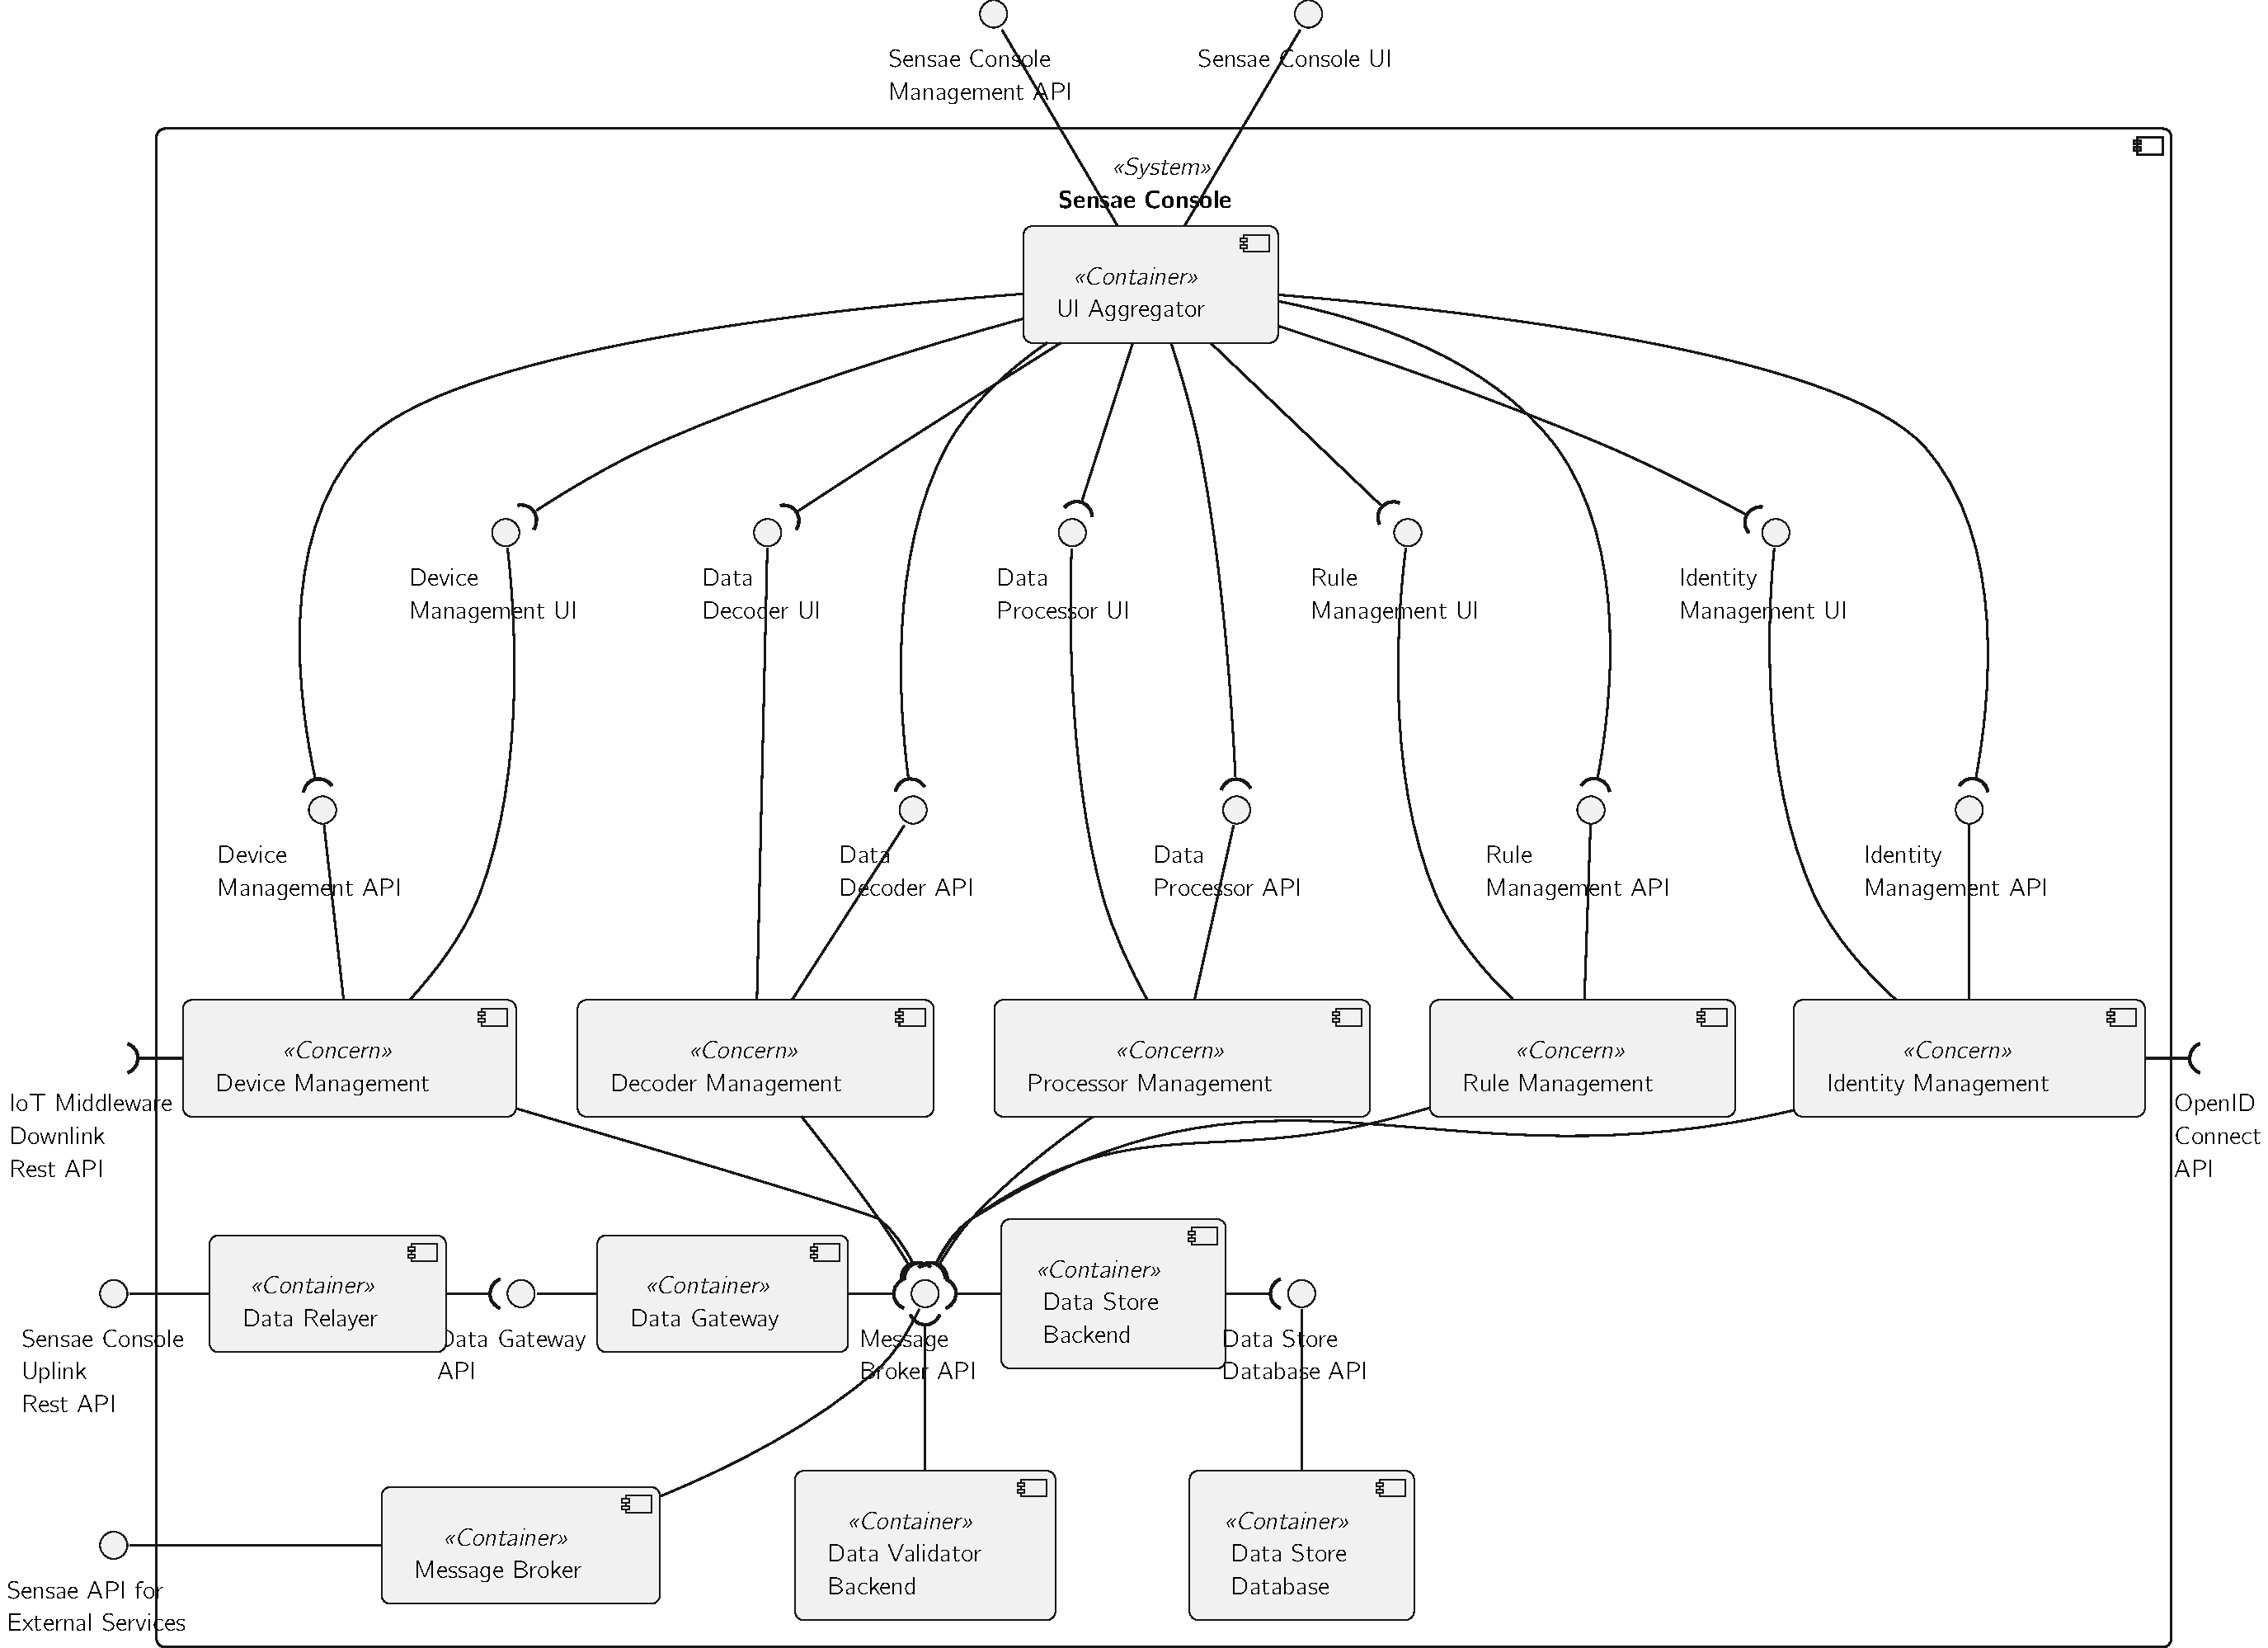
\includegraphics[page=1,width=0.8\columnwidth]{assets/diagrams/design/architectural/level2/logical/contexts-v2.pdf}
   \caption[Sensae Console - Container Level - Logical View Diagram]{Sensae Console - Container Level - Logical View Diagram}
      \label{fig:design:architecture:platform:containers:logical:complete}
\end{sidewaysfigure}

Each concern in Figure~\ref{fig:design:architecture:platform:containers:logical:complete} is composed by containers that belong to the \textbf{Configuration} and \textbf{Data Flow} Scopes (represented in yellow in the following diagrams).
The Configuration Scope of each concern is composed by a three layers architecture, as per \cite{3tier}:

\begin{itemize}
   \item \textbf{Presentation Layer}: the user interface and communication layer of the application where the user interacts with the system;
   \item \textbf{Application Layer}: the business layer of the application where information from the \textbf{Presentation Layer} is processed and sent to the \textbf{Data Layer};
   \item \textbf{Data Layer}: the infrastructure layer of the application where data is stored and requested as needed.
\end{itemize}

The Data Flow Scope is usually composed by a single container that only consumes the Message Broker \gls{API}.

As a brief description of some of the similar characteristics of all concerns:

\begin{itemize}
   \item The frontend container corresponds to the \textbf{Presentation Layer} and exposes an \gls{UI};
   \item The backend container corresponds to the \textbf{Application Layer} and communicates with the Data Flow container(s) exclusively through the \textbf{Message Broker}. The Backend publishes issues related to the concern's configuration that the Data Flow Container consumes. The Data Flow container publishes metrics related to what resources are being used that are then consumed by the Backend;
   \item The communication exchanged between Backend and Data Flow containers is parameterized according to the Section~\ref{subsubsec:design:domain:shared_model:routing} and is preformed in the Internal Topic;
   \item The backend container exposes an \gls{API} that is consumed by the frontend and optionally by properly authenticated external systems;
   \item The database container corresponds to the \textbf{Data Layer}.
\end{itemize}

The Data Processor concern group is presented in Figure~\ref{fig:design:architecture:platform:containers:logical:processor}.

\begin{figure}[H]
   \centering
   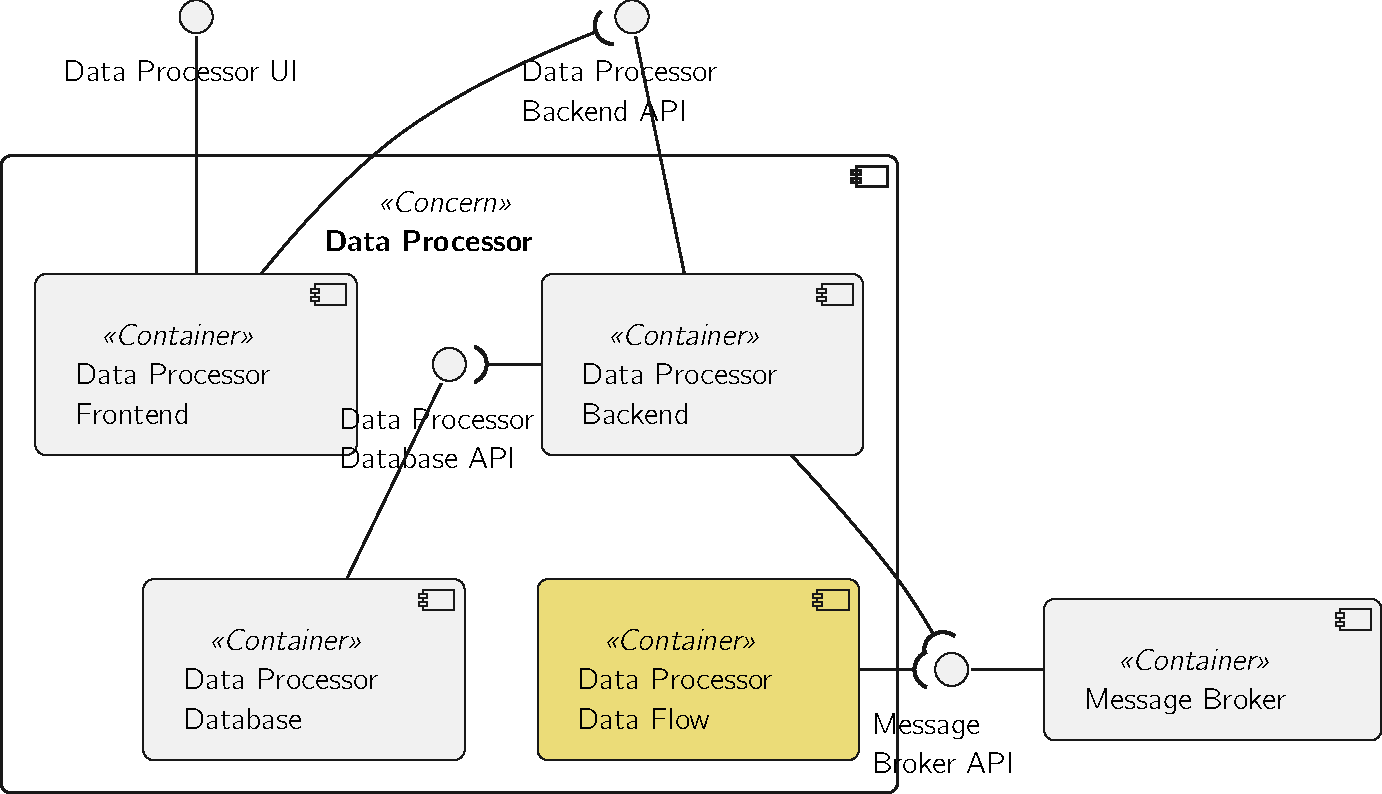
\includegraphics[page=1,width=0.8\columnwidth]{assets/diagrams/design/architectural/level2/logical/data-processor-context.pdf}
   \caption[Data Processor - Container Level - Logical View Diagram]{Data Processor - Container Level - Logical View Diagram}
   \label{fig:design:architecture:platform:containers:logical:processor}
\end{figure}

The concern represented in Figure~\ref{fig:design:architecture:platform:containers:logical:processor} is responsible for transforming the data received in a format and semantic that can be understood by the system, it is explored in detail in Section~\ref{subsubsec:design:domain:bounded_contexts:processor}. The Data Processor Data Flow publishes metrics to the Message Broker regarding the time each Data Processor was used so that the Backend can then report this usages.

The Data Decoder concern group is presented in Figure~\ref{fig:design:architecture:platform:containers:logical:decoder}.

\begin{figure}[H]
   \centering
   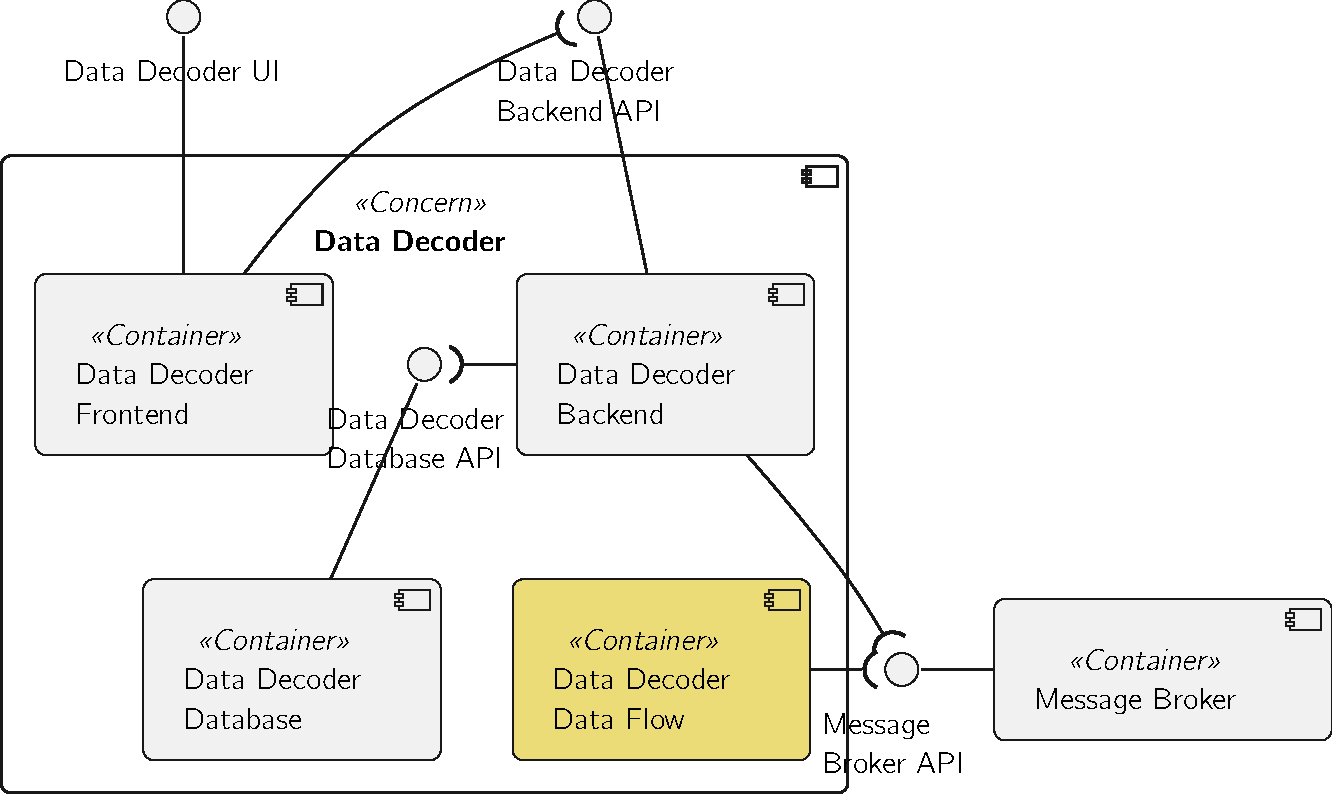
\includegraphics[page=1,width=0.8\columnwidth]{assets/diagrams/design/architectural/level2/logical/data-decoder-context.pdf}
   \caption[Data Decoder - Container Level - Logical View Diagram]{Data Decoder - Container Level - Logical View Diagram}
   \label{fig:design:architecture:platform:containers:logical:decoder}
\end{figure}

The concern represented in Figure~\ref{fig:design:architecture:platform:containers:logical:decoder} is also responsible for transforming the data received in a format and semantic that can be understood by the system. In contrast with the Data Processor, it provides a more flexible but complex way of manipulating data, it is explored in detail in Section~\ref{subsubsec:design:domain:bounded_contexts:decoder}. The Data Decoder Data Flow publishes metrics to the Message Broker regarding the time each Data Decoder was used so that the Backend can then report this usages.

The Device Management concern group is presented in Figure~\ref{fig:design:architecture:platform:containers:logical:device}.

\begin{figure}[H]
   \centering
   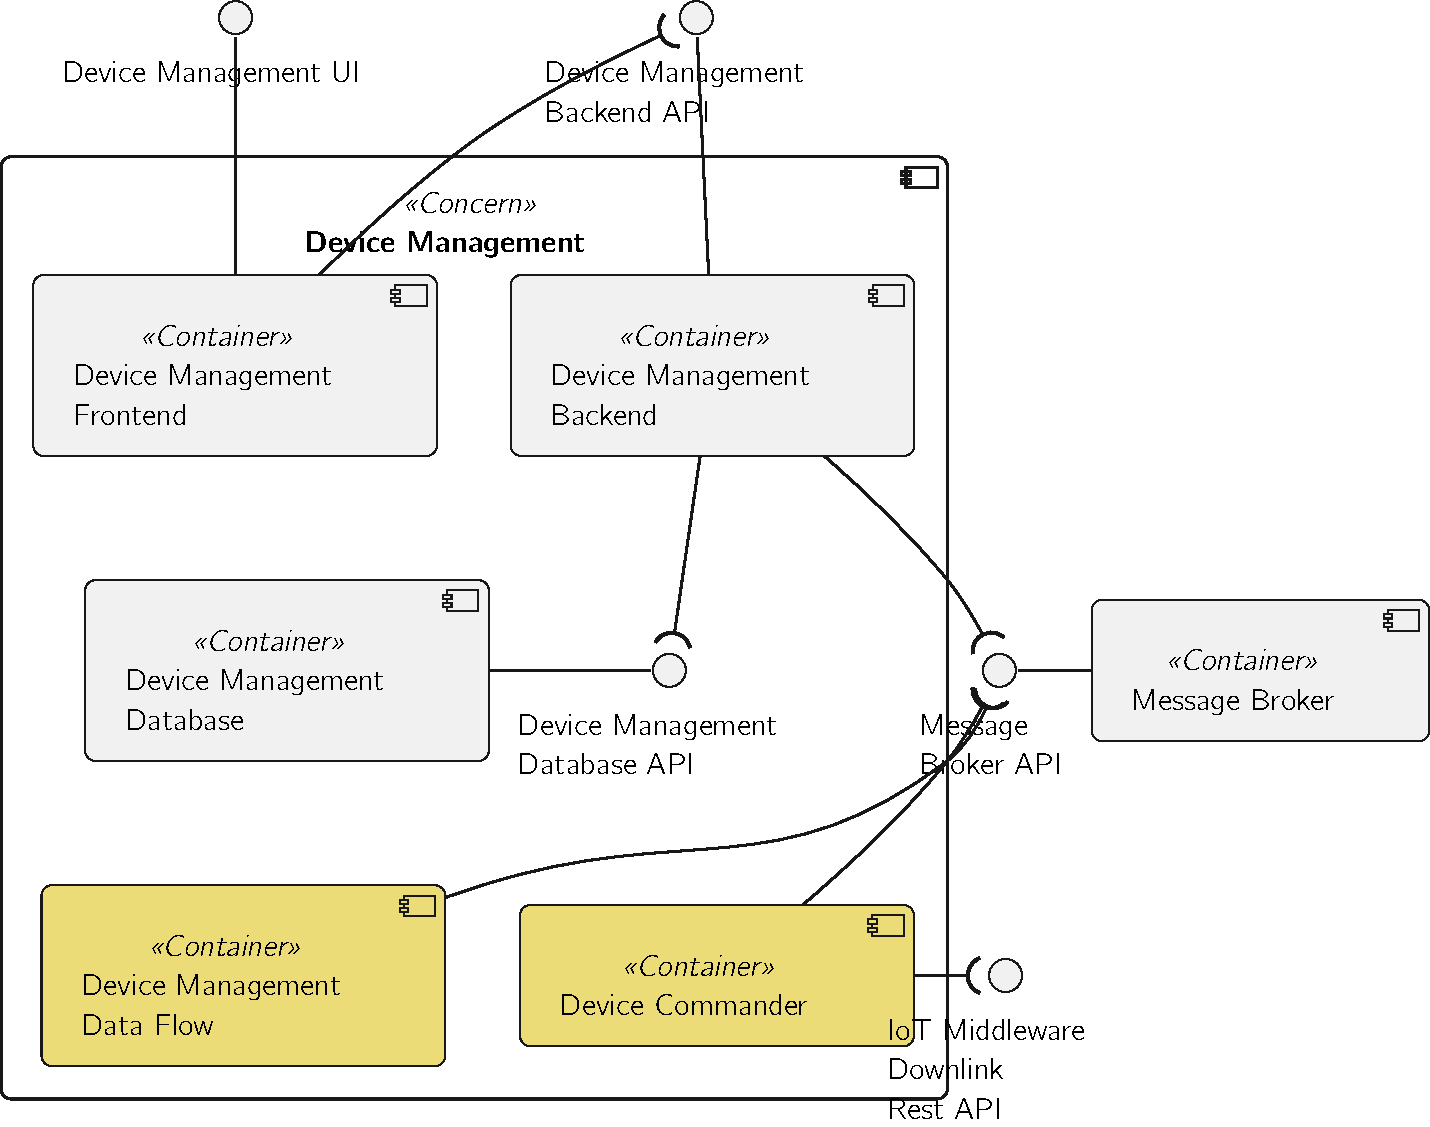
\includegraphics[page=1,width=0.8\columnwidth]{assets/diagrams/design/architectural/level2/logical/device-management-context.pdf}
   \caption[Device Management - Container Level - Logical View Diagram]{Device Management - Container Level - Logical View Diagram}
   \label{fig:design:architecture:platform:containers:logical:device}
\end{figure}

The concern represented in Figure~\ref{fig:design:architecture:platform:containers:logical:device} is responsible for maintaining a registry of the devices in use by the platform.

The Device Management Data Flow enriches the measures collected with more information regarding the device that sent them. The Device Commander consumes an \gls{IoT} Middleware REST \gls{API} to dispatch downlinks to devices. This downlinks contain commands that control the behavior of the implied actuator.
This concern is explored in Section~\ref{subsubsec:design:domain:bounded_contexts:device}. The Data Flow containers publishes metrics to the Message Broker regarding the time each device was used so that the Backend can then report this usages.

The Identity Management concern group is presented in Figure~\ref{fig:design:architecture:platform:containers:logical:identity}.

\begin{figure}[H]
   \centering
   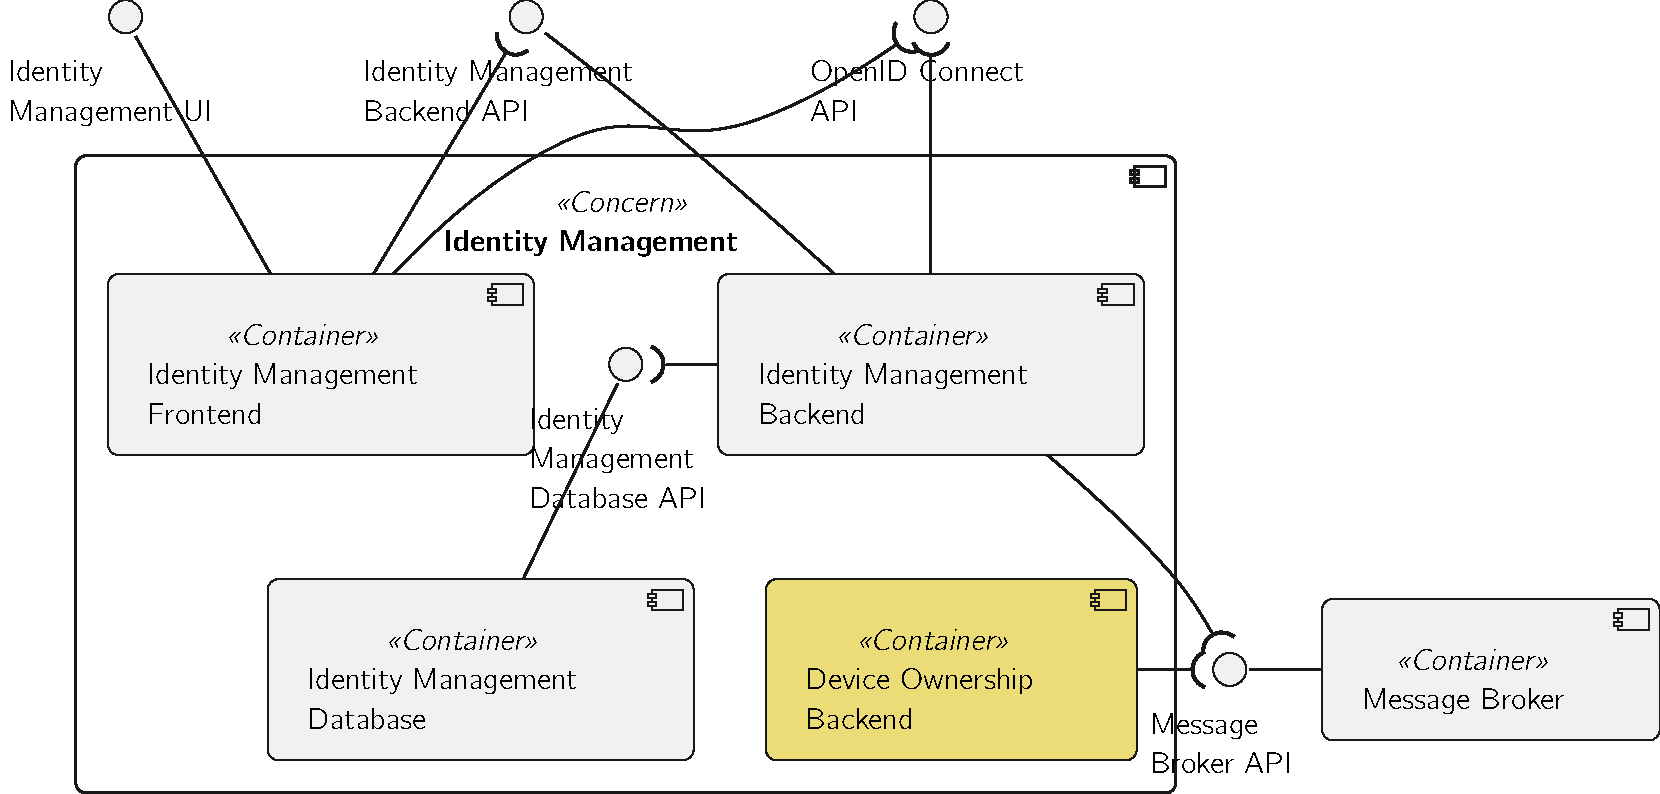
\includegraphics[page=1,width=0.9\columnwidth]{assets/diagrams/design/architectural/level2/logical/identity-management-context.pdf}
   \caption[Identity Management - Container Level - Logical View Diagram]{Identity Management - Container Level - Logical View Diagram}
   \label{fig:design:architecture:platform:containers:logical:identity}
\end{figure}

The concern represented in Figure~\ref{fig:design:architecture:platform:containers:logical:identity} is responsible for managing devices ownership, user identity and organization's details. The backend and frontend containers communicate with an identity provider via OpenID Connect to verify the user identity. The Device Ownership Backend enriches the data measures and alerts with information regarding the organizations that own the device responsible for sending the measures or that lead to the dispatch of an alert. This concern is explored in Section~\ref{subsubsec:design:domain:bounded_contexts:identity}. This data flow container publishes metrics to the Message Broker regarding the time each organization information was used.

The Rule Management concern group is presented in Figure~\ref{fig:design:architecture:platform:containers:logical:rule}.

\begin{figure}[H]
   \centering
   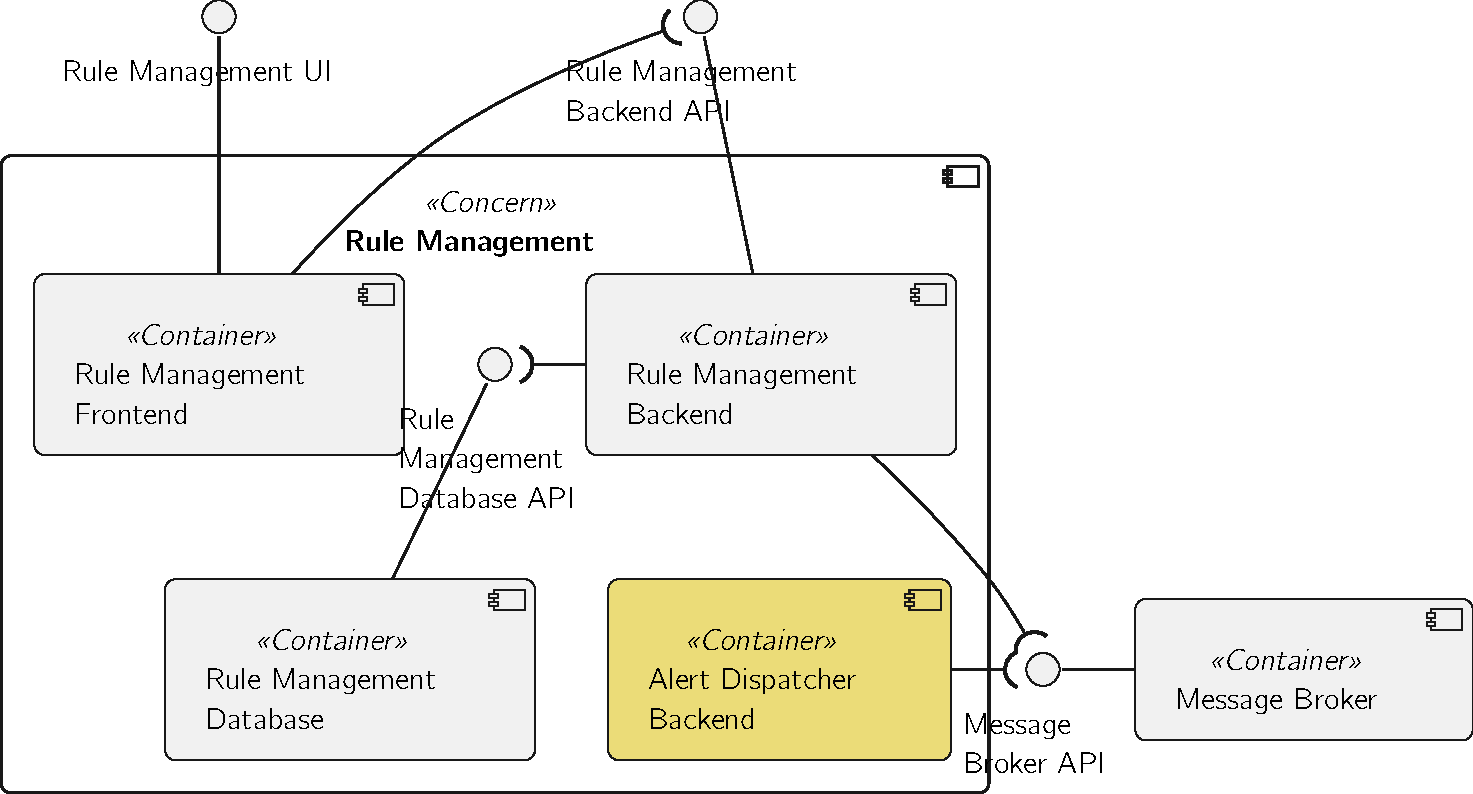
\includegraphics[page=1,width=0.8\columnwidth]{assets/diagrams/design/architectural/level2/logical/rule-management-context.pdf}
   \caption[Rule Management - Container Level - Logical View Diagram]{Rule Management - Container Level - Logical View Diagram}
   \label{fig:design:architecture:platform:containers:logical:rule}
\end{figure}

The concern represented in Figure~\ref{fig:design:architecture:platform:containers:logical:rule} is responsible for managing rule scenarios that produce alerts based on the captured device measures.

The Alert Dispatcher is responsible for publishing alerts based on the rule scenarios published by the Rule Management Backend. The Rule Management Backend ensures that the rules submitted are valid. This concern is explored in Section~\ref{subsubsec:design:domain:bounded_contexts:rule}. This data flow container does not publishes any metrics, its interactions are better described with the help of sequence diagrams available in Figures~\ref{fig:design:architecture:platform:container:process:diagram:init} and \ref{fig:design:architecture:platform:component:process:diagram:rule}.

As the diagrams above presented, all communication between backend containers of both scopes is guaranteed by the Message Broker. This Message Broker exposes its \gls{API} so that Business Applications can consume all information and act according to it. The Section~\ref{subsec:design:architecture:solutions} explores the solutions developed.

In the following section the internal communication of the system is clarified.

\subsubsection{Container Level - Process View}
\label{par:design:architecture:platform:container:process}

In this section, several use cases (according to some functional requirements identified in Section~\ref{sec:requirements:functional}) are presented through sequence diagrams, in order to introduce the reader to the interactions that occur between the various containers of the \textbf{Sensae Console}.

The routing keys used for communication between backend containers can be extrapolated from the model described in the Section~\ref{subsubsec:design:domain:shared_model:routing}.

This section is composed by five sets of important functionalities to discuss at this level of abstraction: (i) system/container initialization (ii) data pipeline operation, (iii) data pipeline configuration, (iv) user authentication/authorization, (v) service usage.

The system/container initialization, presented in Figure~\ref{fig:design:architecture:platform:container:process:diagram:init}, refers to the interval of time since a container is launched till it is ready to process requests or events.

\begin{figure}[H]
   \centering
   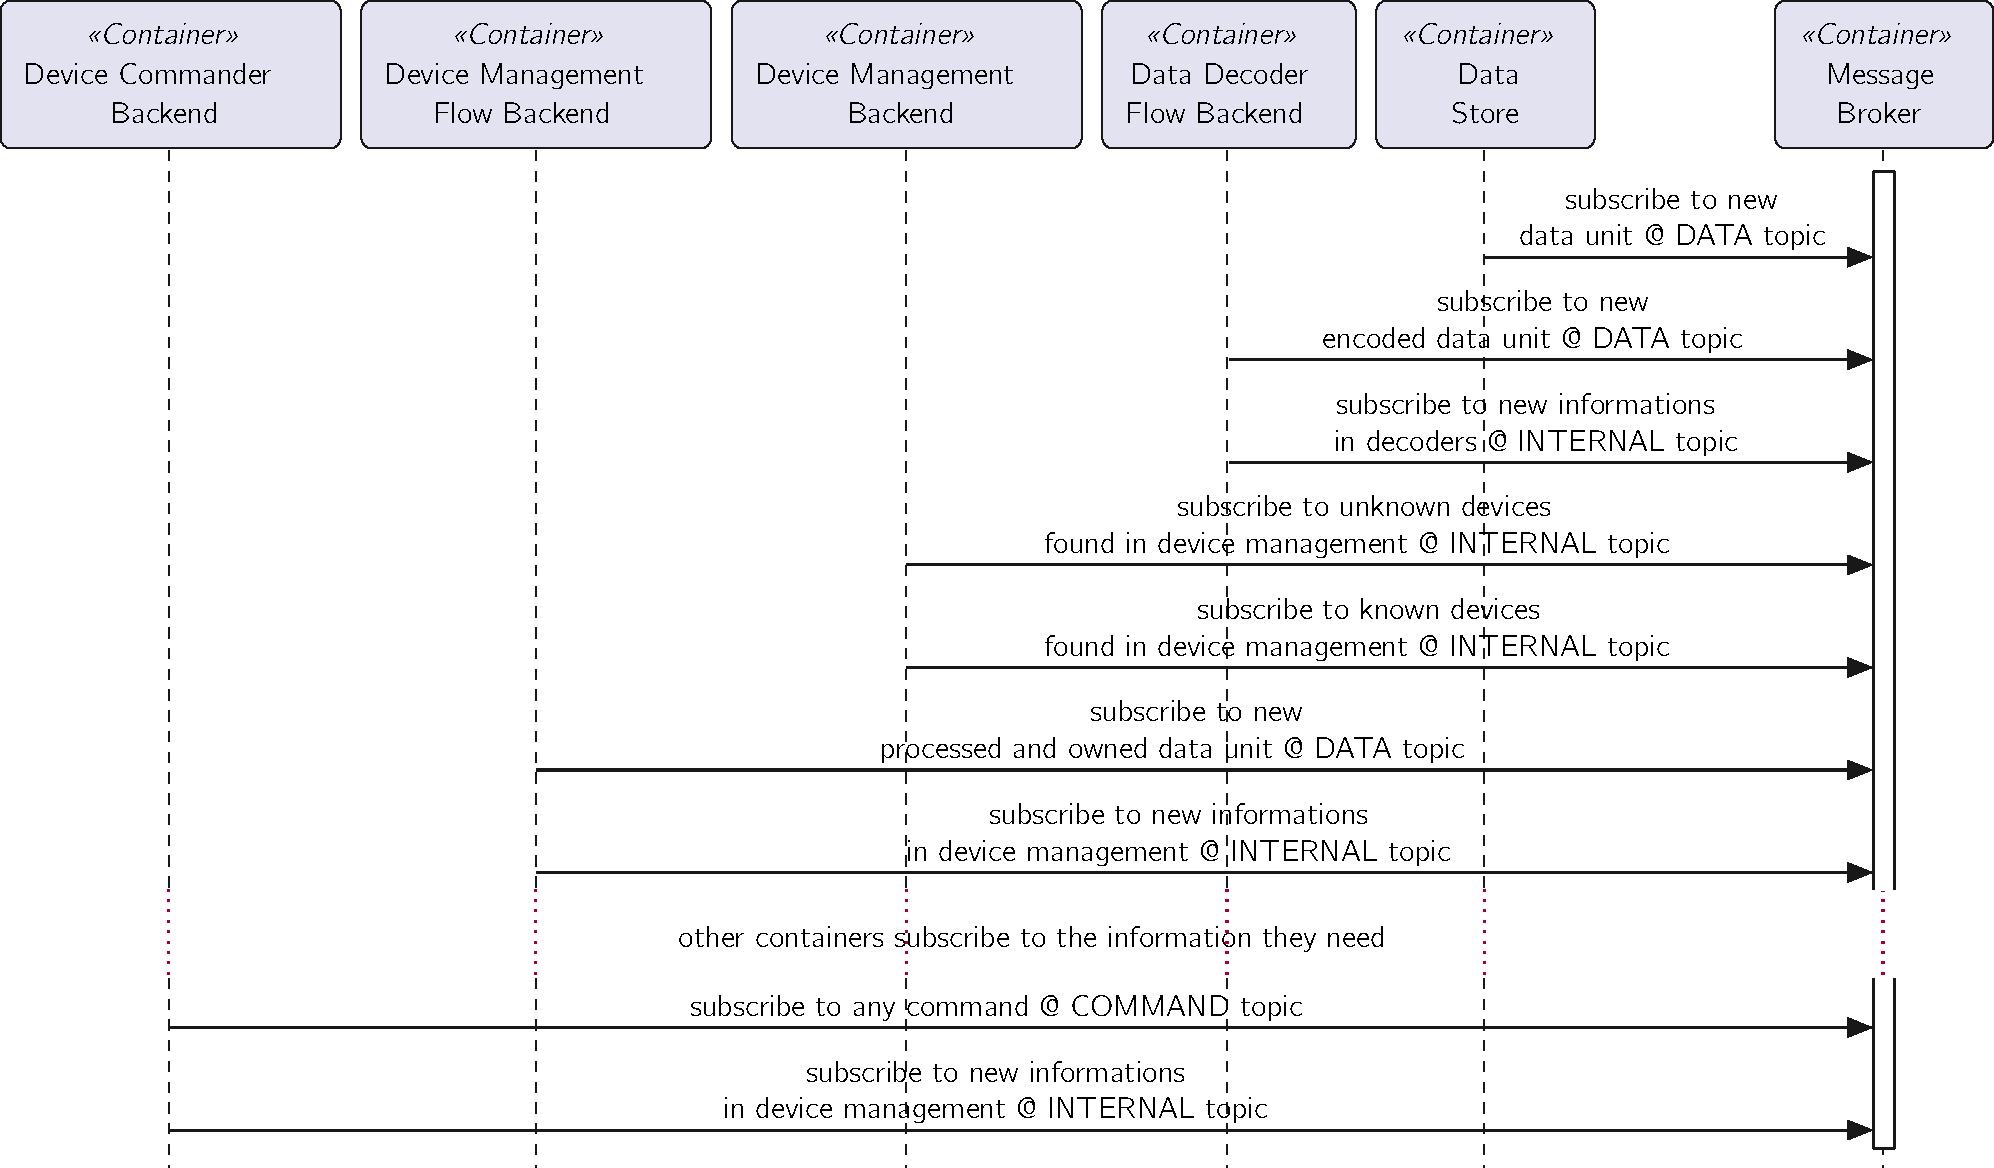
\includegraphics[page=1,width=\columnwidth]{assets/diagrams/design/architectural/level2/process/container-init.pdf}
   \caption[System/Container Initialization - Part 1 - Container Level - Process View Diagram]{System/Container Initialization - Part 1 - Container Level - Process View Diagram}
   \label{fig:design:architecture:platform:container:process:diagram:init}
\end{figure}

Not all containers are displayed in the diagram - Figure~\ref{fig:design:architecture:platform:container:process:diagram:init} - for brevity reasons.
The system relies heavily in the Pub/Sub \parencite{pubsub} pattern to communicate internally via a message broker. In this scenario the first step in a container life cycle is to subscribe to the information that it needs as presented in the diagram above.

Certain containers need the entire state related to their concern to function. So, after subscribing to the needed information, they notify the system that they have entered an \textit{init state} for a specific concern. This triggers the creation of new events to help that container to reach a \textit{ready state}. An example of this interaction is presented in the following diagram, Figure~\ref{fig:design:architecture:platform:container:process:diagram:ready}.

\begin{figure}[H]
   \centering
   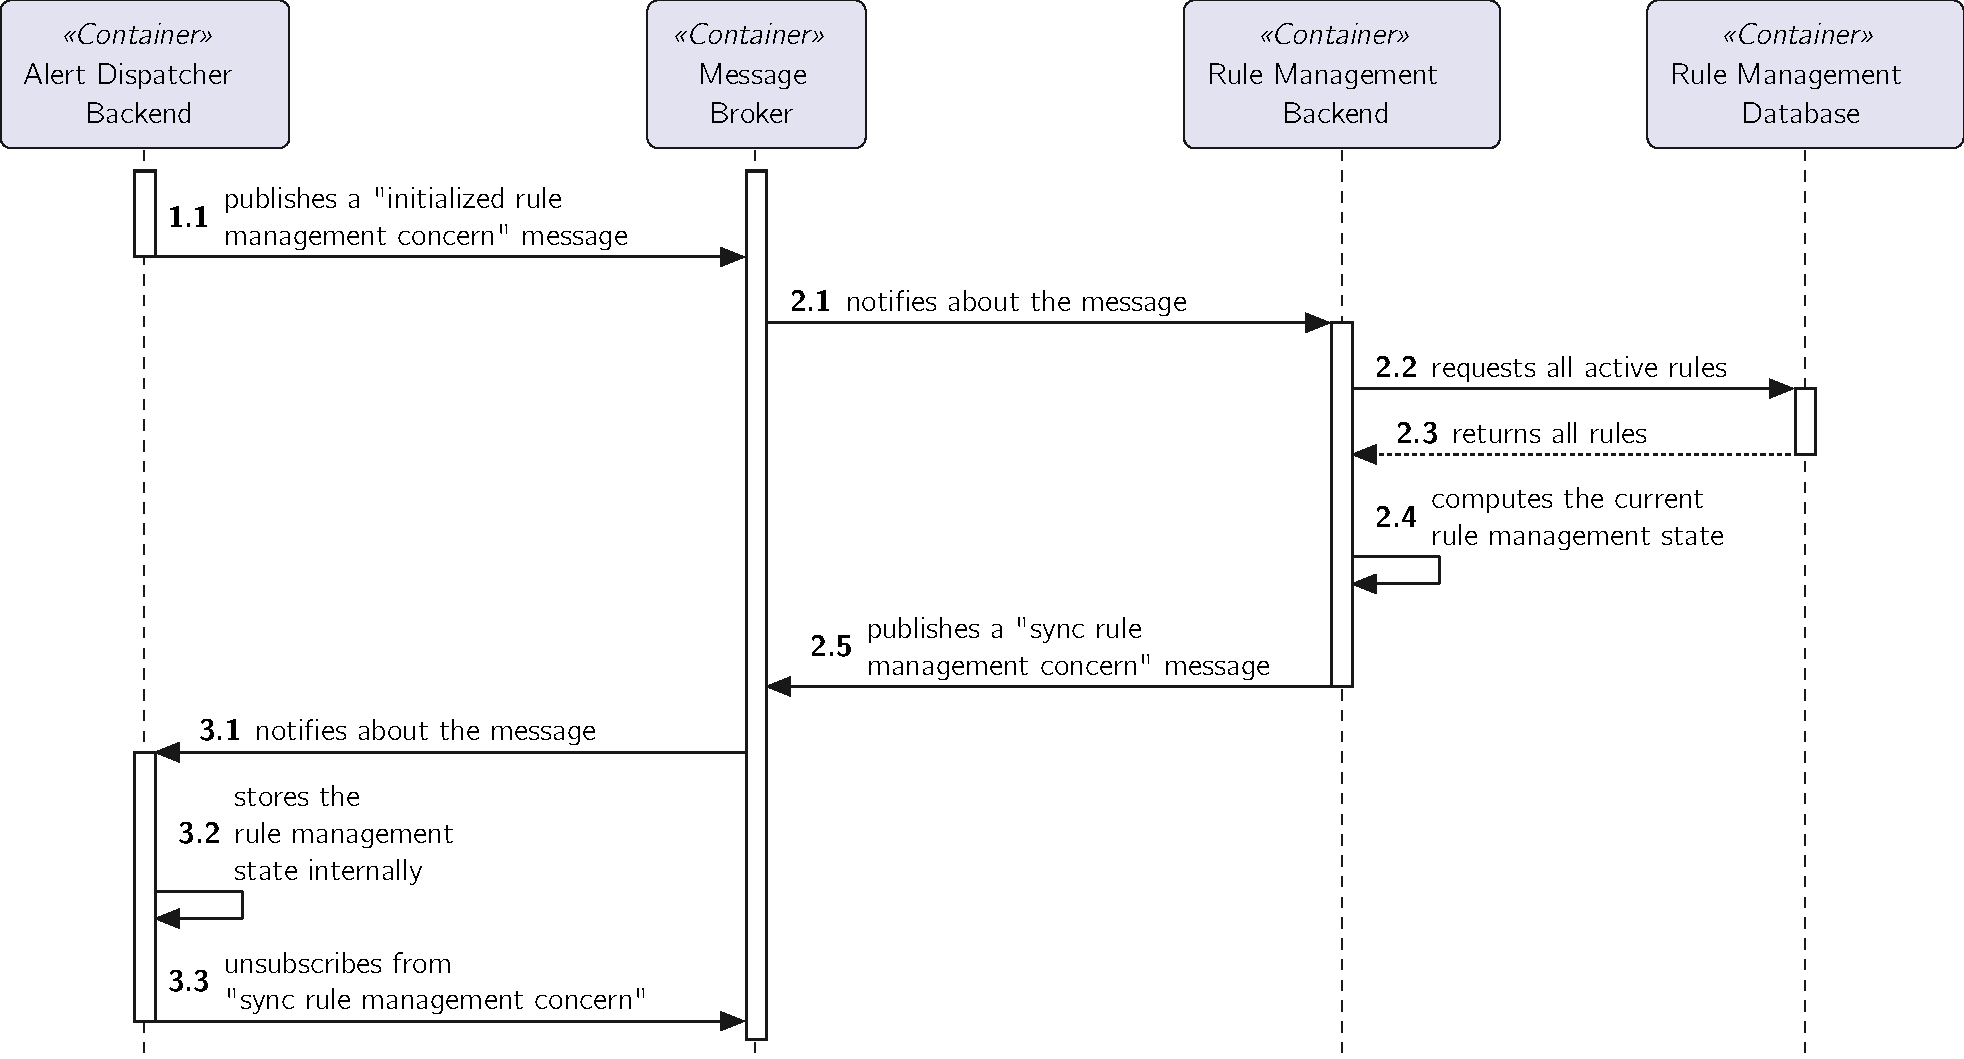
\includegraphics[page=1,width=\columnwidth]{assets/diagrams/design/architectural/level2/process/container-ready.pdf}
   \caption[System/Container Initialization - Part 2 - Container Level - Process View Diagram]{System/Container Initialization - Part 2 - Container Level - Process View Diagram}
   \label{fig:design:architecture:platform:container:process:diagram:ready}
\end{figure}

Apart from the Alert Dispatcher Backend, all containers in the \textbf{Data Flow Scope} function with just a portion of a single concern state or no state at all as seen in Figure~\ref{fig:design:architecture:platform:container:process:diagram:ready}.

To dive into this, some common data pipeline operations, related to the Data Flow Scope, are presented next. This operations are intended to behave in a \textit{reactive} manner \parencite{reactivemanifesto} and are therefore non-blocking. The idea behind the Data Flow Scope is analog to a data pipeline. This scope operates mostly with Data Units, transforming, filtering and enriching this data.

The following diagram in Figure~\ref{fig:design:architecture:platform:container:process:diagram:flow} presents a high level view of the flow that a Data Unit takes through the system in the Data topic. This diagram does not account for what happens to invalid Data Units and the interactions with the message broker are hidden for brevity reasons even though it is used by all containers to publish and receive messages.

\begin{figure}[H]
   \centering
   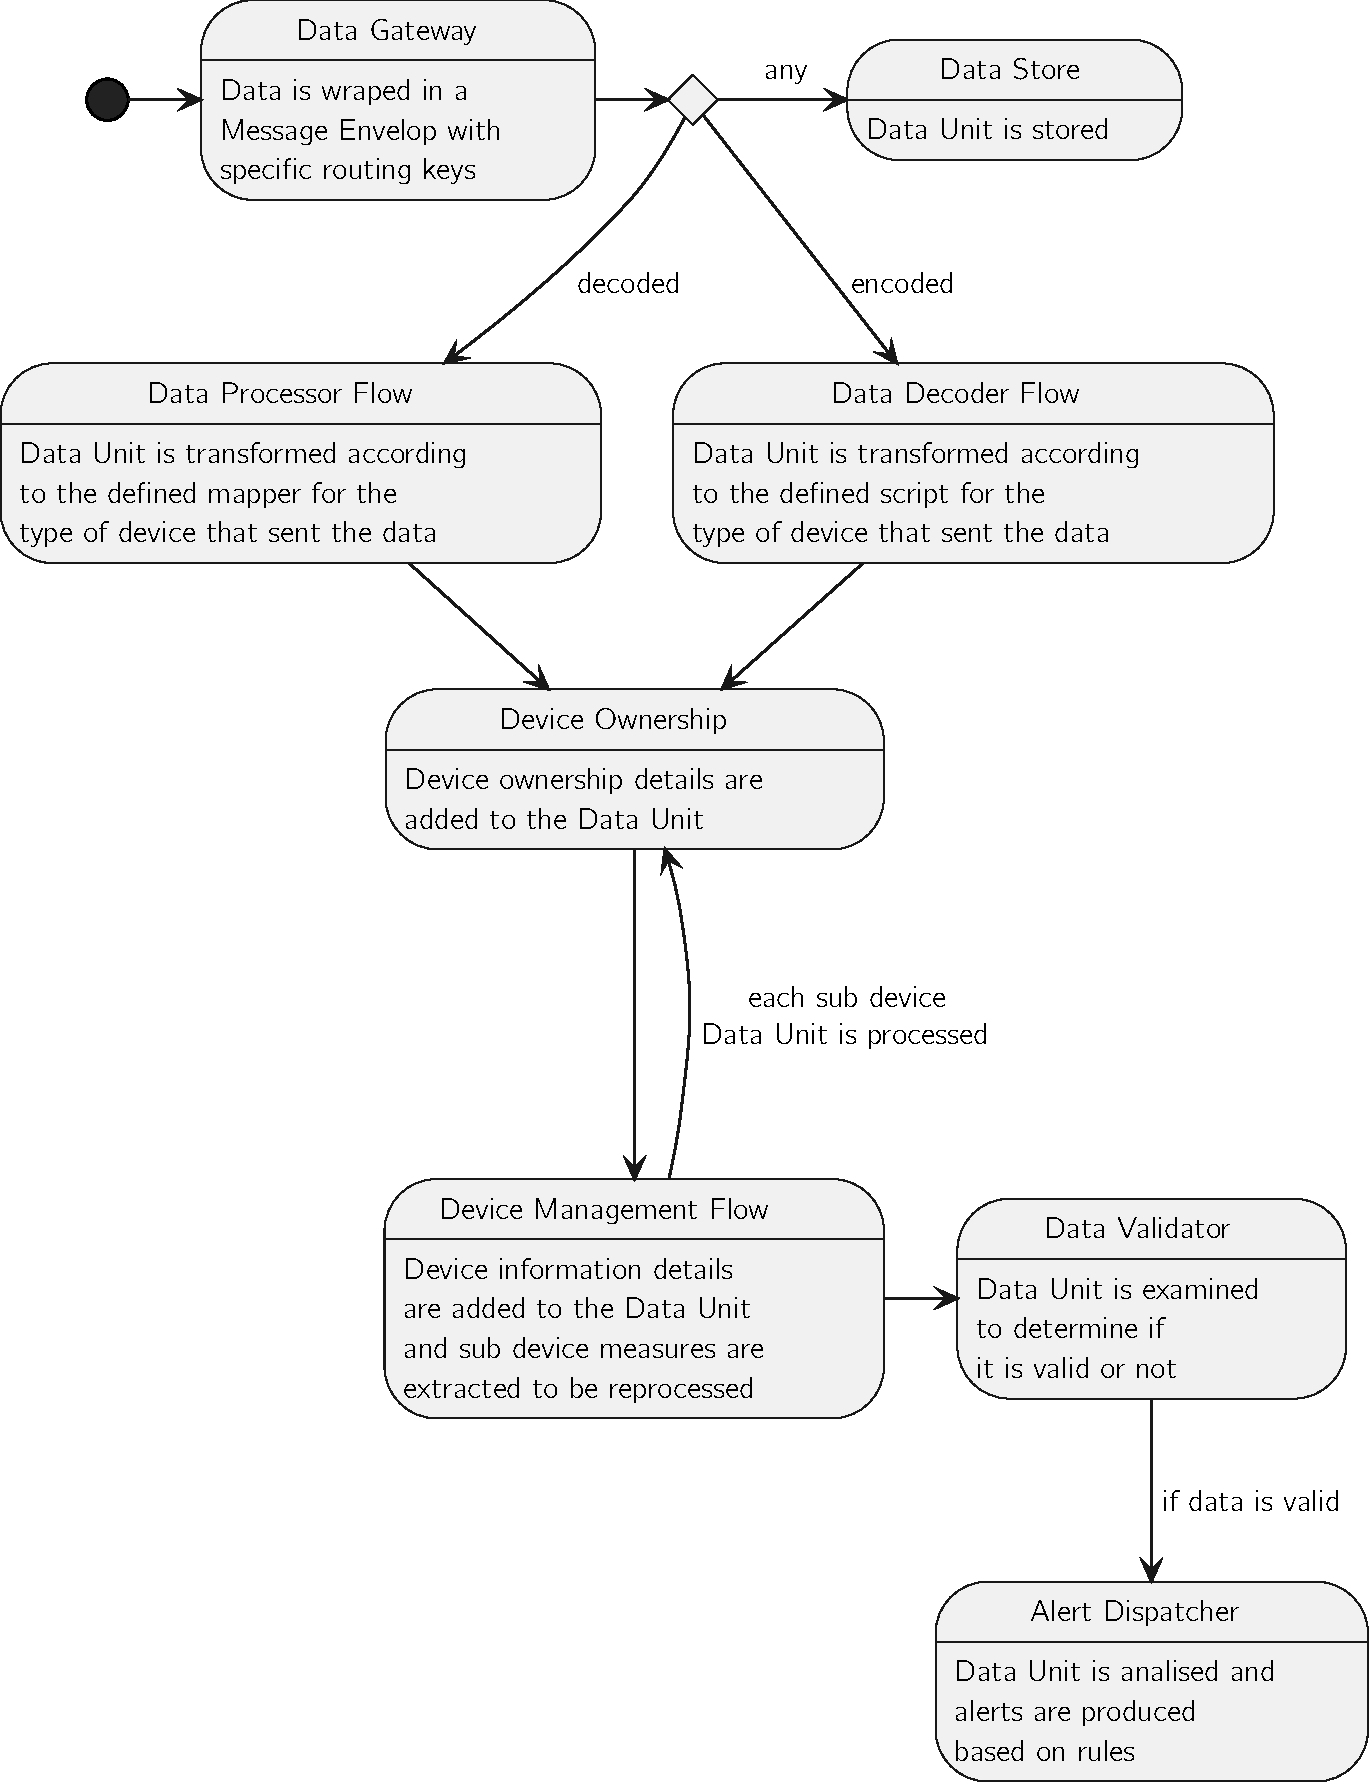
\includegraphics[page=1,width=0.8\columnwidth]{assets/diagrams/design/architectural/level2/process/data-flow-scope.pdf}
   \caption[Data Flow - Container Level - Diagram]{Data Flow - Container Level - Diagram}
   \label{fig:design:architecture:platform:container:process:diagram:flow}
\end{figure}

Most of the containers represented in Figure~\ref{fig:design:architecture:platform:container:process:diagram:flow} have just a portion of their concern's state and may be unable to preform the needed operation on some Data Units. The following diagrams, Figure~\ref{fig:design:architecture:platform:container:process:diagram:decoder:1} and Figure~\ref{fig:design:architecture:platform:container:process:diagram:decoder:2}, addresses how state is managed in Data Decoder Flow Backend and most \textbf{Data Flow Scope} containers.

\begin{figure}
   \centering
   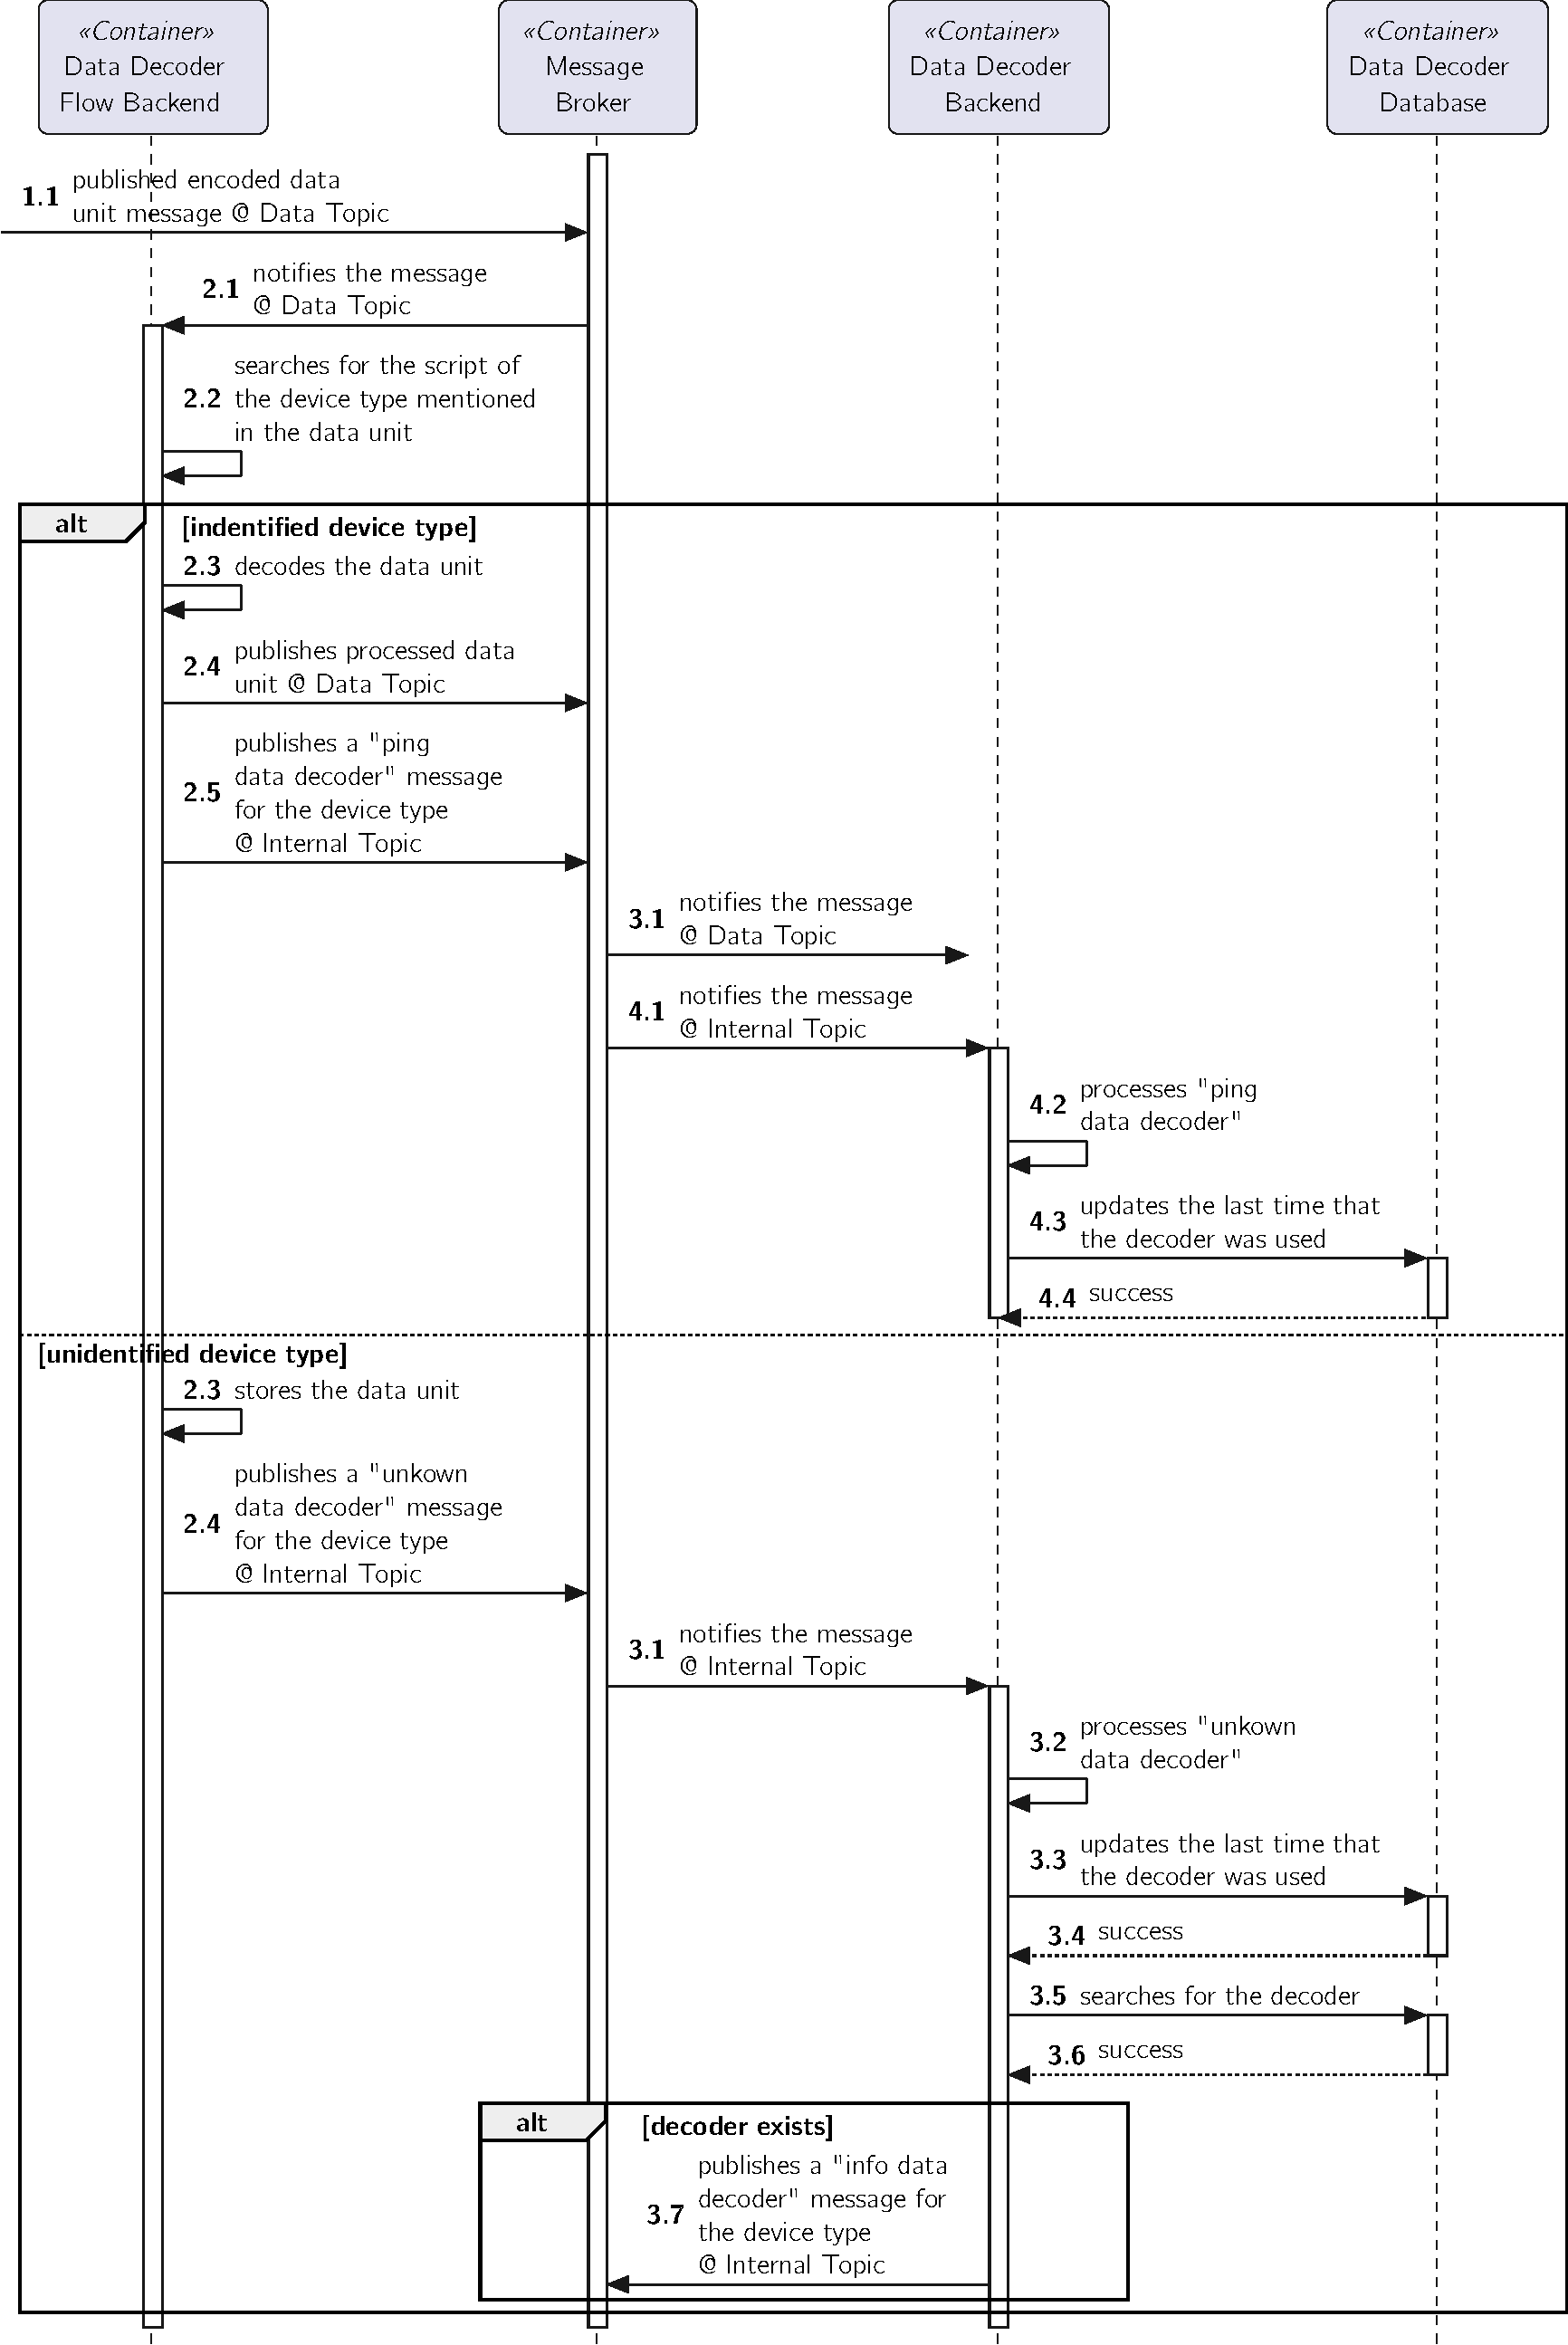
\includegraphics[page=1,width=0.8\columnwidth]{assets/diagrams/design/architectural/level2/process/data-decoder-flow-1.pdf}
   \caption[Data Decoder Operation - Part 1 - Container Level - Process View Diagram]{Data Decoder Operation - Part 1 - Container Level - Process View Diagram}
   \label{fig:design:architecture:platform:container:process:diagram:decoder:1}
\end{figure}

As we can see, in Figure~\ref{fig:design:architecture:platform:container:process:diagram:decoder:1}, the Data Decoder Flow Backend, upon receiving a Data Unit, can preform two operations, depending on whether or not the script is available: decode the Data Unit and notify that the script was used or store the Data Unit and notify that a script for an unknown device type is needed.

The diagram in Figure~\ref{fig:design:architecture:platform:container:process:diagram:decoder:2} describes what happens when a message with a decoder is published (using the \textit{OperationType} Info mentioned in Section~\ref{subsubsec:design:domain:shared_model:routing}).

\begin{figure}[H]
   \centering
   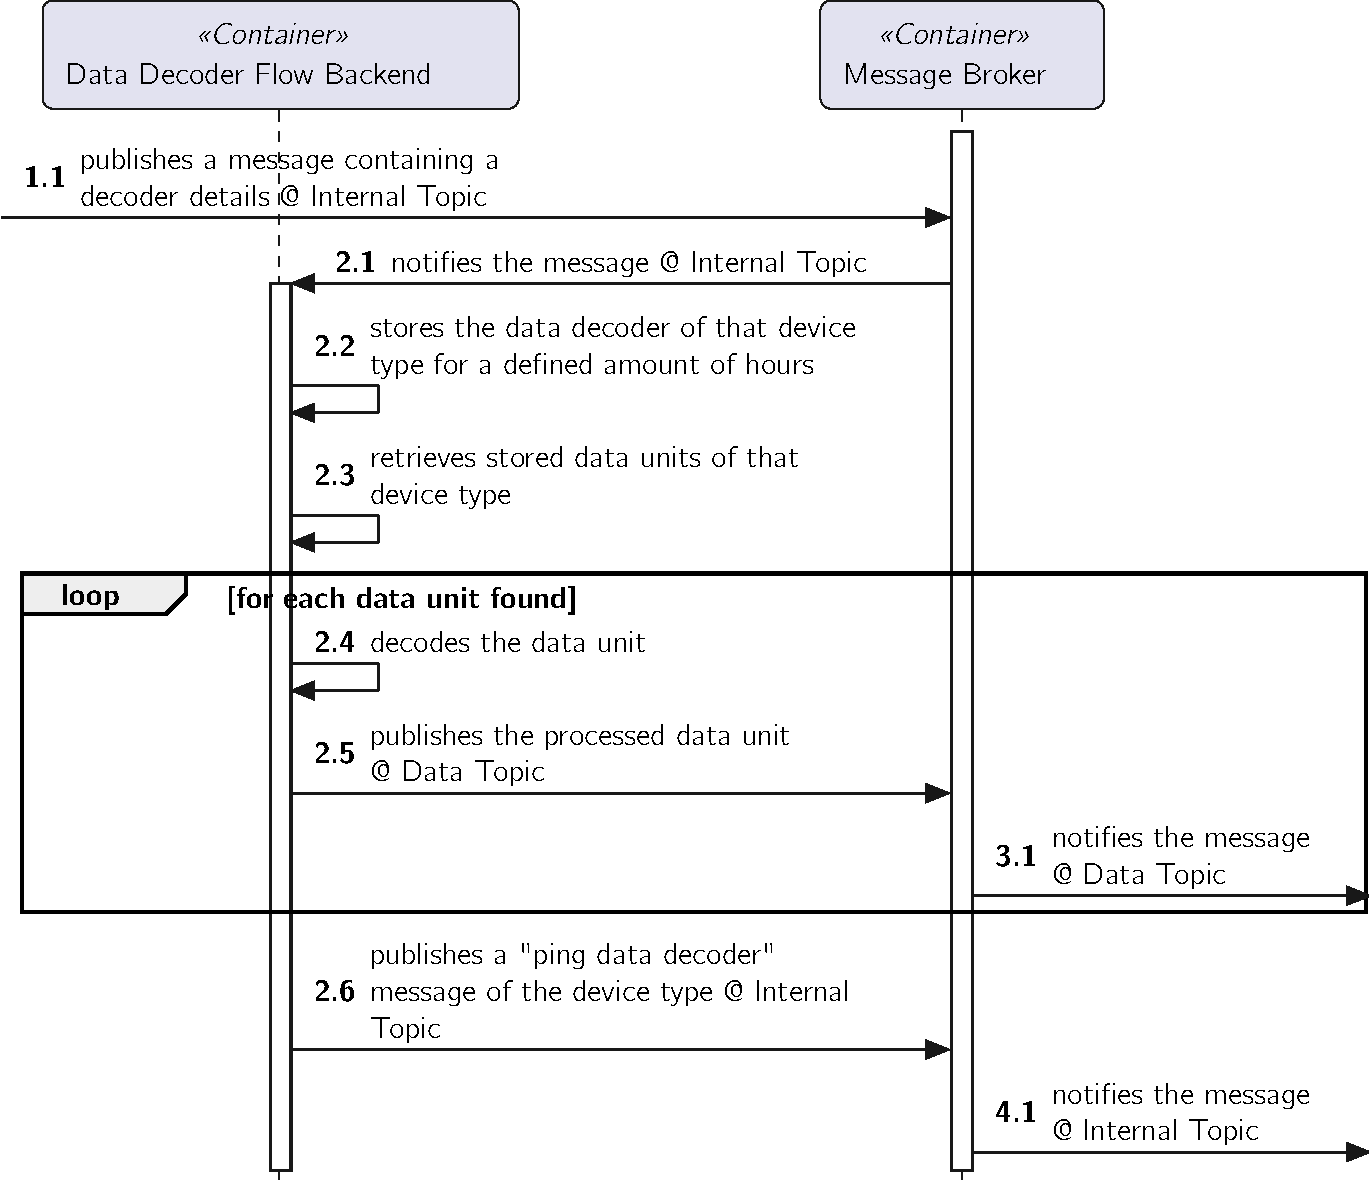
\includegraphics[page=1,width=0.8\columnwidth]{assets/diagrams/design/architectural/level2/process/data-decoder-flow-2.pdf}
   \caption[Data Decoder Operation - Part 2 - Container Level - Process View Diagram]{Data Decoder Operation - Part 2 - Container Level - Process View Diagram}
   \label{fig:design:architecture:platform:container:process:diagram:decoder:2}
\end{figure}

As we can see, in Figure~\ref{fig:design:architecture:platform:container:process:diagram:decoder:2}, Data Decoder Flow Backend, upon receiving an info regarding a data decoder, searches for unhandled Data Units and processes them.
To minimize the memory in use, a data decoder has to be continually used in order for it to remain in cache. As seen in step \textbf{2.2}, if \textit{X} hours pass since the last time a decoder was used it is evicted from the container internal state.

The operations described here for the Data Decoder Flow Backend are replicated in the following concerns/containers:

\begin{itemize}
   \item \textbf{Data Processor Context}: Data Processor Flow Backend;
   \item \textbf{Device Management Context}: Device Management Flow Backend and Device Commander Backend;
   \item \textbf{Identity Management Context}: Device Ownership.
\end{itemize}

As described before, containers that belong to the \textbf{Data Flow Scope} operate according to what the \textbf{Configuration Scope} defined.

The next diagrams, in Figure~\ref{fig:design:architecture:platform:container:process:diagram:processor} and Figure~\ref{fig:design:architecture:platform:container:process:diagram:device} present some of the common operations that happen in that scope.

\begin{figure}
   \centering
   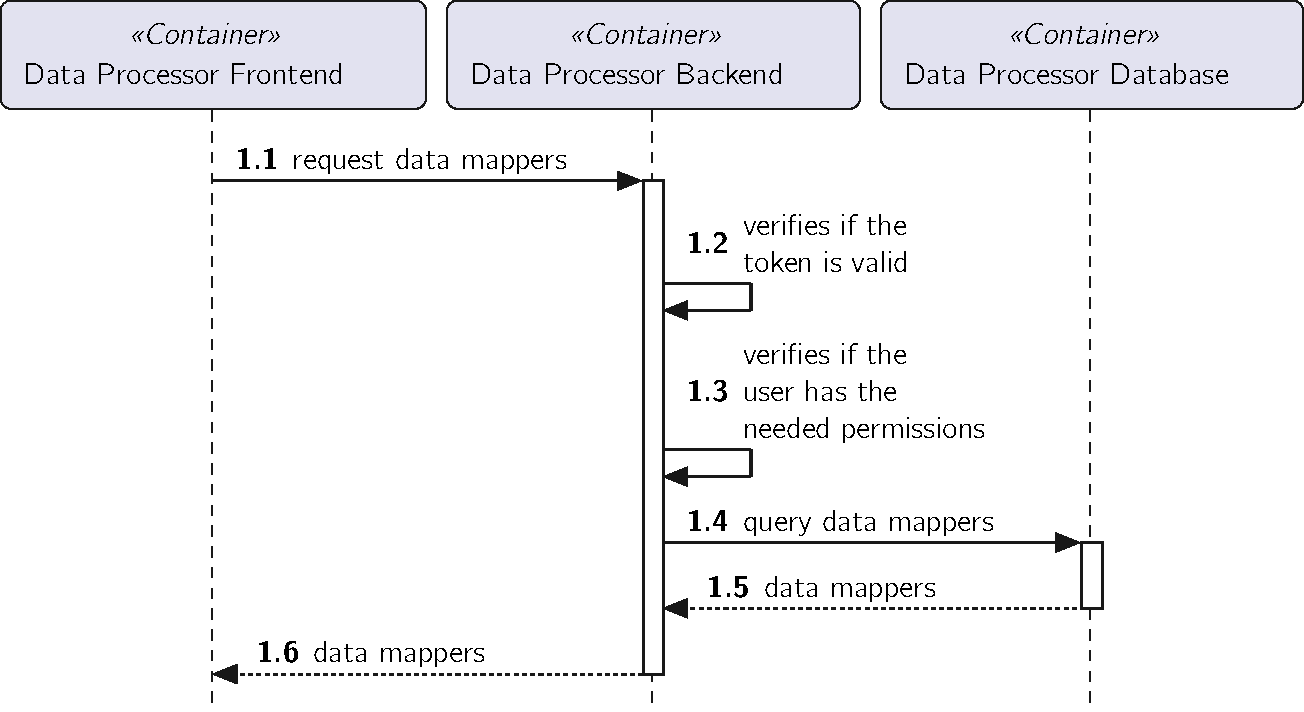
\includegraphics[page=1,width=0.8\columnwidth]{assets/diagrams/design/architectural/level2/process/consult-data-processor.pdf}
   \caption[Consult Data Processors - Container Level - Process View Diagram]{Consult Data Processors - Container Level - Process View Diagram}
   \label{fig:design:architecture:platform:container:process:diagram:processor}
\end{figure}

The diagram presented in Figure~\ref{fig:design:architecture:platform:container:process:diagram:processor} represents a simple consult of data mappers, as we can see, only the Data Processor Context in the Configuration Scope is invoked. When a change to the state is made in any Context of the Configuration Scope, events are published. The next diagram, Figure~\ref{fig:design:architecture:platform:container:process:diagram:device} displays an example of this occurrence.

\begin{figure}
   \centering
   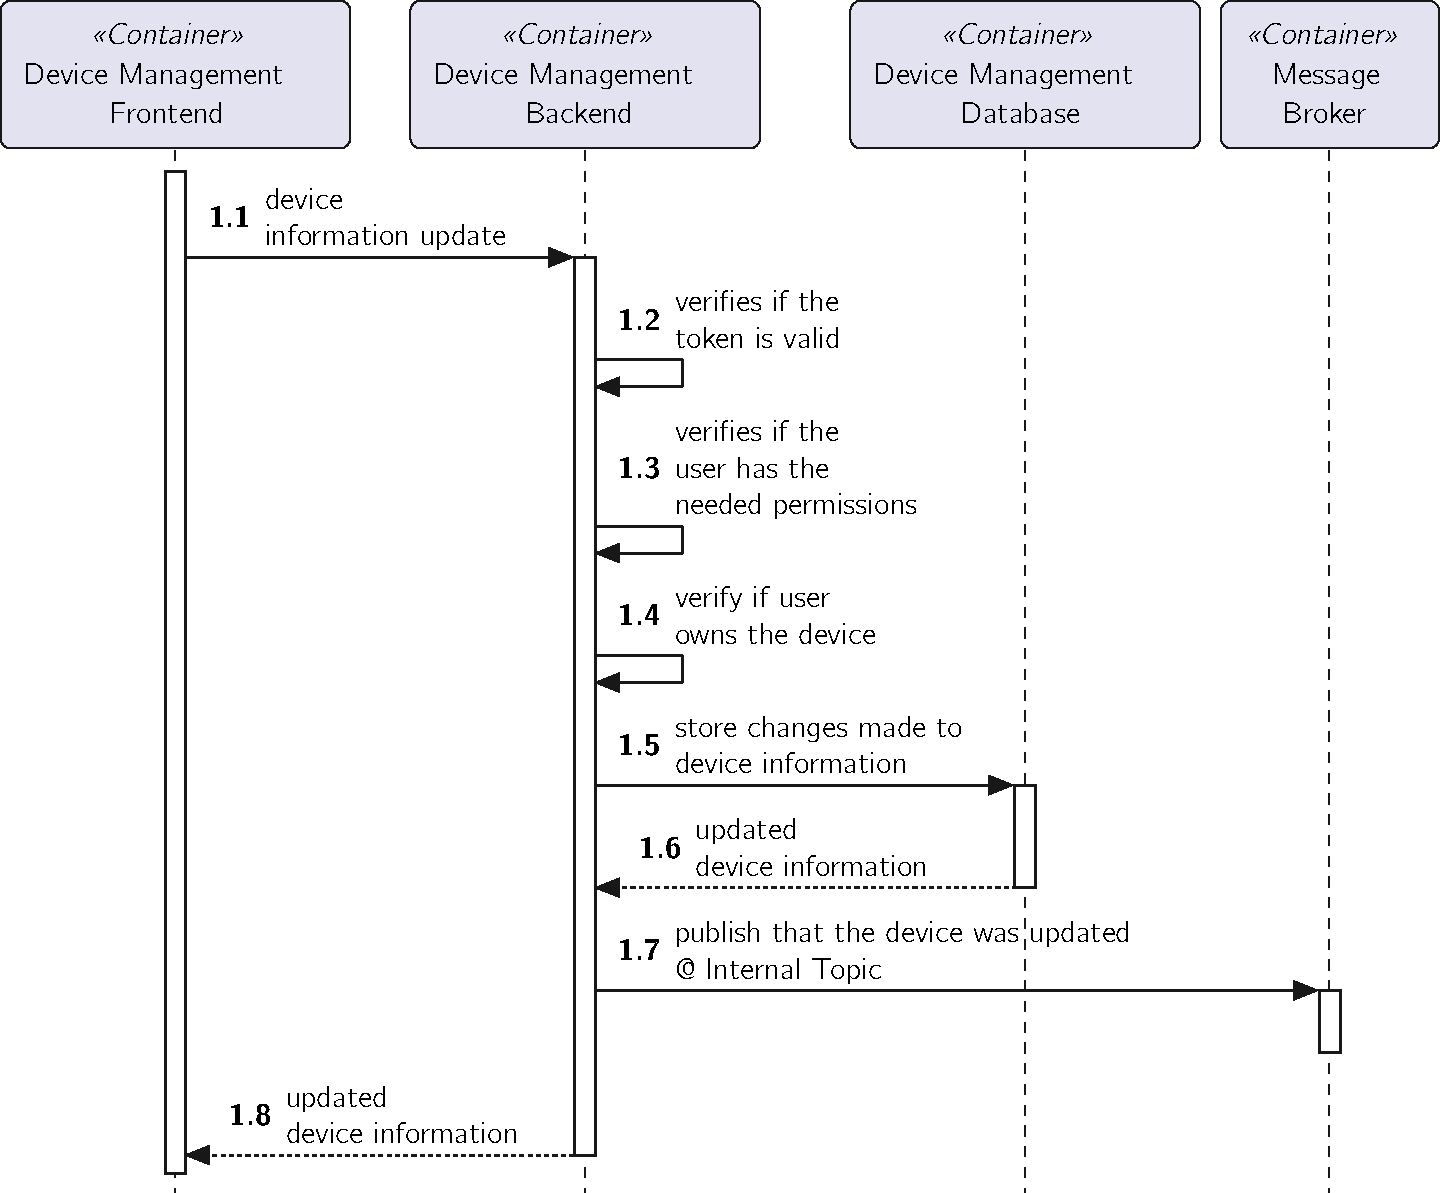
\includegraphics[page=1,width=0.8\columnwidth]{assets/diagrams/design/architectural/level2/process/edit-device-management.pdf}
   \caption[Edit Device Information - Container Level - Process View Diagram]{Edit Device Information - Container Level - Process View Diagram}
   \label{fig:design:architecture:platform:container:process:diagram:device}
\end{figure}

In this use case - Figure~\ref{fig:design:architecture:platform:container:process:diagram:device} - a device information is changed. Since this operation changes the internal state of the device management concern, an event is published in the Internal Topic.

According to the Section~\ref{subsubsec:design:domain:shared_model:routing}, this specific event uses the following \textit{Routing Keys}:

\begin{itemize}
   \item \textbf{Protocol Version}: the version of \textit{iot-core} currently in use by Device Management Backend;
   \item \textbf{Container Type}: Device Management Backend;
   \item \textbf{Topic Type}: Internal;
   \item \textbf{Operation Type}: Info;
   \item \textbf{Context Type}: Device Management.
\end{itemize}

There are three containers that subscribe to this specific type of event:

\begin{itemize}
   \item \textbf{Device Management Flow Backend}: so that the Data Units of the device changed are enriched with the latest information;
   \item \textbf{Device Command Backend}: so that commands for this device are treated according to the latest information;
   \item \textbf{Identity Management Backend}: so that information related to the device changed is presented according to the latest update. This container maintains local copies of all devices names to present to the user without needing to request Device Management for that information every time.
\end{itemize}

The step \textbf{1.3} in the last two diagrams (Figure~\ref{fig:design:architecture:platform:container:process:diagram:processor} and \ref{fig:design:architecture:platform:container:process:diagram:device}) references user permissions but there is no mention of how this permissions are associated to the user. In the next diagrams - Figure~\ref{fig:design:architecture:platform:container:process:diagram:authentication} and Figure~\ref{fig:design:architecture:platform:container:process:diagram:authorization} - authentication and authorization in the \textbf{Sensae Console} are addressed, other approaches are discussed in Appendix~\ref{appendix:design:alternatives:auth}.

The system verifies the identity of a user based on the authentication performed by an external \gls{CIAM} solution using OpenID Connect 1.0, \cite{openid}, an identity layer on top of the OAuth 2.0 protocol. According to \cite{oauth} OAuth2.0 ``enables a third-party application to obtain limited access to an HTTP service''. In this situation the Frontend of \textbf{Sensae Console} is the third-party application and the HTTP service is any of the \textbf{Sensae Console} backend services.

\begin{figure}
   \centering
   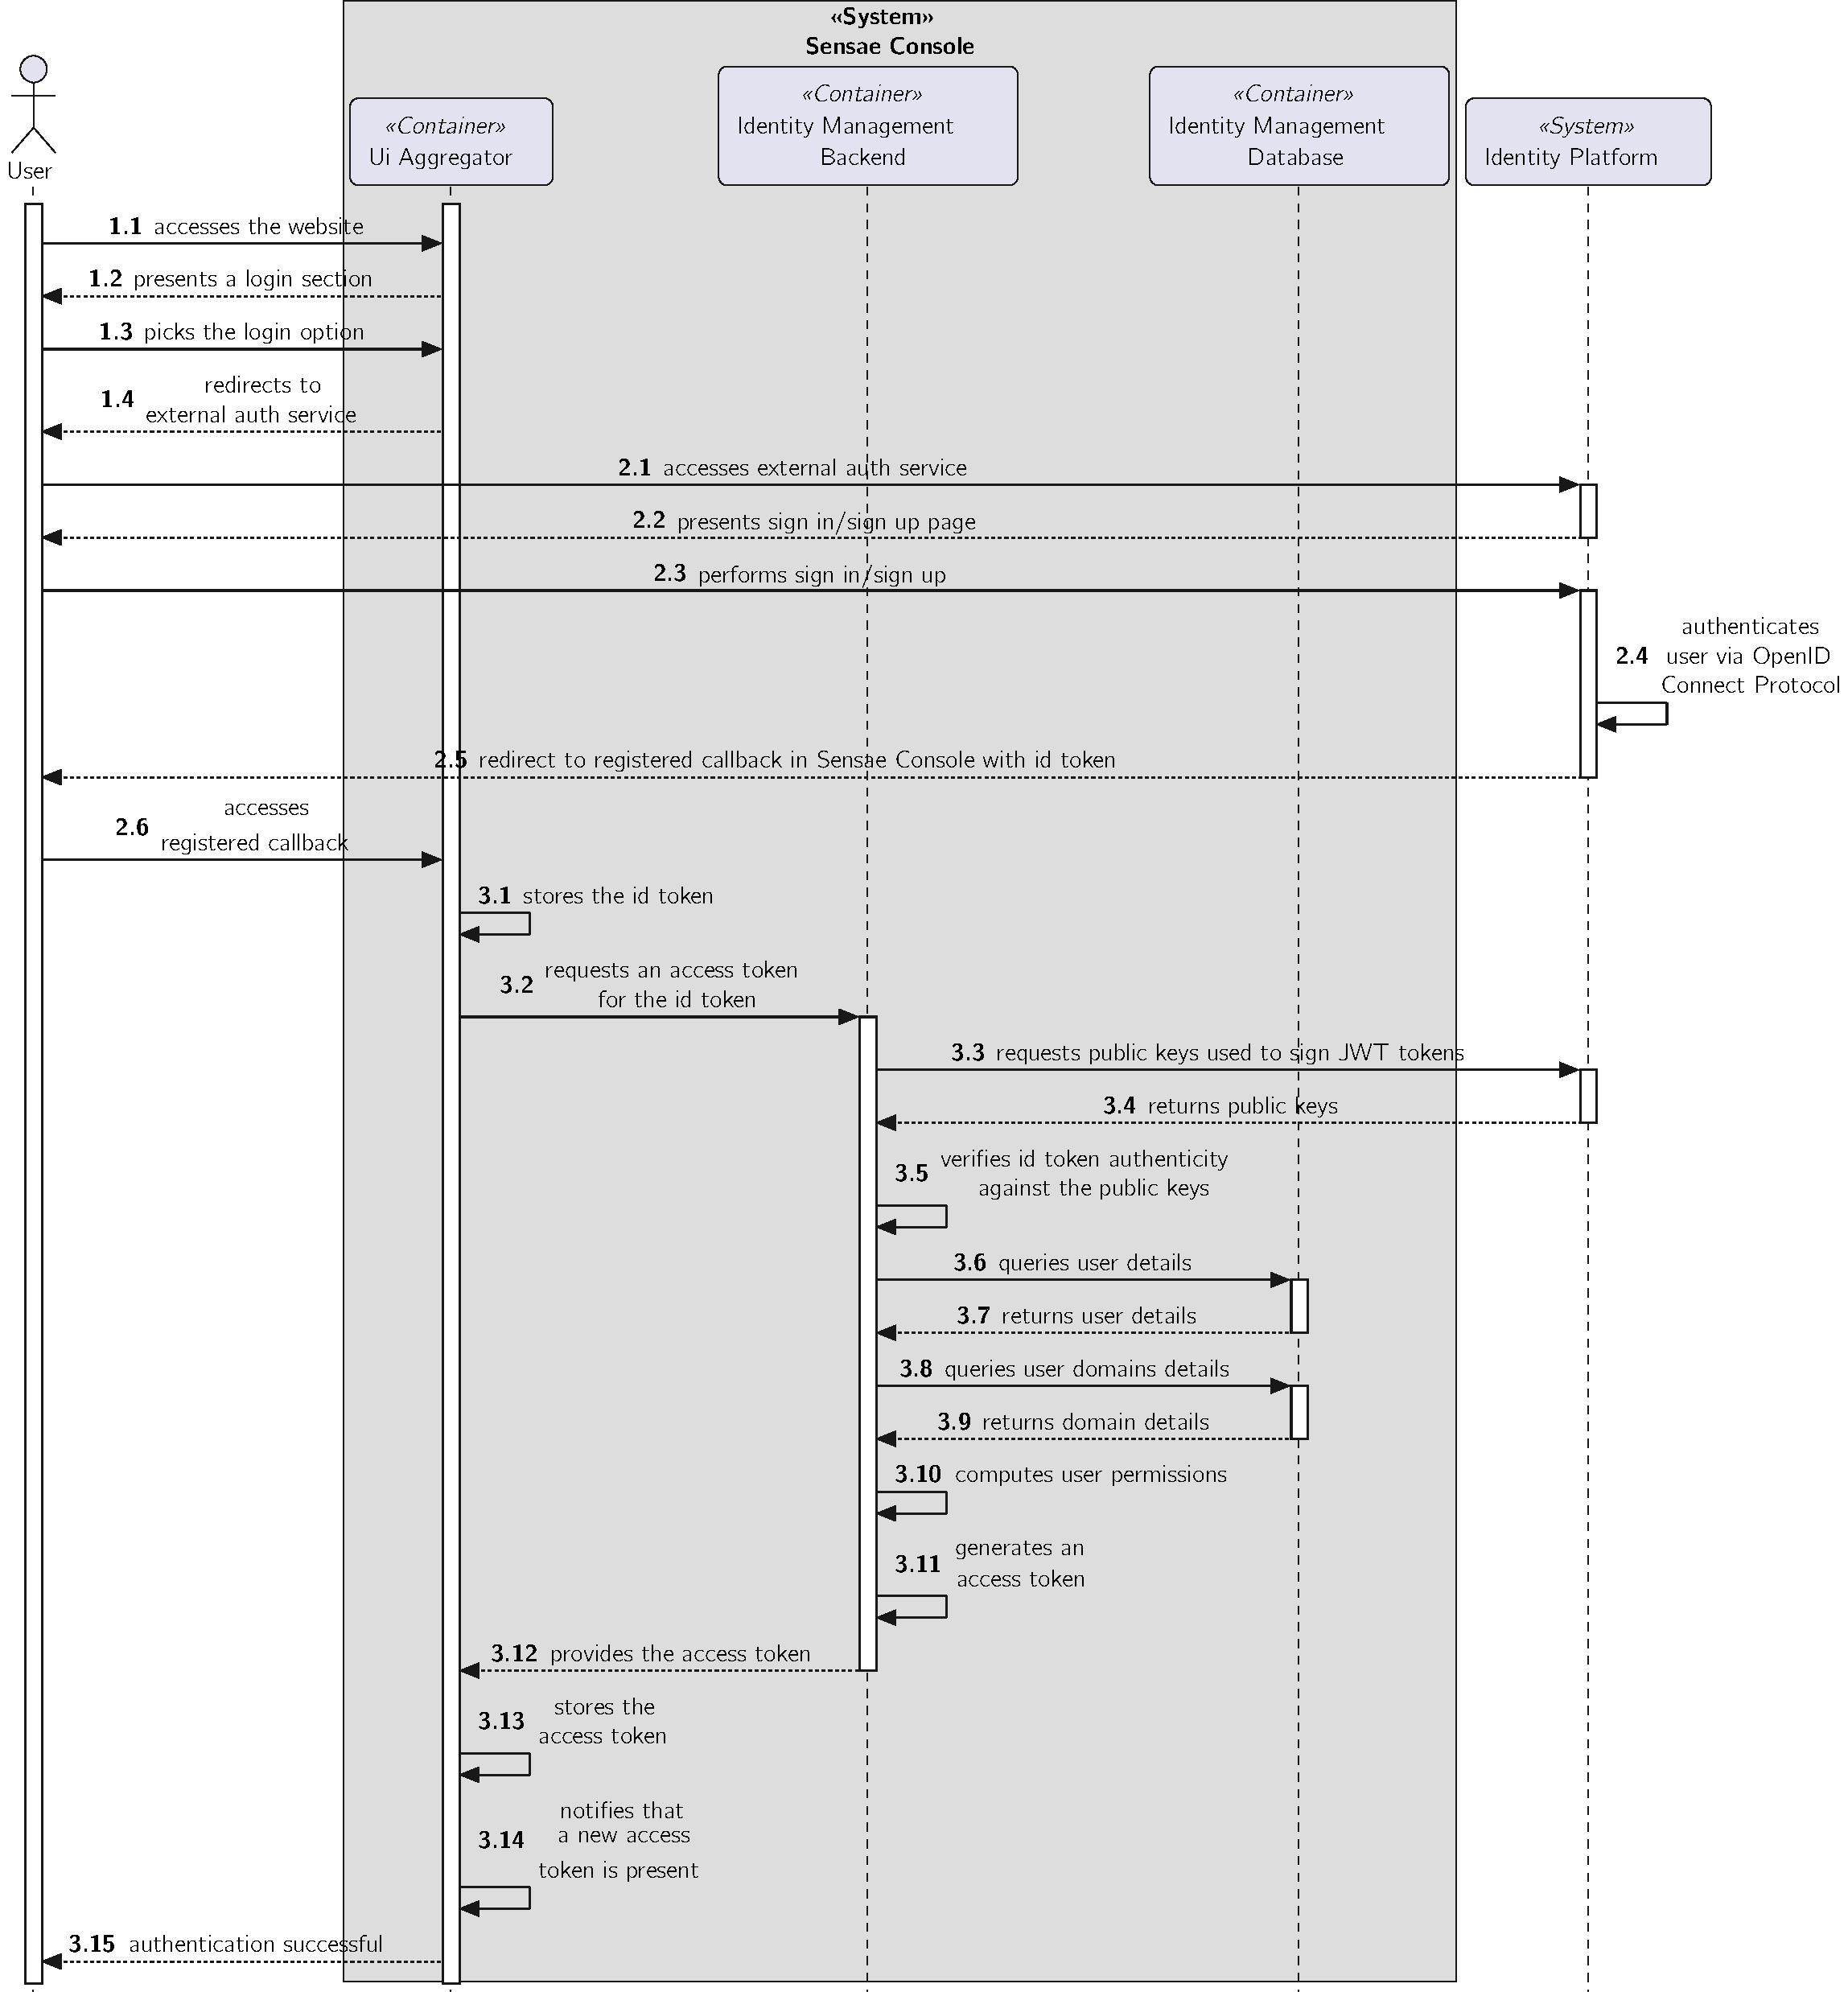
\includegraphics[page=1,width=\columnwidth]{assets/diagrams/design/architectural/level2/process/user-authentication.pdf}
   \caption[User Authentication - Container Level - Process View Diagram]{User Authentication - Container Level - Process View Diagram}
   \label{fig:design:architecture:platform:container:process:diagram:authentication}
\end{figure}

The diagram in Figure~\ref{fig:design:architecture:platform:container:process:diagram:authentication} illustrates how a user can authenticate against \textbf{Sensae Console}.
The user identity and credentials validation are assured by an external identity platform such as \citetitle{googleid} or \citetitle{azureid}. Once an \textit{id token} is provided to \textbf{Sensae Console} it can use it to verify the user identity against the local registry. To ensure that the \textit{id token} is valid, Identity Management Backend checks if it was signed by the platform that supposedly issued it (step \textbf{3.3} and \textbf{3.5}). After validating the \textit{id token} it searches for the needed information to create an \textit{access token} and then provides it. The \textit{access token} can then be used for a limited time to access any protected HTTP resource of \textbf{Sensae Console} as demonstrated in Figure~\ref{fig:design:architecture:platform:container:process:diagram:authorization}.

\begin{figure}[H]
   \centering
   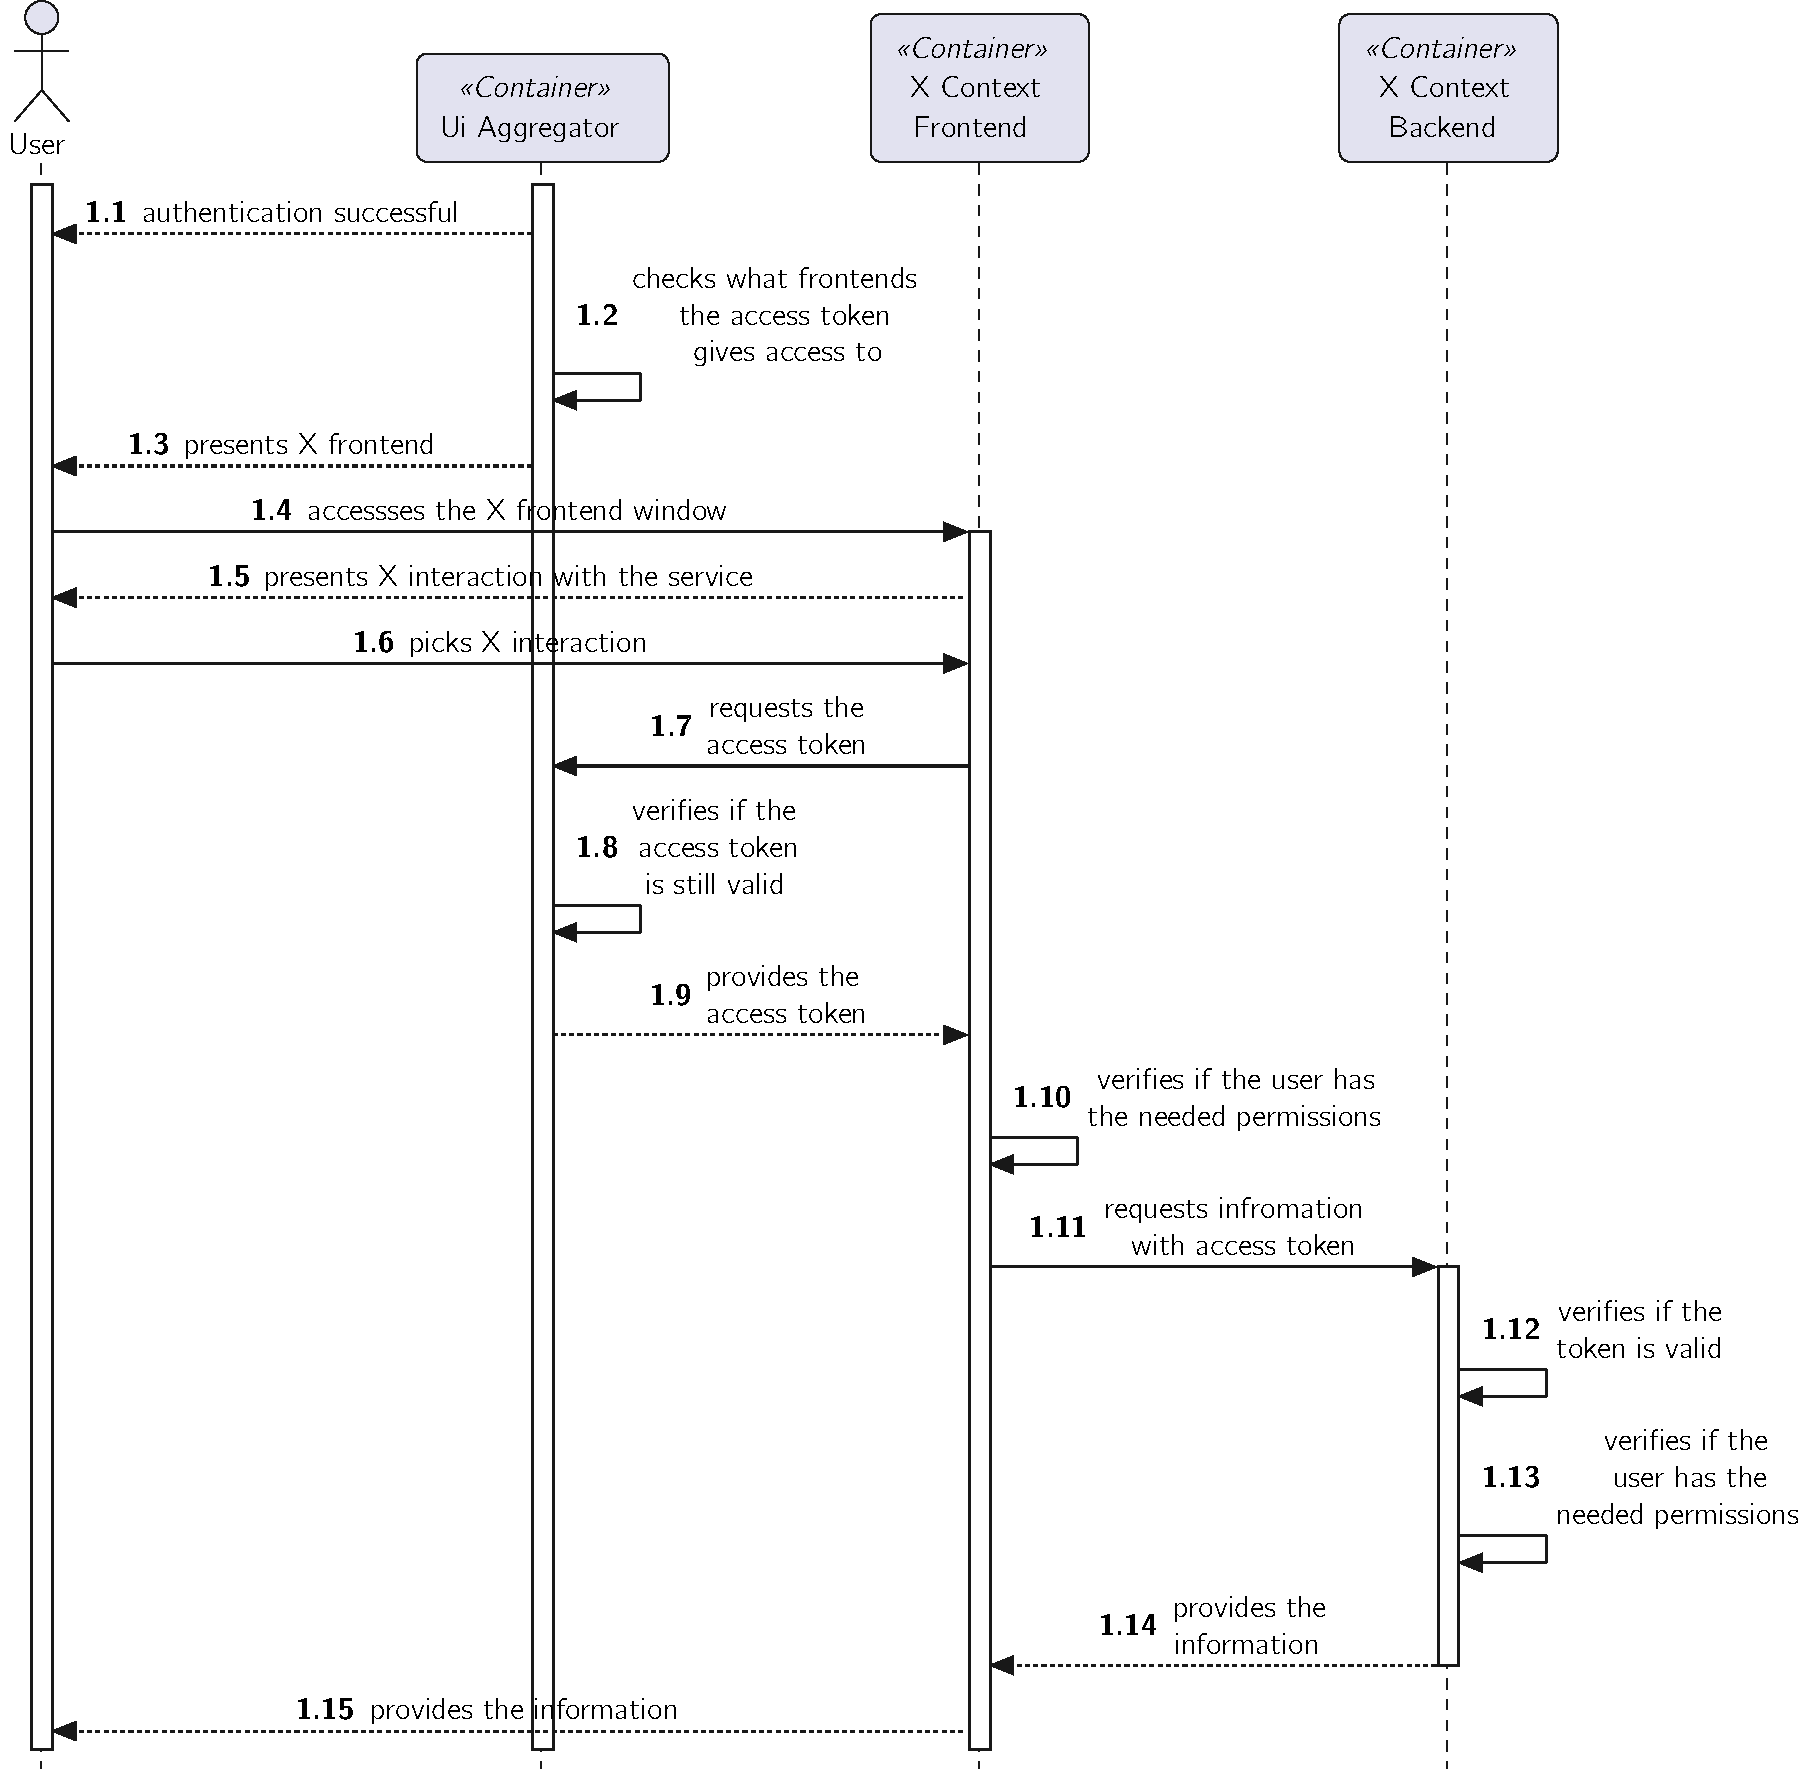
\includegraphics[page=1,width=0.8\columnwidth]{assets/diagrams/design/architectural/level2/process/user-authorization.pdf}
   \caption[User Authorization - Container Level - Process View Diagram]{User Authorization - Container Level - Process View Diagram}
   \label{fig:design:architecture:platform:container:process:diagram:authorization}
\end{figure}

In this diagram, Figure~\ref{fig:design:architecture:platform:container:process:diagram:authorization}, the expected behavior for any pair of frontend and backend containers in \textbf{Configuration Scope} (and \textbf{Business Applications}, when served from the \textbf{UI Aggregator}) is presented. Each frontend displays only the actions and information that the user permissions allow. The user permissions are once again verified in the backend to secure the system against malicious accesses. Other alternatives related to authentication and authorization are presented in  Appendix~\ref{appendix:design:alternatives:auth}.

\subsubsection{Container Level - Implementation View}
\label{par:design:architecture:platform:container:development}

Each container mentioned in the Section~\ref{par:design:architecture:platform:container:logical} is developed inside the same package, \textit{sensae-console}. The following diagrams presents how containers are mapped to packages.

The following diagrams are divided into:

\begin{itemize}
   \item Backend Containers: Figure~\ref{fig:design:architecture:platform:container:development:backend};
   \item Database Containers: Figure~\ref{fig:design:architecture:platform:container:development:database};
   \item Frontend Containers: Figure~\ref{fig:design:architecture:platform:container:development:frontend}.
\end{itemize}

Backend services are organized according to the diagram in Figure~\ref{fig:design:architecture:platform:container:development:backend}.

Each backend service container is mapped to its own individual package. The Data Relayer Container was the only one configured, all others were developed.

\begin{figure}[H]
   \centering
   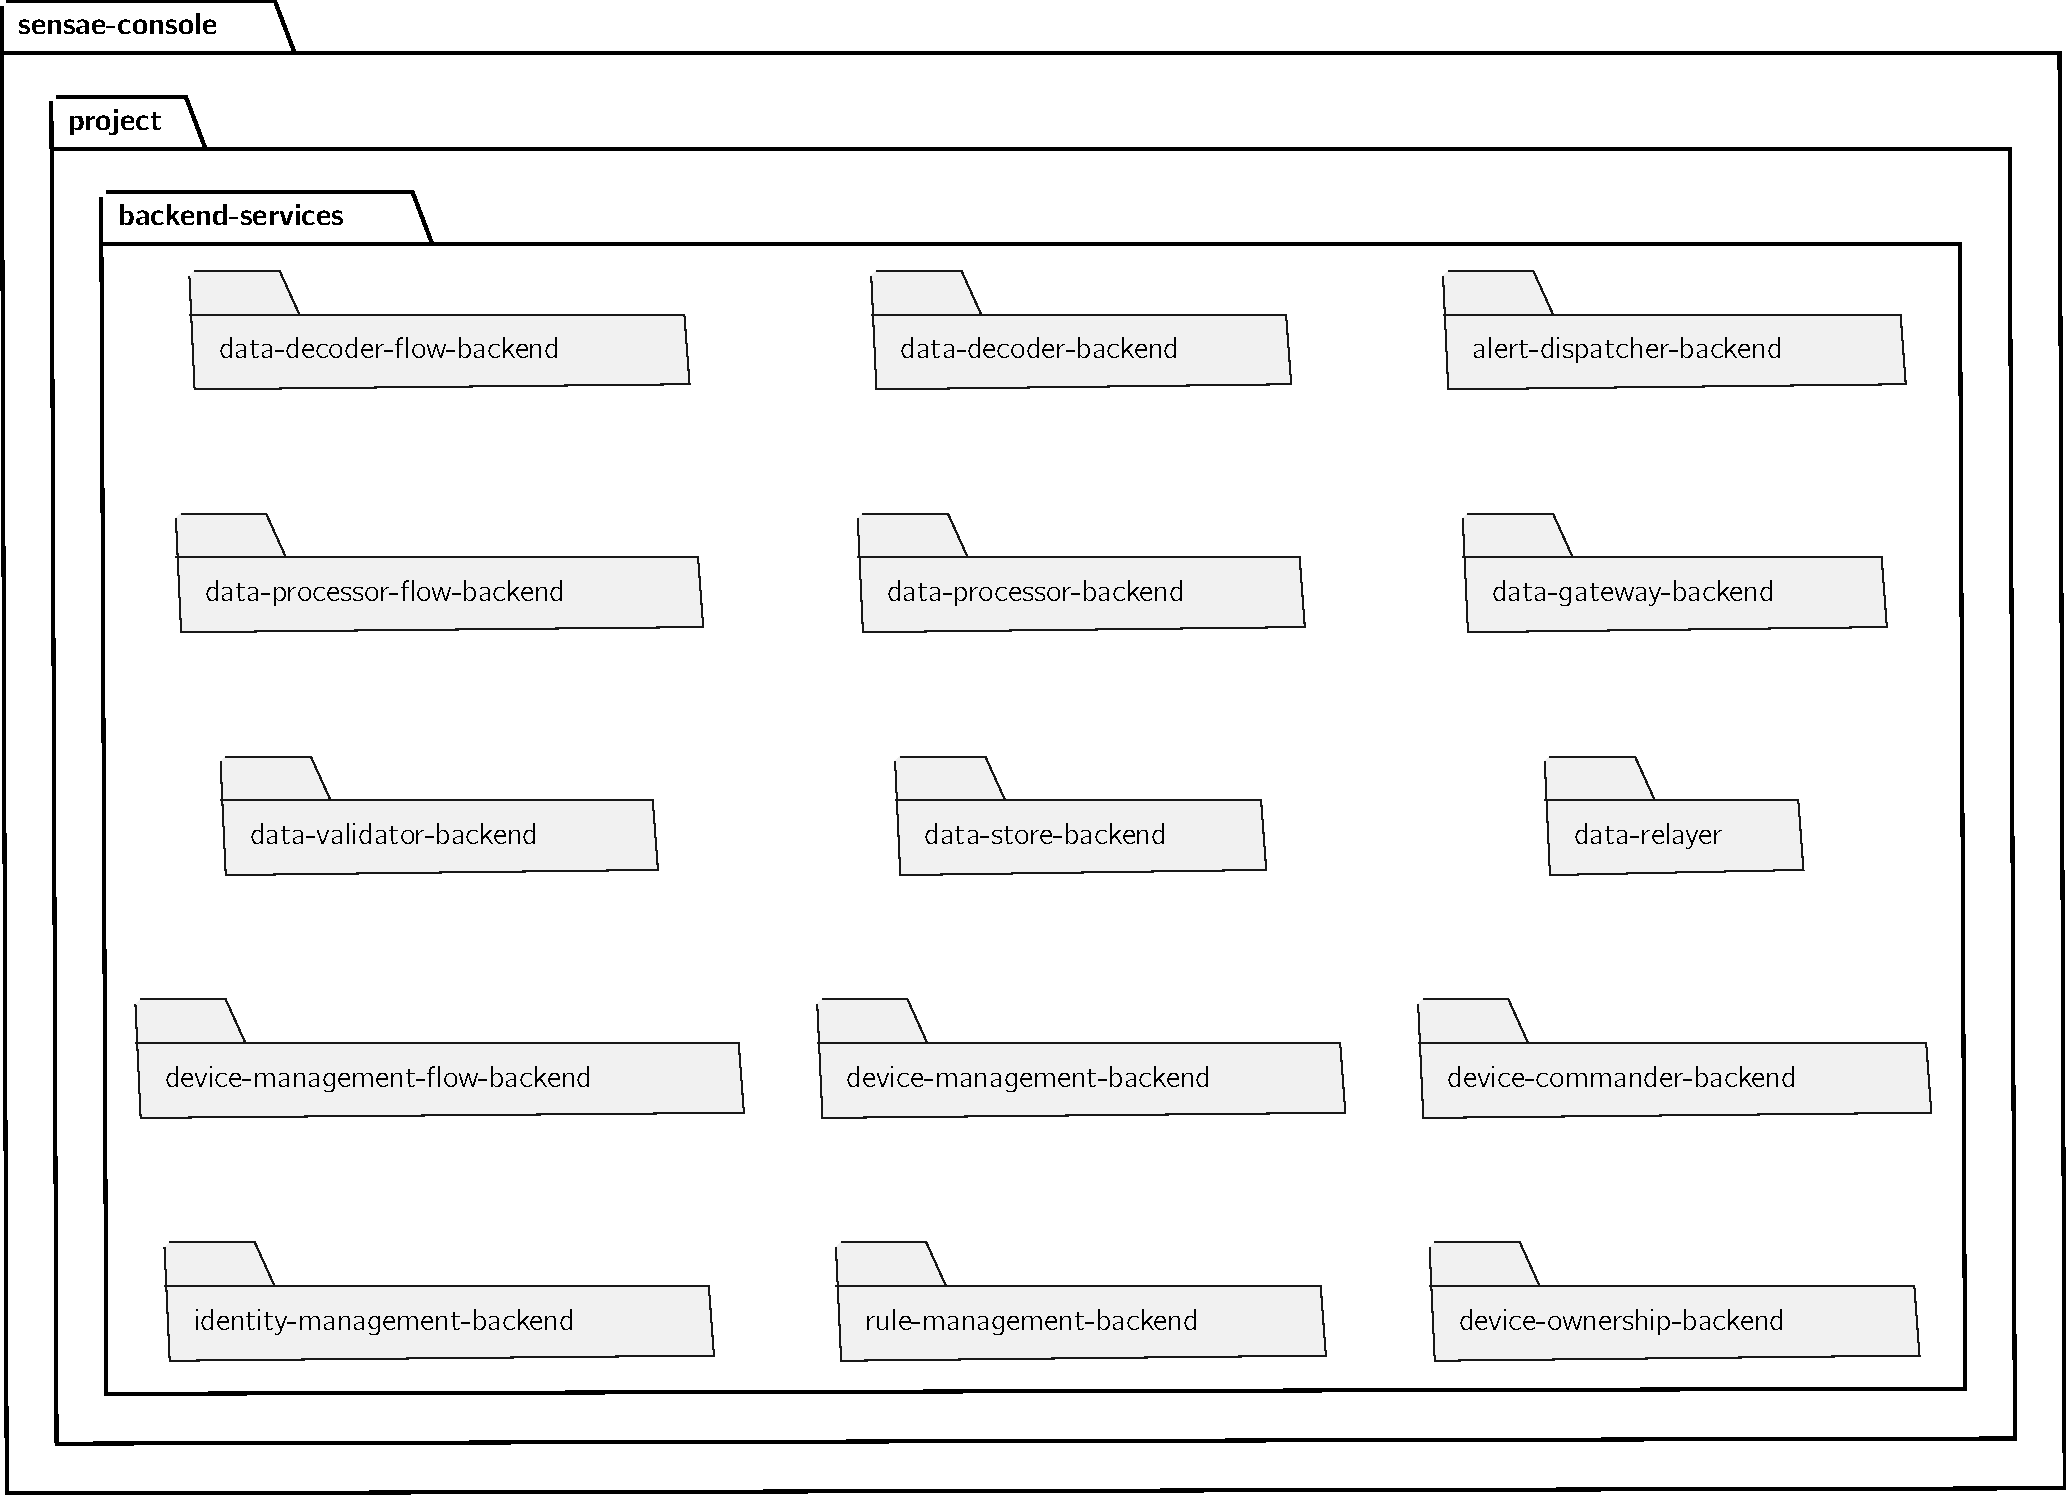
\includegraphics[page=1,width=\columnwidth]{assets/diagrams/design/architectural/level2/development/backend.pdf}
   \caption[Container Level - Implementation View Diagram]{Backend Services - Container Level - Implementation View Diagram}
   \label{fig:design:architecture:platform:container:development:backend}
\end{figure}

Database services are organized according to the diagram in Figure~\ref{fig:design:architecture:platform:container:development:database}.

No database service has been developed, only configured. The Message Broker also has no package in the project since it didn't need any configuration and wasn't developed.

\begin{figure}[H]
   \centering
   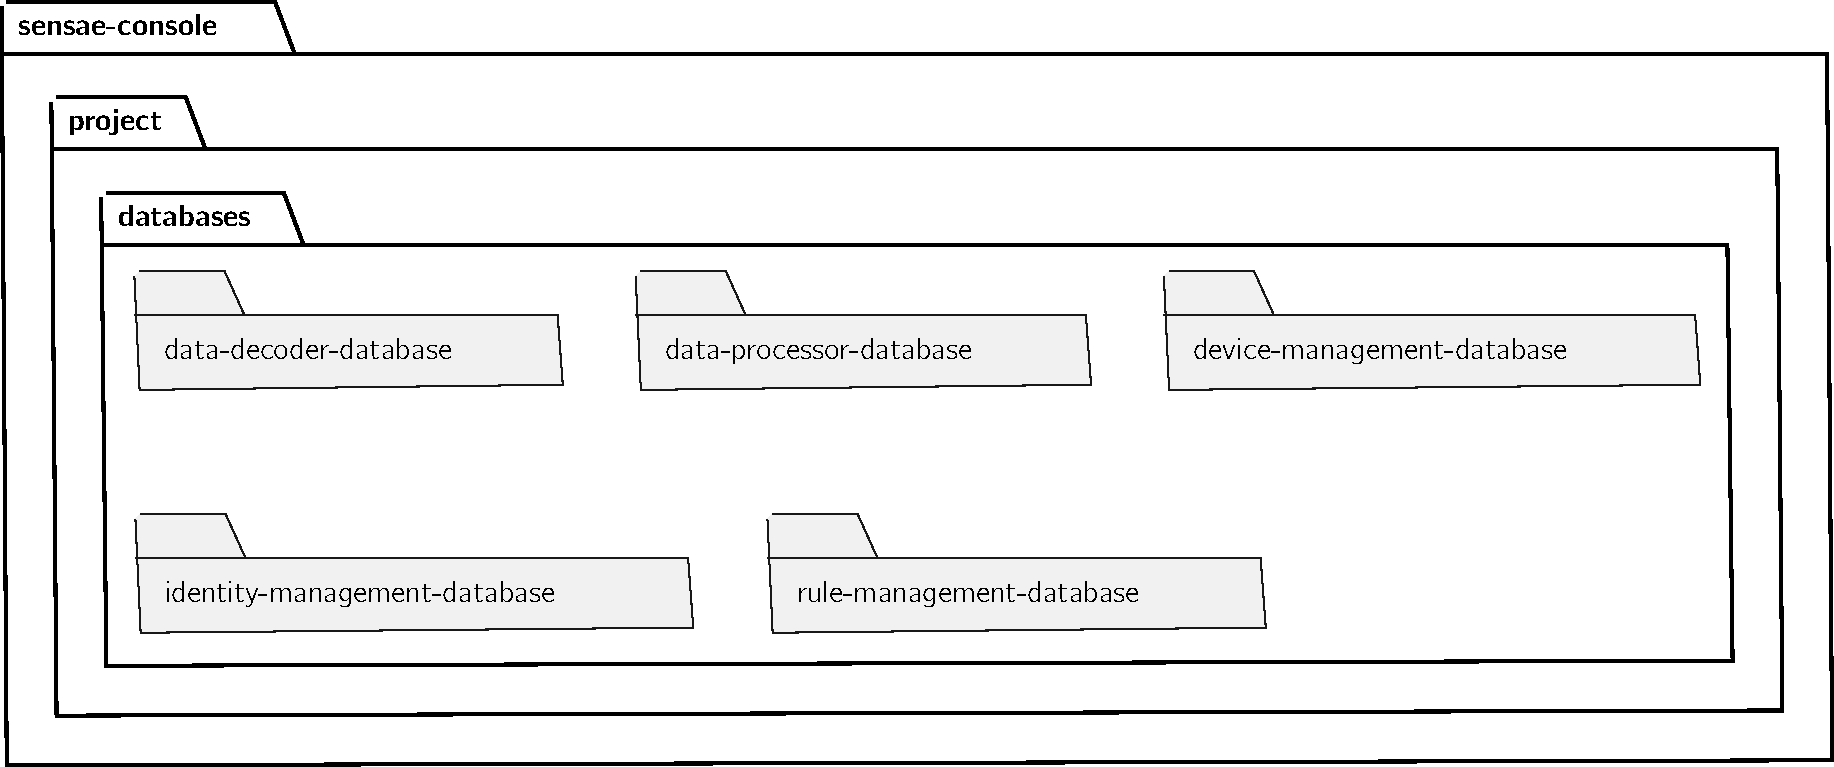
\includegraphics[page=1,width=\columnwidth]{assets/diagrams/design/architectural/level2/development/database.pdf}
   \caption[Database Services - Container Level - Implementation View Diagram]{Database Services - Container Level - Implementation View Diagram}
   \label{fig:design:architecture:platform:container:development:database}
\end{figure}

Frontend services are organized according to the diagram in Figure~\ref{fig:design:architecture:platform:container:development:frontend}.

Each frontend service is divided between the \textit{apps} package and \textit{libs} package. Each \textit{app} depends on the corresponding \textit{lib}. Every \textit{lib} depend on the \textit{core} and \textit{auth} packages. The UI Aggregator depends only on the \textit{auth} package.

\begin{figure}[H]
   \centering
   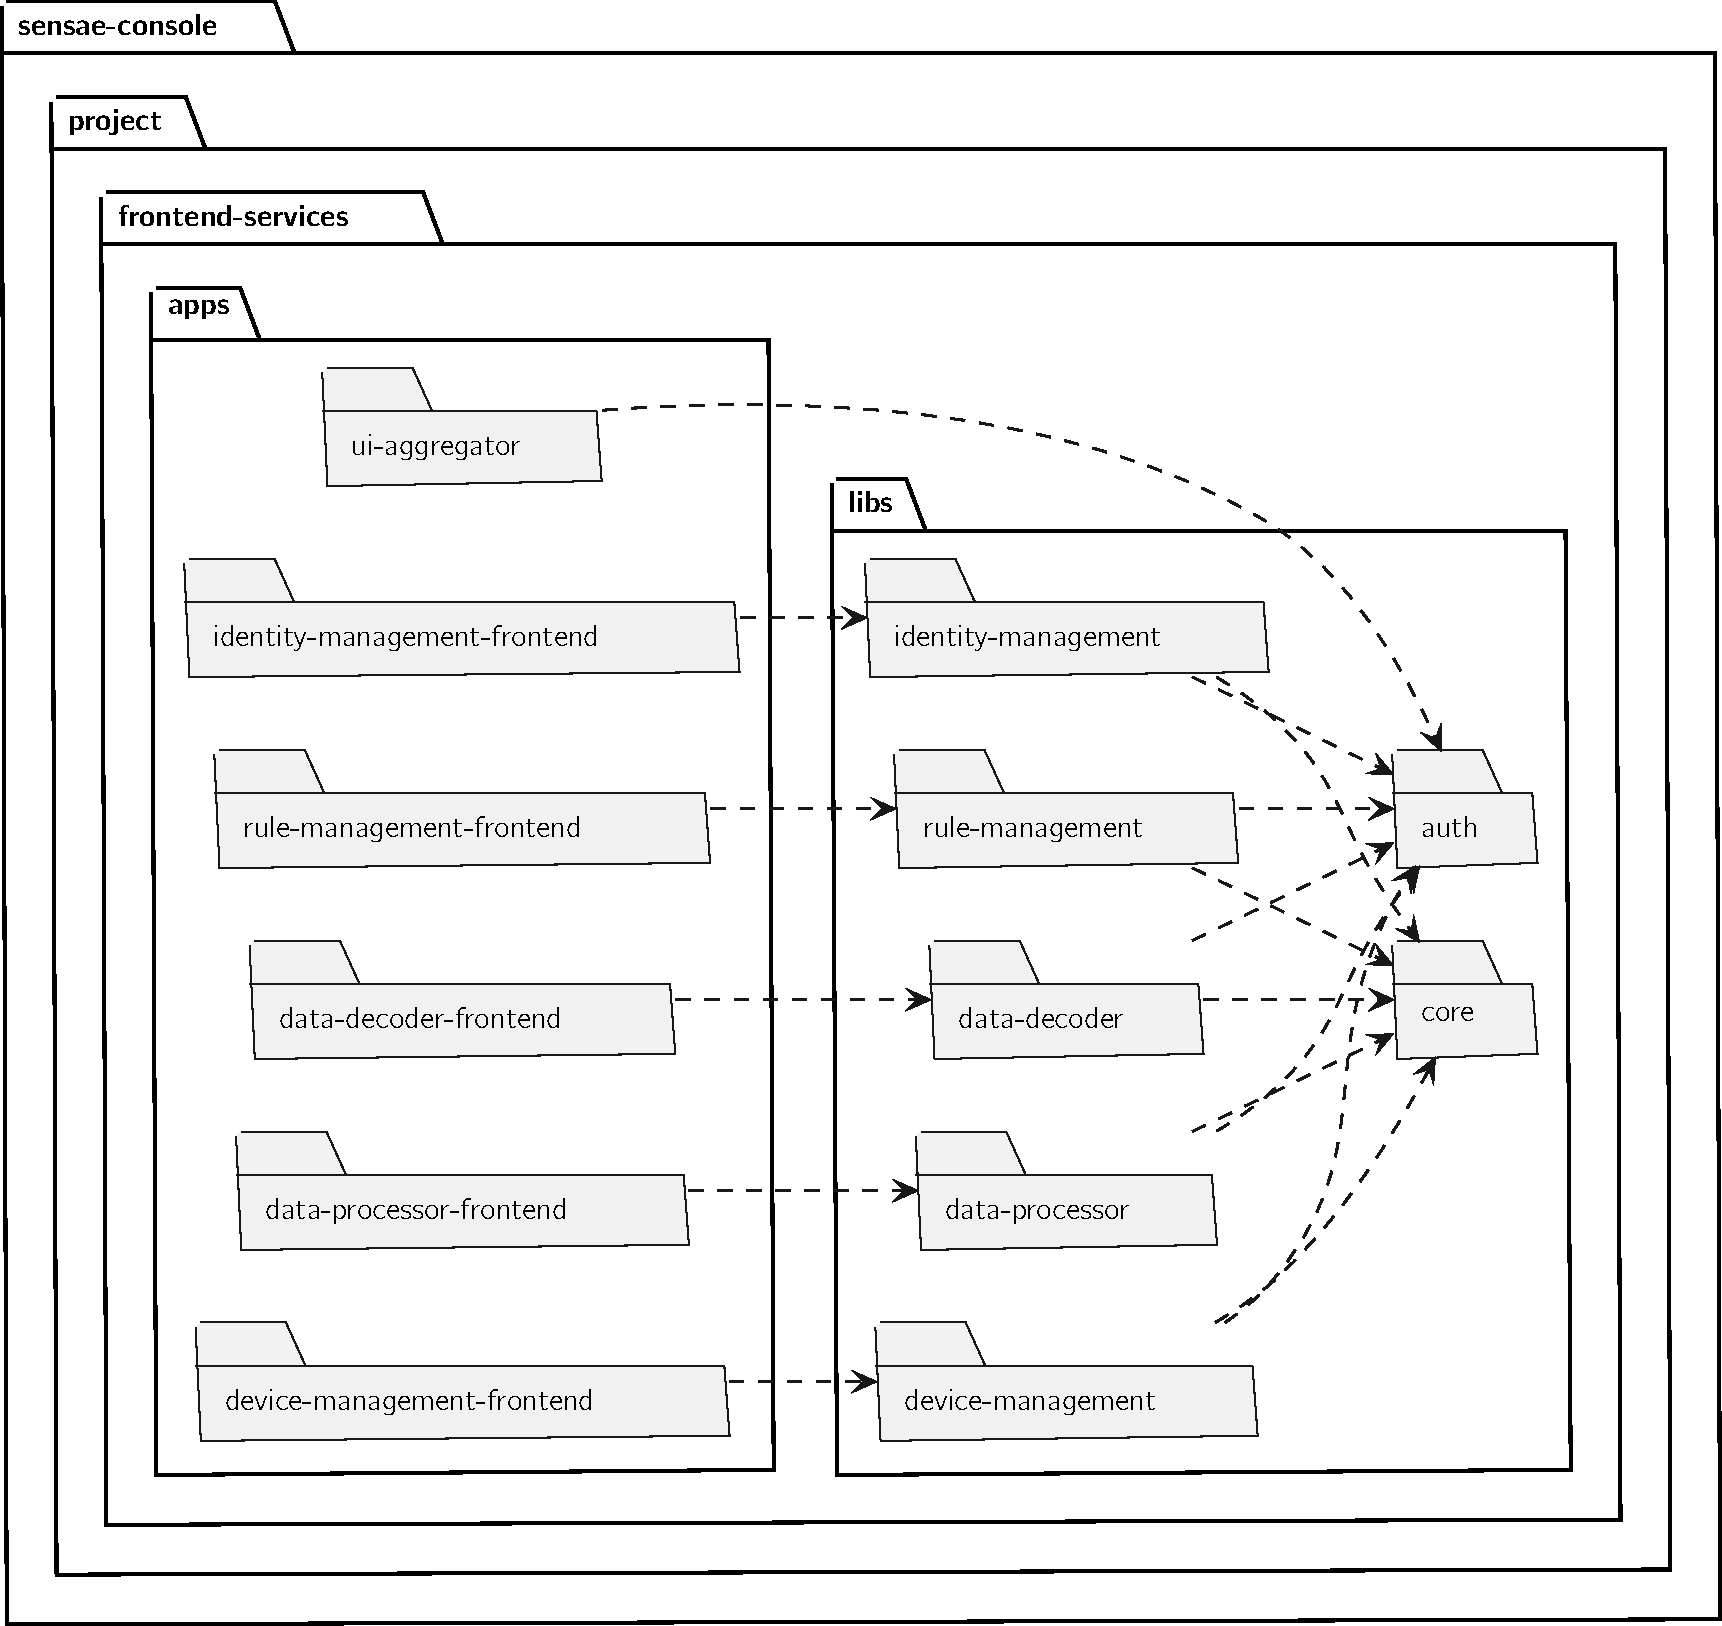
\includegraphics[page=1,width=\columnwidth]{assets/diagrams/design/architectural/level2/development/frontend.pdf}
   \caption[Frontend Services - Container Level - Implementation View Diagram]{Frontend Services - Container Level - Implementation View Diagram}
   \label{fig:design:architecture:platform:container:development:frontend}
\end{figure}

\subsubsection{Container Level - Physical View}
\label{par:design:architecture:platform:container:physical}

Next is the physical view, intended to familiarize the reader with the idealized production environment. Each container that composes the system is containerized via \textit{Docker} so that orchestration software like \textit{Docker Compose}, \textit{Docker Swarm}, \textit{Kubernetes} and \textit{OpenShift} can be used to ease the operation phase.

The production environment is orchestrated using \textit{Docker Compose} running in a single node/server. This decision was taken after acknowledging that currently there is no need to scale the solution, a single node has been capable of handling all throughput.  The Appendix~\ref{appendix:docker} details how this was implemented.

Each Container represented in Section~\ref{par:design:architecture:platform:container:logical} is mapped to a container in this view. Following the \citetitle{dbperservice}, each logical database also corresponds to a physical database.

As an example, the physical view of the Rule Management Concern is presented in Figure~\ref{fig:design:architecture:platform:container:physical:rule}. The complete Sensae Console solution is not presented for brevity reasons.

\begin{figure}[H]
   \centering
   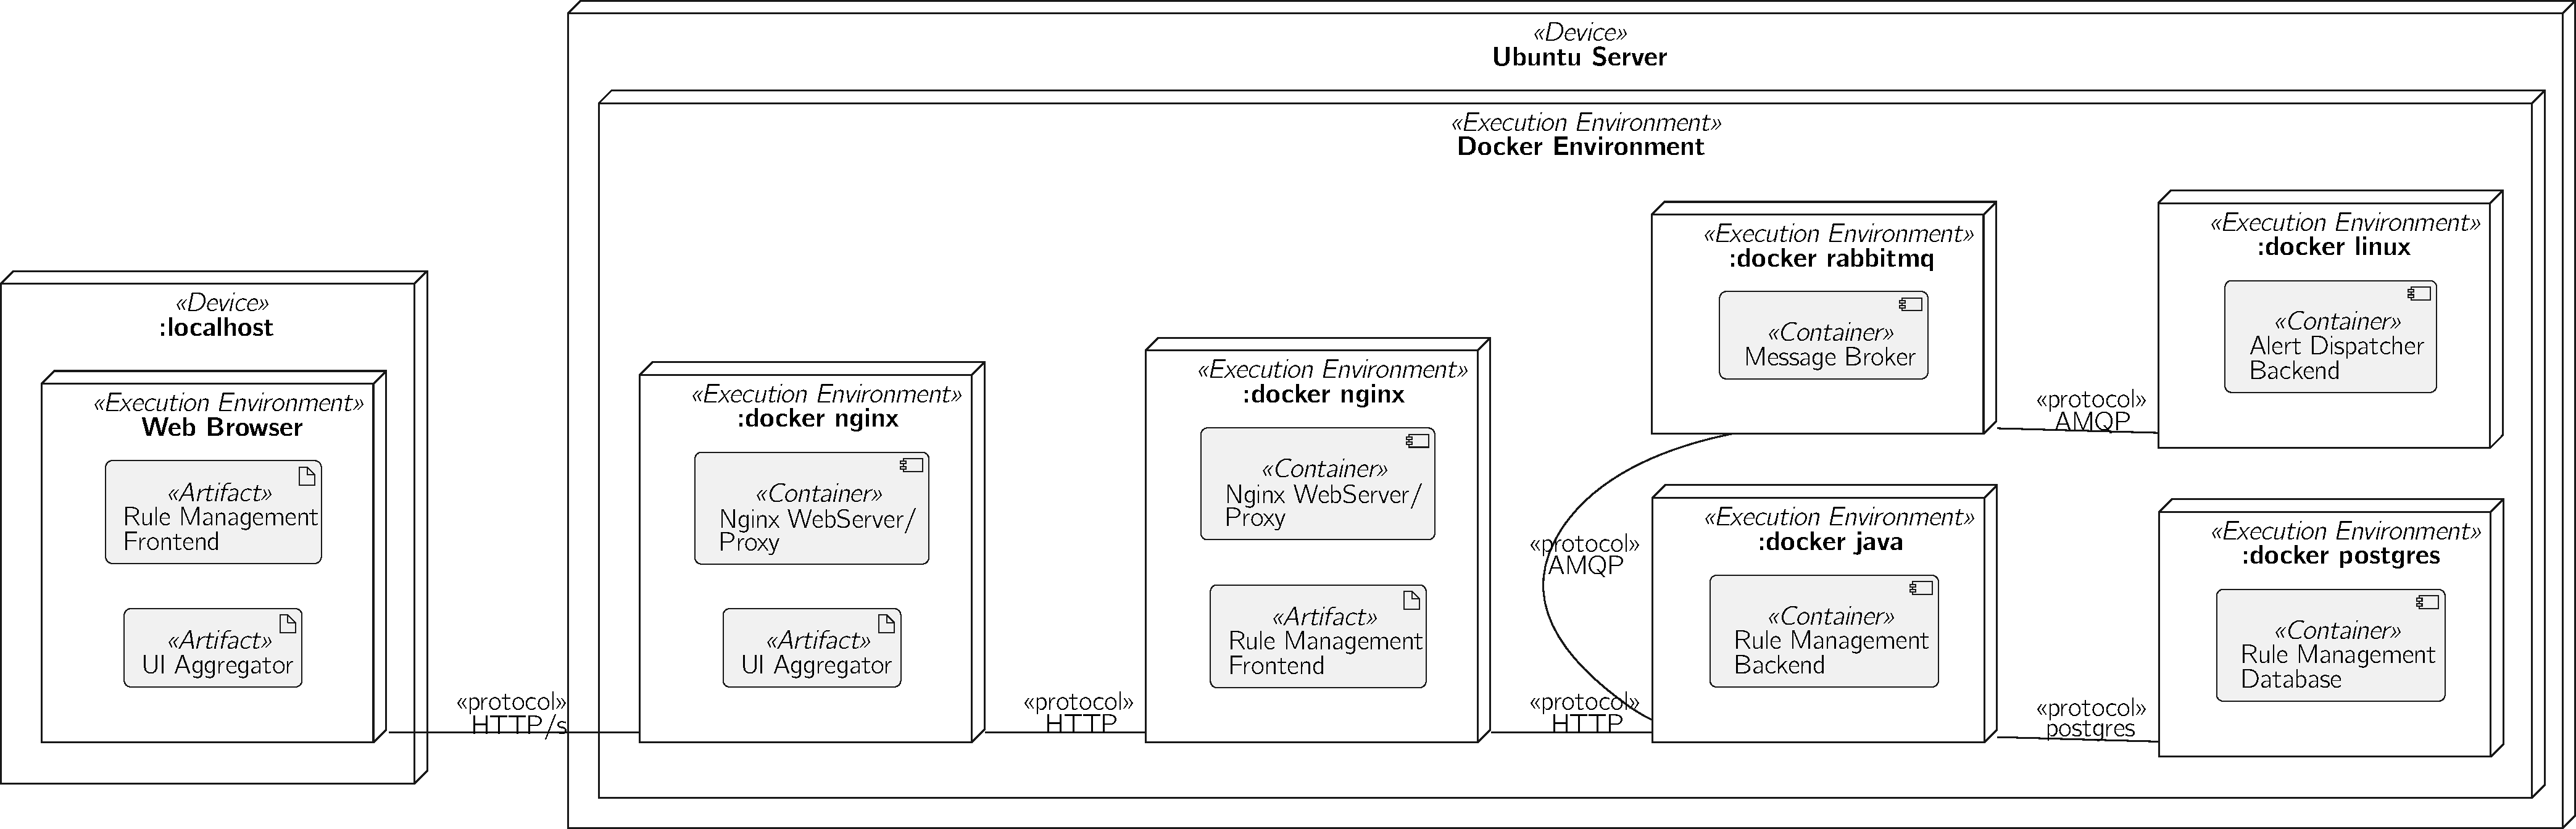
\includegraphics[page=1,width=\columnwidth]{assets/diagrams/design/architectural/level2/physical/rule-management-context.pdf}
   \caption[Rule Management - Container Level - Physical View Diagram]{Rule Management - Container Level - Physical View Diagram}
   \label{fig:design:architecture:platform:container:physical:rule}
\end{figure}

The two \textit{Device}s presented correspond to a user's machine (localhost) and the server where Sensae Console is deployed (Ubuntu Server). The \textbf{UI Aggregator} and \textbf{Rule Management Frontend} are served by their corresponding Nginx WebServer, and all user-centered communications with \textbf{Sensae Console} are secured and conducted by the UI Aggregator Nginx WebServer.

In the future, if the need arises, \textbf{Sensae Console} should be orchestrated with \textit{Kubernetes} or \textit{OpenShift}. This would allow the solution to auto-scale, multiplying the containers under excessive load.

\subsubsection{Container Level - Synopsis}
\label{par:design:architecture:platform:container:synopsis}

This section presented the \textbf{Sensae Console}'s C4 Level 2. Some concepts regarding how internal communication is achieved were introduced. The next section details these concepts.

\subsection{Canonical Model}
\label{sec:design:domain}

The idea behind this section is to introduce core communication concepts of \textbf{Sensae Console} to the reader. To represent these ideas the \gls{UML} notation is used. This section is presented here, after the \nameref{subsec:design:architecture:platform} Section to support some terms introduced there but not fully explained. It does not correspond to any C4 Model Level. 

The canonical model is comprised of concepts that transverse the entire \textbf{Sensae Console} business model, and by extension any \textbf{Business Application}. Therefore, it is built as a library, \textit{iot-core}, that can be used by entities that rely on the exchange of information with/inside \textbf{Sensae Console}. It can be seen as a domain that focus on defining the protocol of exchange of information between the various entities of the system.

The intent behind this model is to alleviate one of the issues related to distributed systems - heterogeneity in data formats \parencite{nadiminti2006distributed} - and to provide a simple \gls{SDK} for third-parties to develop new business applications that interact with \textbf{Sensae Console}. It can be seen as an explicit schema. According to \cite{explicitsharedmodel}, ``any implementation of event-based communication between a producer and consumer that lacks an explicit predefined schema will inevitably end up relying on an implicit schema. Implicit data contracts are brittle and susceptible to uncontrolled change, which can cause much undue hardship to downstream consumers.''

According to \cite{integration}, ``while we have historically drawn up our project plans and costs around the boxes — the digital products we are introducing — the lines are the hidden and often primary driver of organizational tech debt. They are the reason that things just take longer now than they used to.'' The \textit{'lines'} in this solution are a first class citizen and, instead of just linking the system together, they act as the pillars that shape the entire ecosystem.

It is comprised of three big components: (i) data model, (ii) message envelop model, and (iii) routing model.

The various domains inside \textbf{Sensae Console} and \textbf{Business Applications} are discussed in Appendix~\ref{appendix:design:domain:bounded_contexts} and \ref{appendix:design:domain:services_contexts}, respectively.

\subsubsection{Data Model}
\label{subsubsec:design:domain:shared_model:data}

The data model represents the \textbf{Data Unit} that \textbf{Sensae Console} is currently capable of understanding. The following diagram, Figure~\ref{fig:design:domain:shared_model:data:diagram}, is a high level specification.

\begin{figure}[H]
   \centering
   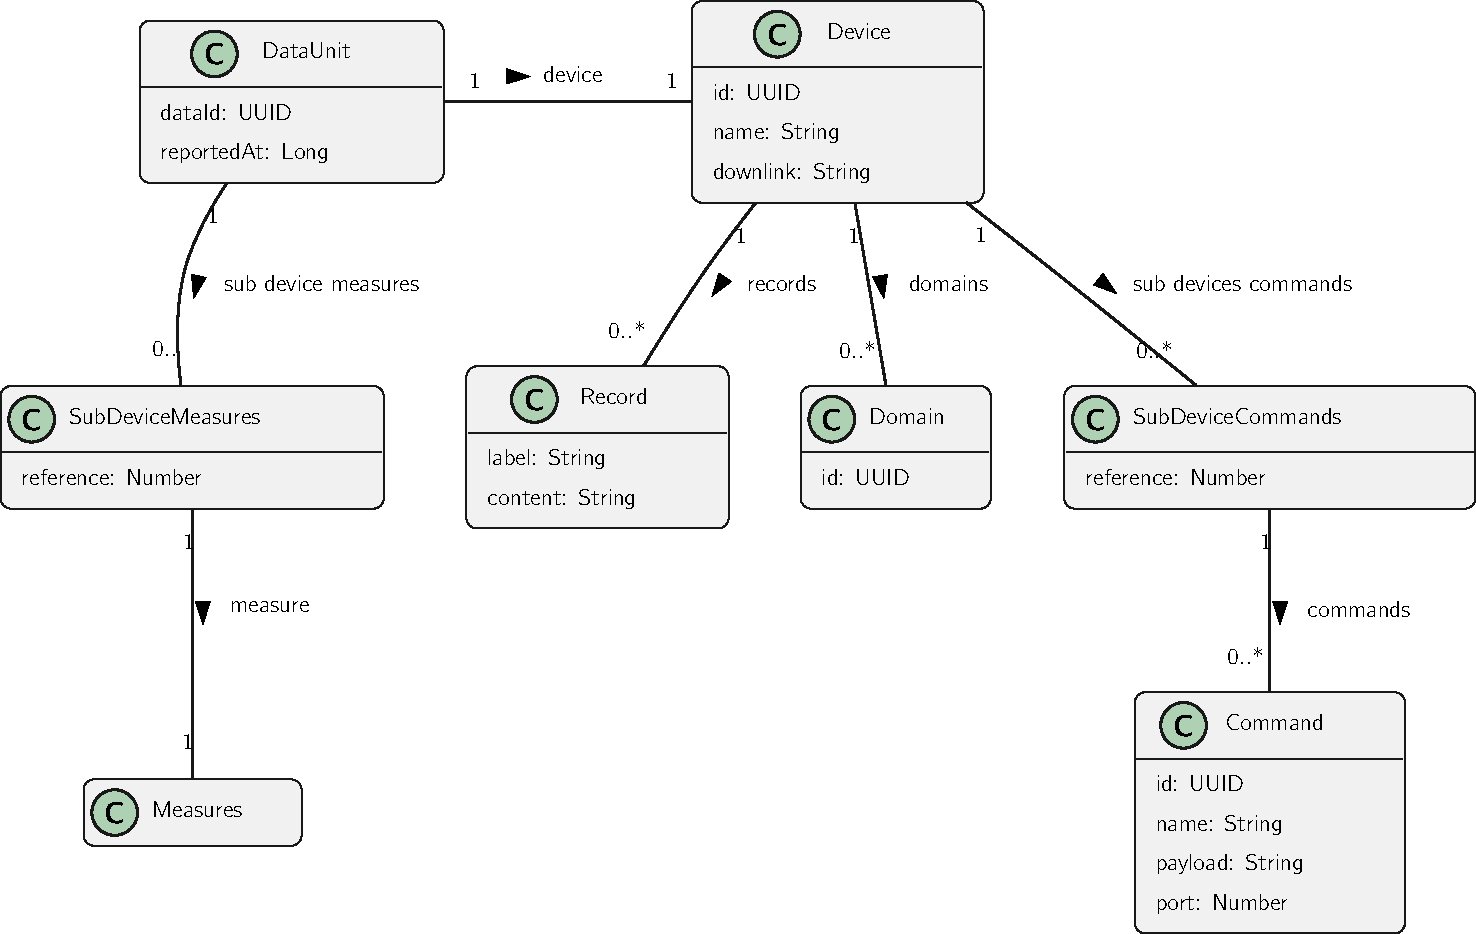
\includegraphics[page=1,width=\columnwidth]{assets/diagrams/design/domain/shared-model.pdf}
  \caption[Canonical Model - Data Unit]{Canonical Model - Data Unit}
  \label{fig:design:domain:shared_model:data:diagram}
\end{figure}

As a brief description of Figure~\ref{fig:design:domain:shared_model:data:diagram}:

\begin{itemize}
   \item \textbf{Data Unit} is the entry point to the shared model;
   \item The \textit{reportedAt} attribute represents an absolute timestamp of when the \textbf{Data Unit} was captured, in milliseconds;
   \item The \textit{Device} concept represents the \textbf{Device} that sent the \textit{Data Unit};
   \item The \textit{Record} concept represents an entry of \textbf{Records/Metadata};
   \item The \textit{Domain} concept references the \textbf{Domain} that owns the \textit{Device};
   \item The \textit{SubDeviceMeasures} referes to the collected measures. When the device is a Controller there's a need to map each sub device's measures with it and not with the Controller that sent the uplink. The \textit{reference} attribute indicates what sub device collected the measure, the reference \textit{zero} referes to the device that sent the uplink;
   \item The \textit{SubDeviceCommands} referes to the available commands to control the device. When the device is a Controller there's a need to map each sub device commands with it and not with the Controller that sent the uplink. The \textit{reference} attribute indicates the sub device that is controlled by the commands mentioned, the reference \textit{zero} referes to the device that sent the uplink;
   \item The \textit{Measures} concept contains various common data types related to \gls{IoT}.
\end{itemize}

As explained, \textit{Measures} contains various data types. Currently the supported types are presented in the Table~\ref{tab:design:domain:shared_model:data:data_types}. The team involved in this project decided what data types were needed to support based on the requested \gls{PoC}s and the purchased sensors. In the future more data types are expected to be included in the model.

The full json-like model schema can be found in Appendix~\ref{AppendixA}.

\begin{landscape}
   \begin{longtable}{cllll}
   \caption{Measure Data Types}
   \label{tab:design:domain:shared_model:data:data_types}\\
   \cline{1-4}
   \multicolumn{2}{l}{\textbf{Data Type}}                                     & \multirow{2}{*}{\textbf{Description}}                  & \multirow{2}{*}{\textbf{Unit}} &  \\
   \textit{Property}                     & \textit{Sub Property}              &                                                        &                                &  \\ \cline{1-4}
   \endfirsthead
   %
   \multicolumn{5}{c}%
   {{\bfseries Table \thetable\ continued from previous page}} \\
   \cline{1-4}
   \multicolumn{2}{l}{\textbf{Data Type}}                                     & \multirow{2}{*}{\textbf{Description}}                  & \multirow{2}{*}{\textbf{Unit}} &  \\
   \textit{Property}                     & \textit{Sub Property}              &                                                        &                                &  \\ \cline{1-4}
   \endhead
   %
   \\
   \cline{1-4}
   \\
   \endfoot
   %
   \endlastfoot
   %
   \\[-0.85em]
   \multicolumn{2}{l}{\textbf{Trigger}}                                       & \multicolumn{2}{l}{Type related to something with an on / off or open / close state}    &  \\
   \textit{trigger}                      & \textit{value}                     & Value can be true or false                                    & boolean                        &  \\ [0.4em] \cline{1-4}
   \\[-0.85em]
   \multicolumn{2}{l}{\textbf{Motion}}                                        & \multicolumn{2}{l}{Status related to the motion of a device}                            &  \\
   \textit{motion}                       & \textit{value}                     & Value can be "ACTIVE", "INACTIVE" or "UNKNOWN"         & n.a.                           &  \\ [0.4em] \cline{1-4}
   \\[-0.85em]
   \multicolumn{2}{l}{\textbf{Velocity}}                                      & \multicolumn{2}{l}{How fast a device is moving}                                         &  \\
   \textit{velocity}                     & \textit{kilometerPerHour}          & Value measured in                                      & km/h                           &  \\ [0.4em] \cline{1-4}
   \\[-0.85em]
   \multicolumn{2}{l}{\textbf{Temperature}}                                   & \multicolumn{2}{l}{Temperature measured by a device}                                    &  \\
   \textit{temperature}                  & \textit{celsius}                   & Value measured in                                      & celsius                        &  \\ [0.4em] \cline{1-4}
   \\[-0.85em]
   \multicolumn{2}{l}{\textbf{AQI}}                                           & \multicolumn{2}{l}{Air Quality Index according to the U.S. AQI}                         &  \\
   \textit{aqi}                          & \textit{value}                     & Value measured in                                      & AQI                            &  \\ [0.4em] \cline{1-4}
   \\[-0.85em]
   \multicolumn{2}{l}{\textbf{Air Pressure}}                                  & \multicolumn{2}{l}{Pressure within the atmosphere of Earth}                             &  \\
   \textit{airPressure}                  & \textit{hectoPascal}               & Value measured in                                      & hPa                            &  \\ [0.4em] \cline{1-4}
   \\[-0.85em]
   \multicolumn{2}{l}{\textbf{Distance}}                                      & \multicolumn{2}{l}{Distance measured from the device to a surface}                      &  \\
   \multirow{3}{*}{\textit{distance}}    & \textit{millimeters}               & Value measured in                                      & mm                             &  \\
                                         & \textit{maxMillimeters}            & Maximum distance the sensor can be to a given surface  & mm                             &  \\
                                         & \textit{minMillimeters}            & Minimum distance the sensor can be to a given surface  & mm                             &  \\ [0.4em] \cline{1-4}
   \\[-0.85em]
   \multicolumn{2}{l}{\textbf{Soil Moisture}}                                 & \multicolumn{2}{l}{Amount of water, including water vapor, in an unsaturated soil}      &  \\
   \textit{soilMoisture}                  & \textit{relativePercentage}        & Value measured in                                      & \%                             &  \\ [0.4em] \cline{1-4}
   \\[-0.85em]
   \multicolumn{2}{l}{\textbf{Water Pressure}}                                & \multicolumn{2}{l}{Water Pressure measured in pipes by a device}                        &  \\
   \textit{waterPressure}                & \textit{bar}                       & Value measured in                                      & bar                            &  \\ [0.4em] \cline{1-4}
   %\pagebreak
   \\[-0.85em]
   \multicolumn{2}{l}{\textbf{Illuminance}}                                   & \multicolumn{2}{l}{Illuminance level - luminous flux per unit area}                     &  \\
   \textit{illuminance}                  & \textit{lux}                       & Value measured in                                      & lux                            &  \\ [0.4em] \cline{1-4}
   \\[-0.85em]
   \multicolumn{2}{l}{\textbf{CO2}}                                           & \multicolumn{2}{l}{Atmospheric Carbon Dioxide concentration}                            &  \\
   \textit{co2}                          & \textit{ppm}                       & Value measured in                                      & ppm                            &  \\ [0.4em] \cline{1-4}
   \\[-0.85em]
   \multicolumn{2}{l}{\textbf{CO}}                                            & \multicolumn{2}{l}{Atmospheric Carbon Oxide concentration}                              &  \\
   \textit{co}                           & \textit{ppm}                       & Value measured in                                      & ppm                            &  \\ [0.4em] \cline{1-4}
   \\[-0.85em]
   \multicolumn{2}{l}{\textbf{VOC}}                                           & \multicolumn{2}{l}{Volatile Organic Compounds concentration measured by a device}       &  \\
   \textit{voc}                          & \textit{ppm}                       & Value measured in                                      & ppm                            &  \\ [0.4em] \cline{1-4}
   \\[-0.85em]
   \multicolumn{2}{l}{\textbf{NH3}}                                           & \multicolumn{2}{l}{Atmospheric Ammonia concentration}                                   &  \\
   \textit{nh3}                          & \textit{ppm}                       & Value measured in                                      & ppm                            &  \\ [0.4em] \cline{1-4}
   \\[-0.85em]
   \multicolumn{2}{l}{\textbf{O3}}                                            & \multicolumn{2}{l}{Atmospheric Ozone concentration measured by a device}                &  \\
   \textit{o3}                           & \textit{ppm}                       & Value measured in                                      & ppm                            &  \\ [0.4em] \cline{1-4}
   \\[-0.85em]
   \multicolumn{2}{l}{\textbf{NO2}}                                           & \multicolumn{2}{l}{Atmospheric Nitrogen dioxide concentration}                          &  \\
   \textit{no2}                          & \textit{ppm}                       & Value measured in                                      & ppm                            &  \\ [0.4em] \cline{1-4}
   \\[-0.85em]
   \multicolumn{2}{l}{\textbf{PM2.5}}                                         & \multicolumn{2}{l}{Particulate Matter in the air (size up to 2.5 micrometers)}          &  \\
   \textit{pm2\_5}                       & \textit{microGramsPerCubicMeter}   & Value measured in                                      & $\mu$g/m3                      &  \\ [0.4em] \cline{1-4}
   \\[-0.85em]
   \multicolumn{2}{l}{\textbf{PM10}}                                          & \multicolumn{2}{l}{Particulate Matter in the air (size up to 10 micrometers)}           &  \\
   \textit{pm10}                         & \textit{microGramsPerCubicMeter}   & Value measured in                                      & $\mu$g/m3                      &  \\ [0.4em] \cline{1-4}
   \\[-0.85em]
   \multicolumn{2}{l}{\textbf{pH}}                                            & \multicolumn{2}{l}{Scale used to specify how acidic or basic a water-based solution is} &  \\
   \textit{ph}                           & \textit{value}                     & Value between 0 and 14 measured in                     & pH                             &  \\ [0.4em] \cline{1-4}
   \\[-0.85em]
   \multicolumn{2}{l}{\textbf{Occupation}}                                    & Occupation percentage measured inside a vessel         &                                &  \\
   \textit{occupation}                   & \textit{percentage}                & Value measured in                                      & \%                             &  \\ [0.4em] \cline{1-4}
   \\[-0.85em]
   \multicolumn{2}{l}{\textbf{Soil Conductivity}}                             & \multicolumn{2}{l}{Substances ability to conduct an electrical current in the soil}     &  \\
   \textit{soilConductivity}             & \textit{microSiemensPerCentimeter} & Value measured in                                      & $\mu$S/cm                      &  \\ [0.4em] \cline{1-4}
   \\[-0.85em]
   \multicolumn{2}{l}{\textbf{Air Humidity}}                                  & \multicolumn{2}{l}{Concentration of water vapour present in the air}                    &  \\
   \multirow{2}{*}{\textit{airHumidity}} & \textit{gramsPerCubicMeter}        & Value measured in                                      & g/m3                           &  \\
                                         & \textit{relativePercentage}        & Value measured in                                      & \%                             &  \\ [0.4em] \cline{1-4}
   \\[-0.85em]
   \multicolumn{2}{l}{\textbf{GPS}}                                           & \multicolumn{2}{l}{Point reference in the Geographic Coordinate System}                 &  \\
   \multirow{3}{*}{\textit{gps}}         & \textit{latitude}                  & Value between -90 and 90 measured in                   & degrees                        &  \\
                                         & \textit{longitude}                 & Value between -180 and 180 measured in                 & degrees                        &  \\
                                         & \textit{altitude}                  & Value determined according to the mean sea level       & meters                         &  \\ [0.4em] \cline{1-4}
   \\[-0.85em]
   \multicolumn{2}{l}{\textbf{Battery}}                                       & \multicolumn{2}{l}{Battery of the device}                                               &  \\
   \multirow{4}{*}{\textit{battery}}     & \textit{volts}                     & Value measured in                                      & volts                          &  \\
                                         & \textit{percentage}                & Value measured in                                      & \%                             &  \\
                                         & \textit{maxVolts}                  & Minimum volts the battery needs for the device to work & volts                          &  \\
                                         & \textit{minVolts}                  & Maximum volts the battery can hold                     & volts                          &  \\ [0.4em] \cline{1-4}
   \end{longtable}
\end{landscape}

\subsubsection{Message Envelop Model}
\label{subsubsec:design:domain:shared_model:message}

The message envelop model refers to how, coupled with the routing model in Section~\ref{subsubsec:design:domain:shared_model:routing}, information can reliably transverse the system.

The diagram present in Figure~\ref{fig:design:domain:shared_model:messsage:diagram} details this model.

\begin{figure}[H]
   \centering
   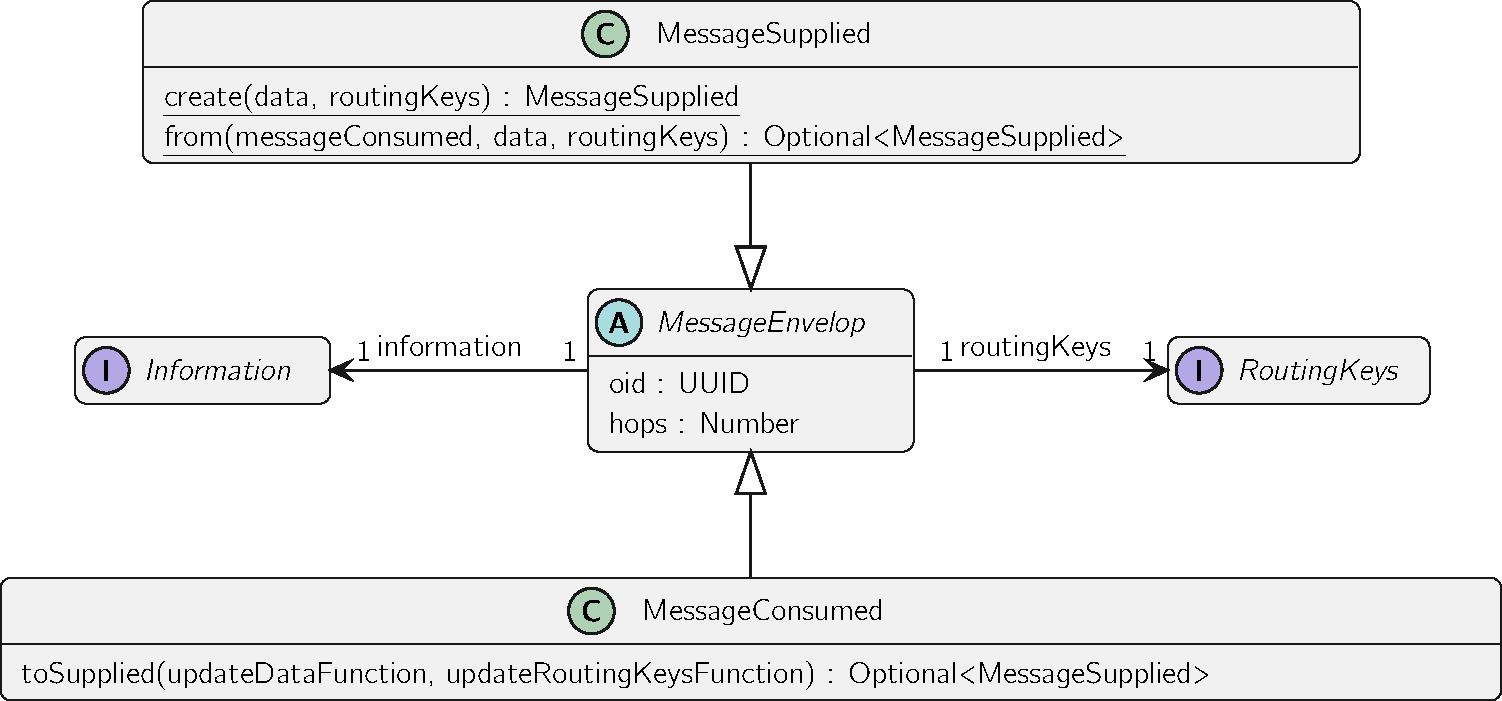
\includegraphics[page=1,width=0.8\columnwidth]{assets/diagrams/design/domain/message-envelop-model.pdf}
  \caption[Canonical Model - Message Envelop Model]{Canonical Model - Message Envelop Model}
  \label{fig:design:domain:shared_model:messsage:diagram}
\end{figure}

As a brief description of Figure~\ref{fig:design:domain:shared_model:messsage:diagram}:

\begin{itemize}
   \item A \textit{MessageSupplied} is created in a issuer system and supplied to start the flow of information in the system;
   \item A \textit{MessageConsumed} is consumed by a consumer system and can then be transformed into a \textit{MessageSupplied} to be supplied;
   \item \textit{Information} represents the content of the message;
   \item \textit{RoutingKeys} represents the model referenced in Section~\ref{subsubsec:design:domain:shared_model:routing};
\end{itemize}

This concept is mainly used to ensure that information flowing in the system is not reprocessed, by verifying the unique id - \textit{oid}, and is eliminated if it enters a routing loop by verifying that the \textit{hops} have not reached a maximum value.

\subsubsection{Routing Model}
\label{subsubsec:design:domain:shared_model:routing}

The routing model refers to how information can be routed through the system based on various parameters. The current idea is based on the \textit{pub/sub} pattern, as discussed by \cite{urquhart2021flow}. Containers subscribe to information in a \textbf{Topic} with specific \textit{RoutingKey}s and publish information with \textit{RoutingKey}s.

The diagram presented in Figure~\ref{fig:design:domain:shared_model:routing:diagram} details this model.

\begin{figure}[H]
   \centering
  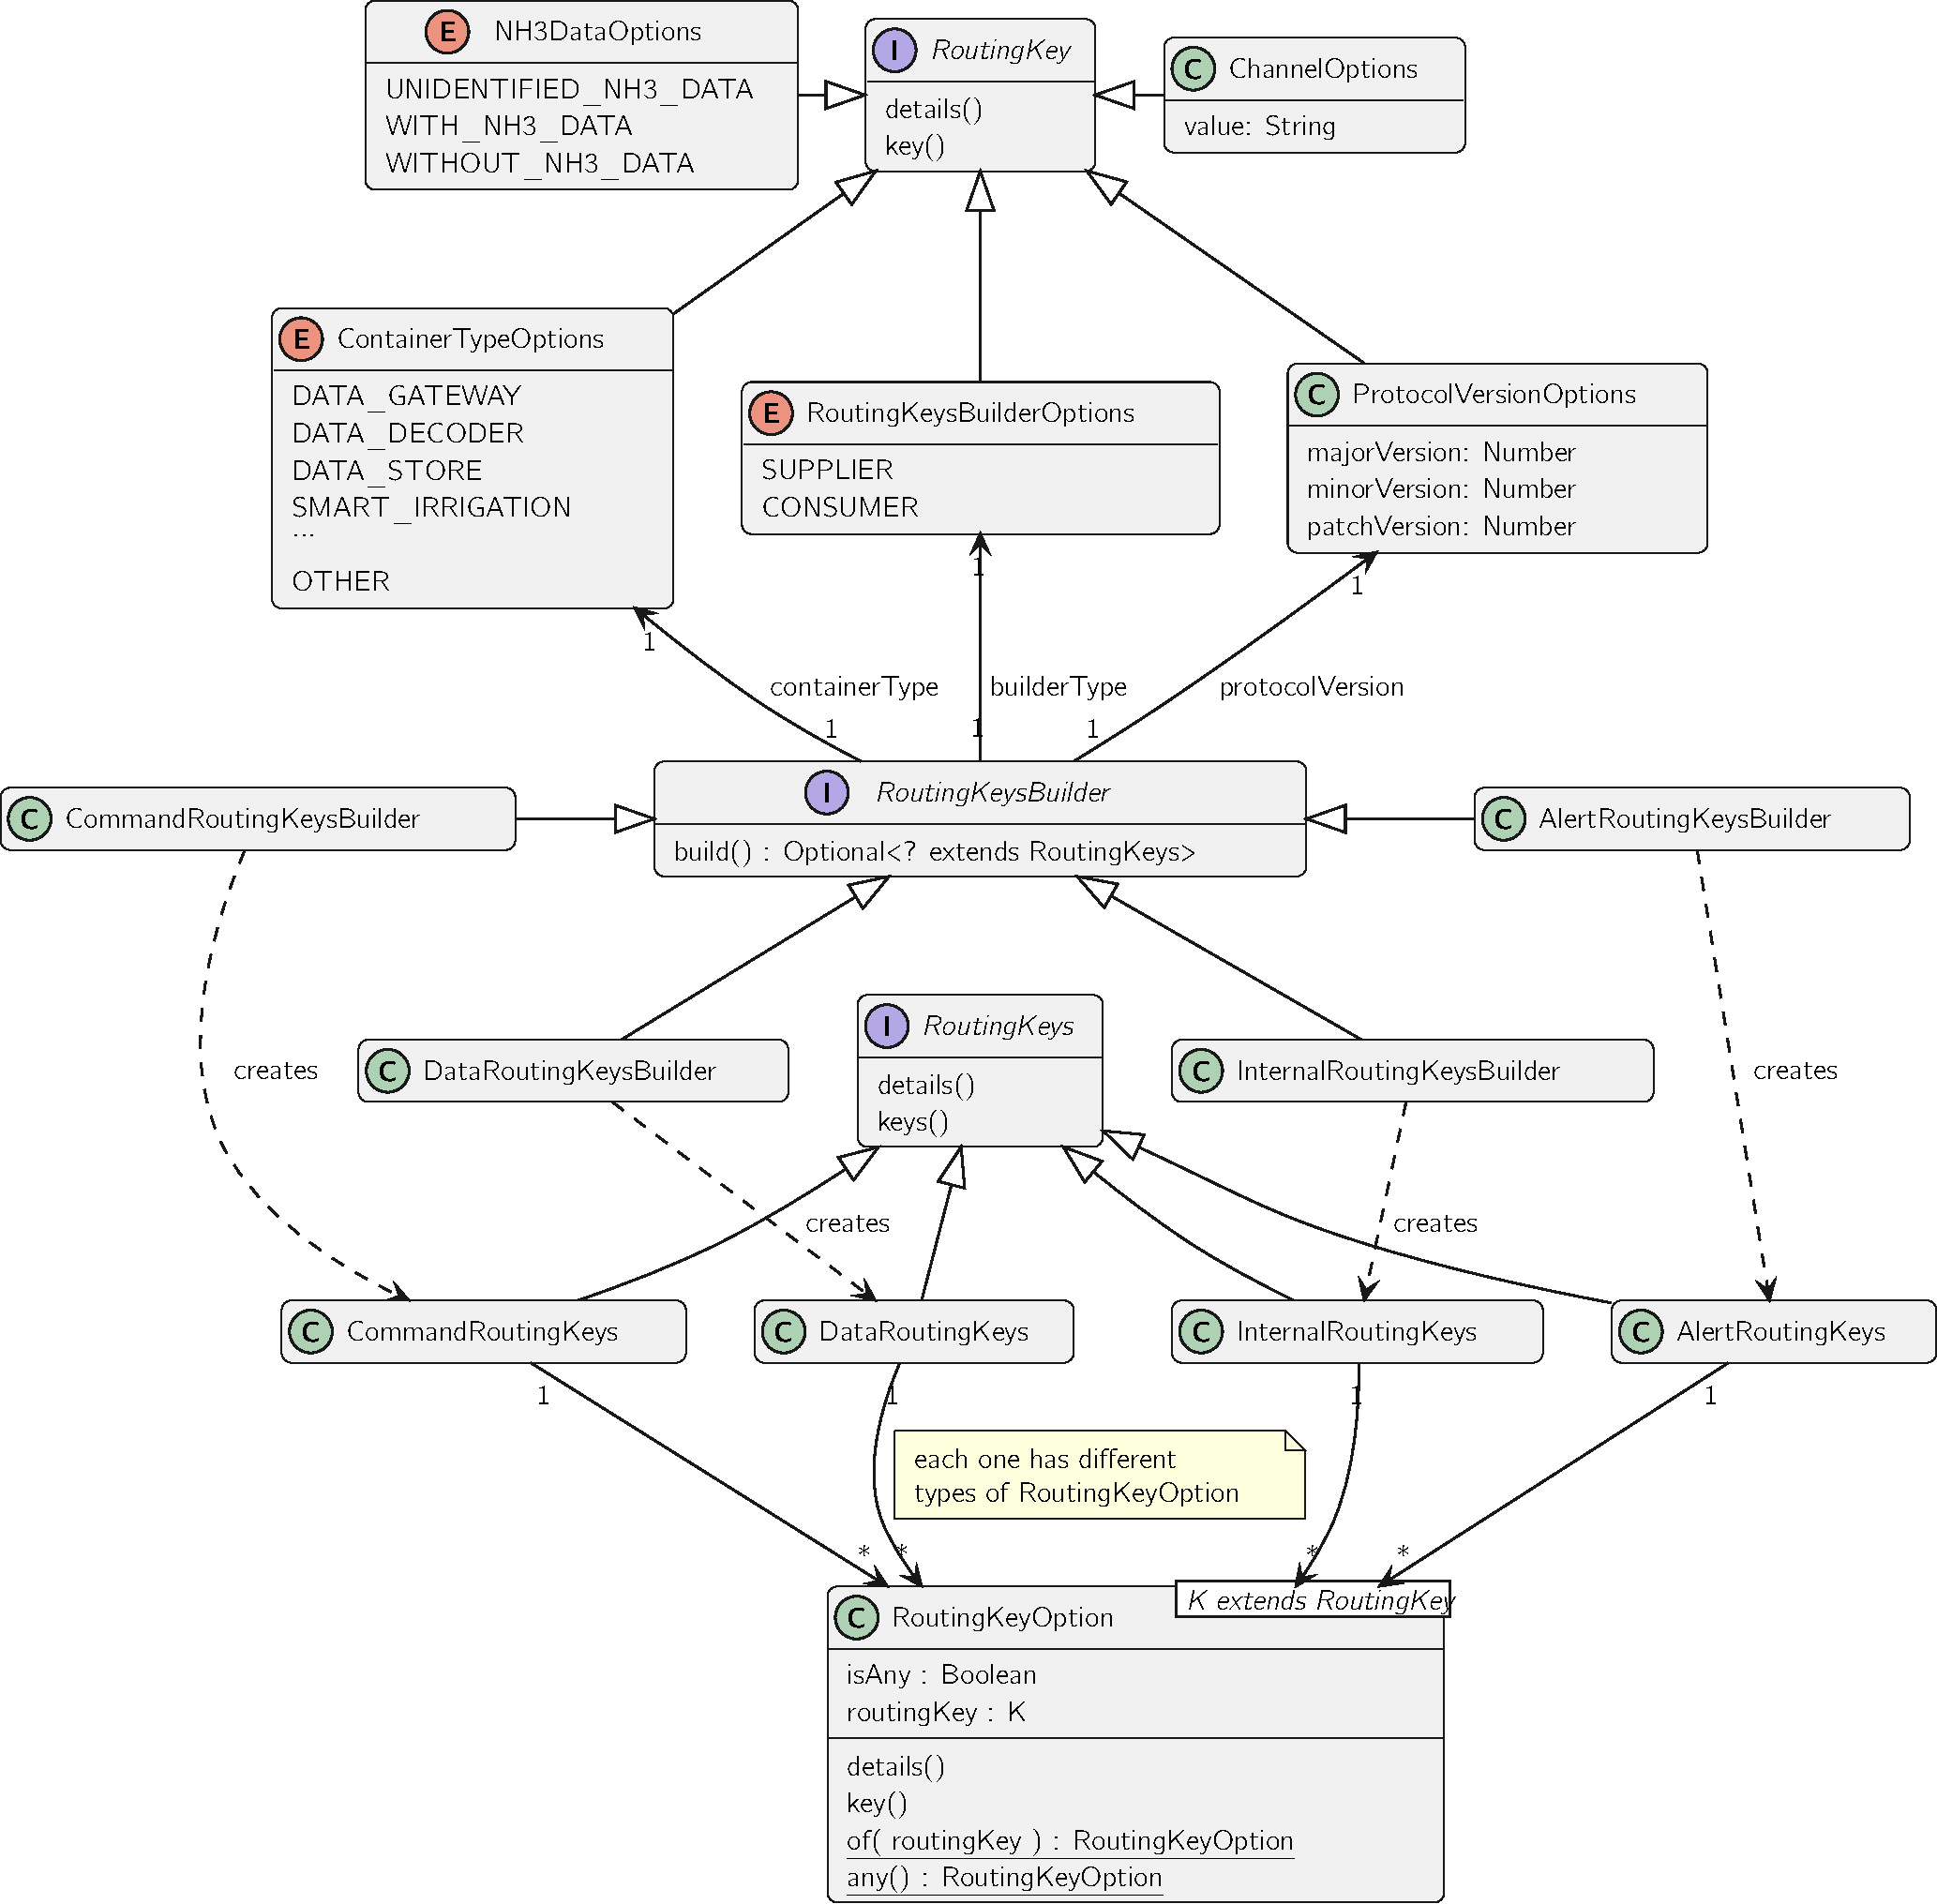
\includegraphics[page=1,width=\columnwidth]{assets/diagrams/design/domain/routing-model.pdf}
  \caption[Canonical Model - Routing]{Canonical Model - Routing}
  \label{fig:design:domain:shared_model:routing:diagram}
\end{figure}

As a brief description of Figure~\ref{fig:design:domain:shared_model:routing:diagram}:

\begin{itemize}
   \item \textit{RoutingKeys} is the concept referenced in Figure~\ref{fig:design:domain:shared_model:messsage:diagram} and represents a collection of different \textit{RoutingKeyOption}s;
   \item There are 4 types of \textit{RoutingKeys}, one for each \textbf{Topic} (according to \nameref{subsec:design:domain:taxonomy});
   \item To ensure that the various containers in \textbf{Sensae Console} understand each other, a \textit{ProtocolVersionOptions} is provided. This concept follows the Semantic Versioning Specification 2.0 \parencite{semver} an is assembled according to the version of \textit{iot-core} imported by the container;
   \item There are multiple \textit{RoutingKey} types not displayed in the diagram for brevity;
   \item A \textit{RoutingKeyOption} can have the value \textit{any}, if the \textit{RoutingKeysBuilderOptions} has the value \textit{CONSUMER}. This provides a 'relaxed' mode, for containers that consume/subscribe to messages and a 'strict' mode, where all \textit{RoutingKey} must be specified, for containers that supply/publish messages;
   \item The \textit{RoutingKeysBuilder} implements the \textit{Builder} pattern and its single responsibility is to validate and create \textit{RoutingKeys};
   \item \textit{NH3DataOptions} and \textit{ChannelOptions} are two examples of \textit{RoutingKey}, both used in the Data Topic.
\end{itemize}

Table~\ref{tab:design:domain:shared_model:routing} presents all currently used \textit{RoutingKey}s.

The routing key \textit{OperationType} from the \textbf{Internal} topic can have the following values:

\begin{itemize}
   \item \textbf{Sync}: message contains the current state of the related \textit{ContextType}, used to populate a container's state;
   \item \textbf{Info}: message contains information about an entry of the related \textit{ContextType}, e.g. entry X in context Y was removed;
   \item \textbf{Unknown}: message contains entry of the related \textit{ContextType} that the container that published the message can't identify;
   \item \textbf{Init}: message to notify that a container has initiated and needs the current state of the related \textit{ContextType} to be ready;
   \item \textbf{Ping}: message to notify that an entry of the related \textit{ContextType} was used, e.g. entry X in context Y was just used.
\end{itemize}

The \textit{ContextType}in Table~\ref{tab:design:domain:shared_model:routing}, used to identity what piece of the state is referenced, can currently have the following values: (i) \textit{Data Processor}, (ii) \textit{Data Decoder}, (iii) \textit{Device Information}, (iv) \textit{Device Identity}, (v) \textit{Tenant Identity}, and (vi) \textit{Rule Management}.

Routing keys help to strengthen the boundaries that a container is expected to have. As an example, a business application related to Waste Management would subscribe to the \textit{Data Topic} with the following \textit{Routing Keys}:

\begin{itemize}
   \item \textit{Info Type Options}: PROCESSED;
   \item \textit{Channel Options}: 'wasteManagement';
   \item \textit{Data Legitimacy Options}: CORRECT;
   \item \textit{GPS Data Options}: WITH;
   \item \textit{Occupation Data Options}: WITH;
   \item \textit{Records Options}: WITH;
   \item \textit{Ownership Options}: WITH.
\end{itemize}

And would, for example, subscribe to the \textit{Alert Topic} with the following \textit{Routing Keys}:

\begin{itemize}
   \item \textit{Alert Category Options}: 'wasteManagement';
   \item \textit{Alert SubCategory Options}: 'garbageFull';
   \item \textit{Ownership Options}: WITH.
\end{itemize}

As expected, the structure and semantics of the information subscribed to are known upfront with the help of the package \textit{iot-core}. The services developed and their pre-defined boundaries regarding data types consumed are detailed in Section~\ref{subsec:implementation:description:services}.

\begin{landscape}
   \begin{longtable}{cll}
   \caption{Routing Options}
   \label{tab:design:domain:shared_model:routing}\\
   \cline{1-2}
   \multicolumn{1}{l}{\textbf{Topic}}      & \multirow{2}{*}{\textbf{Description}}                                                                     &  \\
   \textit{Routing Key}                    &                                                                                                           &  \\ \cline{1-2}
   \endfirsthead
   %
   \multicolumn{3}{c}%
   {{\bfseries Table \thetable\ continued from previous page}} \\
   \cline{1-2}
   \multicolumn{1}{l}{\textbf{Topic}}      & \multirow{2}{*}{\textbf{Description}}                                                                     &  \\
   \textit{Routing Key}                    &                                                                                                           &  \\ \cline{1-2}
   \endhead
   %
   \cline{1-2}
   \endfoot
   %
   \endlastfoot
   %
   \multicolumn{1}{l}{\textbf{Common}}     & Routing Keys that belong to every Topic                                                                   &  \\
   \textit{Protocol Version Options}       & Version of the used \textit{iot-core} package                                                             &  \\
   \textit{Container Type Options}         & Type of the Container that published the message                                                          &  \\
   \textit{Ownership Options}              & Does the message contains the \textbf{Domain}s that own it\footnotemark[1]                                &  \\
   \textit{Topic Type Options}             & Topic used to publish the message                                                                         &  \\ \cline{1-2}
   \multicolumn{1}{l}{\textbf{Internal}}   & Routing Keys that belong to the Internal Topic                                                            &  \\
   \textit{Operation Type Options}         & Intent of the message, e.g. unknown context found                                                         &  \\
   \textit{Context Type Options}           & Type of content in the message, e.g. device information                                                   &  \\ \cline{1-2}
   \multicolumn{1}{l}{\textbf{Data}}       & Routing Keys that belong to the Data Topic                                                                &  \\
   \textit{Info Type Options}              & How data is shaped: (i) ENCODED, (ii) DECODED and (iii) PROCESSED                                         &  \\
   \textit{Device Type Options}            & Type of device, e.g. LGT-92 or EM300-TH                                                                   &  \\
   \textit{Channel Options}                & Name of channel where data flows, e.g. \textit{smartIrrigation} or \textit{default}                       &  \\
   \textit{Data Legitimacy Options}        & Is the data legitimate: (i) UNKNOWN, (ii) CORRECT, (iii) INCORRECT and (iv) UNDETERMINED      &  \\
   \textit{Records Options}                & Does the data contains \textbf{Records/Metadata}\footnotemark[1]                                          &  \\
   \textit{Air Humidity Data Options}      & Does the data contains information about Air Humidity\footnotemark[1]\footnotemark[2]                     &  \\
   \textit{Air Pressure Data Options}      & Does the data contains information about Air Pressure\footnotemark[1]\footnotemark[2]                     &  \\
   \textit{Air Quality Data Options}       & Does the data contains information about Air Quality\footnotemark[1]\footnotemark[2]                      &  \\
   \textit{Battery Data Options}           & Does the data contains information about the device Battery\footnotemark[1]\footnotemark[2]               &  \\
   \textit{CO2 Data Options}               & Does the data contains information about CO2 levels\footnotemark[1]\footnotemark[2]                       &  \\
   \textit{CO Data Options}                & Does the data contains information about CO levels\footnotemark[1]\footnotemark[2]                        &  \\
   \textit{Distance Data Options}          & Does the data contains information about distances to a surface\footnotemark[1]\footnotemark[2]           &  \\
   \textit{GPS Data Options}               & Does the data contains information about the device GPS coordinates\footnotemark[1]\footnotemark[2]       &  \\
   \textit{Illuminance Data Options}       & Does the data contains information about illuminance in the environment\footnotemark[1]\footnotemark[2]   &  \\
   \textit{Motion Data Options}            & Does the data contains information about the device motion\footnotemark[1]\footnotemark[2]                &  \\
   \textit{NH3 Data Options}               & Does the data contains information about NH3 levels\footnotemark[1]\footnotemark[2]                       &  \\
   \textit{NO2 Data Options}               & Does the data contains information about NO2 levels\footnotemark[1]\footnotemark[2]                       &  \\
   \textit{O3 Data Options}                & Does the data contains information about O3 levels\footnotemark[1]\footnotemark[2]                        &  \\
   \textit{Occupation Data Options}        & Does the data contains information about occupation levels\footnotemark[1]\footnotemark[2]                &  \\
   \textit{pH Data Options}                & Does the data contains information about ph level\footnotemark[1]\footnotemark[2]                         &  \\
   \textit{PM2.5 Data Options}             & Does the data contains information about pm 2.5 concentration\footnotemark[1]\footnotemark[2]             &  \\
   \textit{PM10 Data Options}              & Does the data contains information about pm 10 concentration\footnotemark[1]\footnotemark[2]              &  \\
   \textit{Soil Conductivity Data Options} & Does the data contains information about the soil conductivity\footnotemark[1]\footnotemark[2]            &  \\
   \textit{Soil Moisture Data Options}     & Does the data contains information about the soil moisture\footnotemark[1]\footnotemark[2]                &  \\
   \textit{Temperature Data Options}       & Does the data contains information about the temperature\footnotemark[1]\footnotemark[2]                  &  \\
   \textit{Trigger Data Options}           & Does the data contains information about something that works as a switch\footnotemark[1]\footnotemark[2] &  \\
   \textit{Velocity Data Options}          & Does the data contains information about the device velocity\footnotemark[1]\footnotemark[2]              &  \\
   \textit{VOC Data Options}               & Does the data contains information about VOC concentration\footnotemark[1]\footnotemark[2]                &  \\
   \textit{Water Pressure Data Options}    & Does the data contains information about water pressure\footnotemark[1]\footnotemark[2]                   &  \\ \cline{1-2}
   \multicolumn{1}{l}{\textbf{Command}}    & Routing Keys that belong to the Command Topic                                                             &  \\
   \textit{Command Type Options}           & Type of command, e.g. Open Valve                                                                          &  \\ \cline{1-2}
   \multicolumn{1}{l}{\textbf{Alert}}      & Routing Keys that belong to the Alert Topic                                                               &  \\
   \textit{Alert Category Options}         & Category of the alert published, e.g. Fire Detention                                                      &  \\
   \textit{Alert Subcategory Options}      & Category of the alert published, e.g. Humidity With High Rate Of Change                                   &  \\
   \textit{Alert Severity Options}         & Severity of the alert published, from \textit{Information} level to \textit{Critical} level               &  \\ \cline{1-2}
   \end{longtable}
   \footnotetext[1]{has three possible values: (i) UNDETERMINED, (ii) WITH, (iii) WITHOUT}
   \footnotetext[2]{related to the explored Data Types}
\end{landscape}

\subsection{Synopsis}
\label{subsubsec:design:architecture:synopsis}

This section discussed the architecture used in the platform. It presented how some internal processes are handled by the system as a whole with the help of the Canonical Model.
In the following section, alternatives to what was designed and developed across the system are discussed.

\section{Architectural Alternatives}
\label{sec:design:alternatives}

This section tackles important alternatives that were proposed and discussed during the design and development of the system but were discarded in detriment for the approaches presented in the \nameref{sec:design:architecture}.

More alternatives are discussed in the appendixes, namely User Authentication, in Appendix~\ref{appendix:design:alternatives:auth}.

\subsection{Backend Segregation}
\label{subsec:design:alternatives:backend}

There are three main architectural approaches to this topic: Monolithic Backend - \cite{micromono} -, \gls{SOA} - \cite{ibmsoa} - or Microservices - \cite{martinmicro}. The first question regarding what to choose is whether to split the system in multiple units of work: Monolith vs the other two approaches.

If the decision is to split the system, then an important question must be asked: how should one split the system? The system architecture depends on the answer given: a \gls{SOA} emphasizes the reuse of the system functionalities, \cite{ibmsoa}, while Micro Services emphasis the decoupling of the various system components - \cite{micromicro} - and can therefore introduce some functionality duplication as opposed to \gls{SOA} - \cite{soavsmicro}.

But, to pick one of this architectures, the most important question to ask is: Why do i need architecture \textit{X}? To answer this, a set of the concerns deemed more important, with regards to this solution requirements, are discussed:

\begin{itemize}
   \item Time To Market: a \gls{MVP} should be available and ready to use as soon as possible;
   \item Extensibility of the solution: it should be easy to extend the solution with new Business Applications;
   \item Operation Cost: the solution has to be efficient to lower the infrastructure costs, tied to the system performance;
   \item System performance: the solution has to be capable of processing high volumes of data efficiently, tied to the system performance.
\end{itemize}

The first concern, Time to Market, weights heavily in favor of the Monolith approach when developing a \gls{MVP}, \cite{atlassianmono}. This approach is simpler to develop, deploy and has less cognitive overhead when compared to the other two approaches.

Regarding the extensibility of the solution, a Monolith is inherently rigid and hard to extend as the business evolves. This problem is inflated by the fact that the business model envisioned relies heavily on the creation of several Business Applications. On the order hand the \gls{SOA} and Microservices architecture are preferred since, due to their inherently decoupled nature, they are easier to extend using the interfaces they expose - \cite{microsoftmicro}.

The last two concerns are related to the scalability of the solution. A Monolithic Backend can only be scaled up by increasing the resources - RAM, CPU, GPU and Dick Capacity - of the physical server where the solution is deployed, this is commonly referred as Vertical Scaling. A \gls{SOA} or Micro Service Backend Architecture, apart from the Vertical Scaling option, can also be scaled up by increasing the number of physical servers where the solution is deployed, this is commonly referred as Horizontal Scaling.

Another option, that can be used with any architecture, is to deploy various independent instances of the same solution. Each instance would be assign to a set of costumers. This option is crucial and always possible once the business grows and starts to assist various customers.

The following picture, Figure~\ref{fig:design:alternatives:auth:backend:scale}, summarizes how each architect scales, the \gls{SOA} behaves similarly to the microservices architecture presented.

\begin{figure}[H]
   \centering
   \resizebox{\columnwidth}{!}
   {
      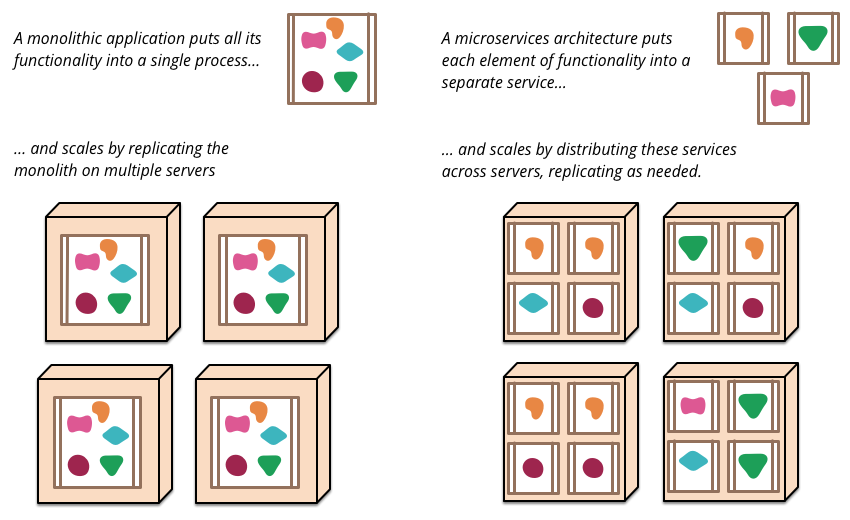
\includegraphics{assets/figures/microservices.png}
   }
   \caption[Monoliths and Microservices]{Monoliths and Microservices by \cite{martinmicro}}
   \label{fig:design:alternatives:auth:backend:scale}
\end{figure}

The final decision was to follow an architecture based on Microservices, even tho this decision had several oversights:

\begin{itemize}
   \item Development Team size: microservices are commonly adopted by big companies where each team of developers is responsible for a subset of microservices. This lowers the friction between teams when developing and deploying the solution and is seen as a big reason to move to a microservice architecture. For this solution, a single developer is responsible for everything;
   \item Time to Market: microservices need to interact with each other though the network. This added demand takes time to design and develop when compared to a monolith solution where communication is done via code;
   \item A solution shouldn't start with a microservice architecture: a solution should migrate to microservices when it becomes too complex and hard to maintain, \cite{ibmmicro}.
\end{itemize}

The decision made was based on the following assumptions, perceptions and findings:

\begin{itemize}
   \item There are well defined boundaries between the various business processes that the project needs to support;
   \item There is a perception that the solution will need to scale early on the road due to high volumes of \gls{IoT} data to process and store;
   \item There are a high number of completely independent business applications to develop and deploy;
   \item There are different types of costumers with diverse requirements regarding the deployment and development of the solution;
   \item Each costumer is interested in their specific business case or cases and therefore requires different combinations of business applications.
\end{itemize}

\gls{SOA} was discarded since: ``Although the concept of a share-as-much-as-possible architecture solves issues associated with the duplication of business functionality, it also tends to lead to tightly coupled components and increases the overall risk associated with change''. \parencite{richards2015microservices}. Microservices are more easily extended when/if needed compared with \gls{SOA} since the focus is on loose coupling services and not highly reusable services.

Despite this, the solution adopted some architecture decisions that are usually associated with \gls{SOA}, as an example a canonical data model (Section~\ref{sec:design:domain}) was created to ease the communication between services. This is something common in projects that follow \gls{SOA} according to \cite{cerny2017disambiguation}.

\subsection{Frontend Segregation}
\label{subsec:design:alternatives:frontend}

This section tackles the need for segregating the frontend into various independent frontends - Microfrontends, \cite{microfrontends} - or to develop a single Frontend to answer the identified requirements.

The non-functional requirements discussed in Section~\ref{sec:requirements:non_functional} enhance the need to develop a product that can be fully extensible and yet close for modifications, following the idea behind the \gls{OCP} (introduced by \cite{martin2003agile}). This need arises so that costumer entities can easily create new business applications without the need to alter any close source code that is produced internally.

The Microfrontends Architecture when applied to this project has the same oversights, assumptions and perceptions that lead to the decision taken in the \nameref{subsec:design:alternatives:backend} Section. As such, the decision was to drop the design and development of a single frontend in favor of a Microfrontends Architecture.

Ultimately this decision, coupled with the Backend Segregation decision made, enforces a business model that follows \gls{OCP} and simplifies the adoption of this solution by third parties.

\subsection{Data Flow Pipeline}
\label{subsec:design:alternatives:flow}

This section debates how the various Data Flow Containers should communicate with each other.

Synchronous communication, such as HTTP requests, was promptly discarded since there is no need for each Container to acknowledge the outcome of the Data Unit that it sent and this type of communication would linger the performance of the Data Flow Scope by creating chained requests, an anti pattern when using a Microservice Architecture \parencite{microsoftmicroanti}.

According to \cite{microsoftasync}, there are two kinds of asynchronous messaging communication: single receiver message-based communication, and multiple receivers message-based communication. It is common to use both of this types in the same solution depending on the requirements. This type of communication is usually composed by the following participants:

\begin{itemize}
   \item Broker: responsible for establishing a communication channel between Receivers and Publishers;
   \item Publishers: responsible for sending messages;
   \item Receivers: responsible for consuming messages.
\end{itemize}

Looking at the Figure~\ref{fig:design:architecture:platform:container:process:diagram:flow} it appears that a simple \textit{single receiver message-based communication} would be sufficient but this approach isn't as flexible as other options. By following a \textit{multiple receivers message-based communication}, additional receivers can be added in the future without the need to modify the sender service. As an example, the Data Store container can be configured to consume any type of Data Unit without changing the containers that produce them.

The final issue to discuss is whether Receivers should pull messages from the Broker (via pulling) or the Broker should push messages to Receivers. This topic is discussed in \citetitle{pubsubpushpull}, mentioned as Push vs Pull. Pushing messages to Receivers can overwhelm a receiver when its rate of consumption falls below the rate of production. The Pull approach offers Receivers the option to consume messages at the rate that they are capable of but can be wasteful in systems where messages are not abundant \parencite{pubsubpushpullrab}. The operations preformed in each Data Flow container are meant to be fast and simple, and as such, overwhelming a receiver was not taken into consideration. The Push approach was preferred since it theoretically enables faster reactions to new message compared to the Push approach.

As such, it was decided that the Data Flow Pipeline would work based on the publish/subscribe pattern on top of asynchronous messaging communication. Messages would be published to a broker and then routed to consumers.

\subsection{Internal Communication}
\label{subsec:design:alternatives:internal}

This section tackles how the Data Flow Scope should be kept up to date on the configurations made in the Configuration Scope. Five alternatives have been discussed:

\begin{enumerate}
   \item Data Flow Containers directly access the Database related to their concern;
   \item Data Flow Containers request information to their concern's Configuration Scope Container via synchronous calls;
   \item Data Flow Containers are feed updates to their concern configurations via asynchronous calls and store this information;
   \item A shared, in memory, database is kept, Configuration Scope writes to it and Data Flow Scope queries information from it;
   \item An append-only log is used to store configuration logs, the Configuration Scope writes to it and the Data Flow Scope can always read from it.
\end{enumerate}

The third option was the approach taken.

\subsubsection{First Option}
\label{subsubsec:design:alternatives:internal:first}

This option ensures that the Data Flow Containers are kept updated by giving them direct access to the source of truth, the database. The logical view diagram in Figure~\ref{fig:design:alternatives:internal:first:diagram} describes how this option functions.

\begin{figure}[H]
   \centering
   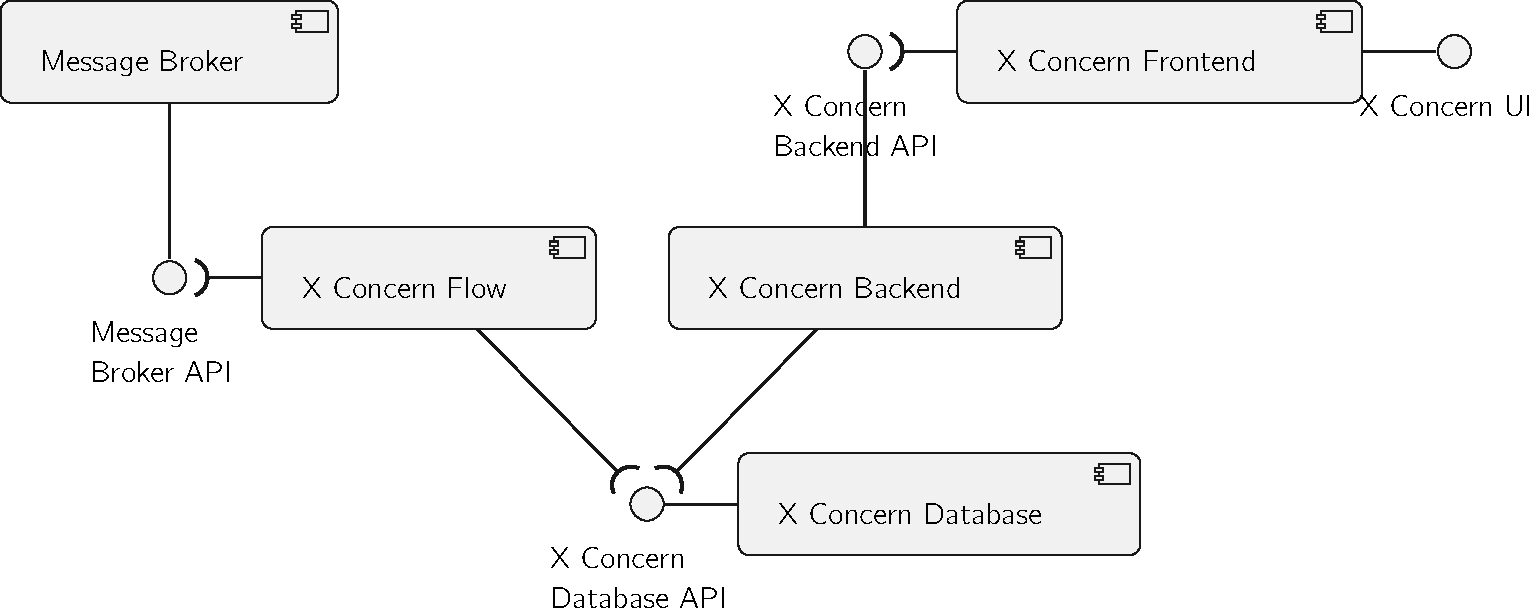
\includegraphics[page=1,width=0.8\columnwidth]{assets/diagrams/design/alternatives/internal/alternative1.pdf}
   \caption[Internal Communication - First Option - Logical View Diagram]{Internal Communication - First Option - Logical View Diagram}
   \label{fig:design:alternatives:internal:first:diagram}
\end{figure}

The approach in Figure~\ref{fig:design:alternatives:internal:first:diagram} ensures that the Message Broker is only used to transport Data Units, Alerts and Commands, alleviating it from an heavy responsibility.
That responsibility is assigned to the \textit{X Concern Flow} Container and the \textit{X Concern Database} Container.
This approach has several drawbacks such as:

\begin{itemize}
   \item The \textit{X Concern Flow} Container has full access to superfluous configuration details related to that context configuration;
   \item The same database access has to be developed and maintained in two separated containers;
   \item All database accesses are blocking calls by nature that would slow down the process;
   \item Data Flow containers can't reliably cache information collected since there is no way to know when the corresponding information was updated. Meaning that every time a new message arrives the database has to be queried.
\end{itemize}

Due to this drawbacks this option was eventually dropped.

\subsubsection{Second Option}
\label{subsubsec:design:alternatives:internal:second}

This option ensures that the Data Flow Containers are kept updated querying information from a \gls{REST} \gls{API} provided by the Configuration Containers. The logical view diagram in Figure~\ref{fig:design:alternatives:internal:second:diagram} describes how this option functions.

\begin{figure}[H]
   \centering
   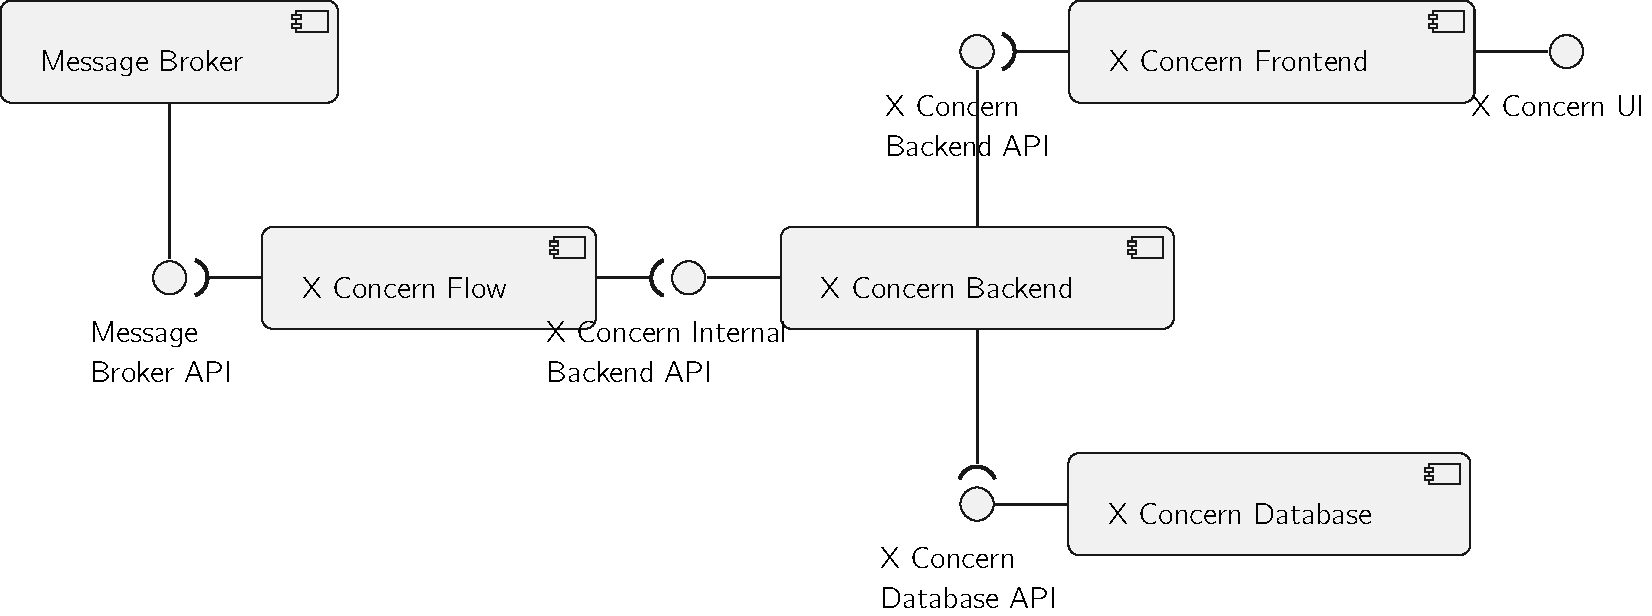
\includegraphics[page=1,width=0.8\columnwidth]{assets/diagrams/design/alternatives/internal/alternative2.pdf}
   \caption[Internal Communication - Second Option - Logical View Diagram]{Internal Communication - Second Option - Logical View Diagram}
   \label{fig:design:alternatives:internal:second:diagram}
\end{figure}

The approach in Figure~\ref{fig:design:alternatives:internal:second:diagram} doesn't suffer from all drawbacks stated for the first option but still requires a blocking call to the \textit{X Concern Backend} Container every time a new message arrives to the \textit{X Concern Flow} Container.

It's an improvement of the first option but still has some serious drawbacks and therefore it was also abandoned.

\subsubsection{Third Option}
\label{subsubsec:design:alternatives:internal:third}

This option ensures that the Data Flow Containers are kept updated by allowing them to subscribe to changes made in their concern's configuration. The logical view diagram in Figure~\ref{fig:design:alternatives:internal:third:diagram} describes how this option functions.

\begin{figure}[H]
   \centering
   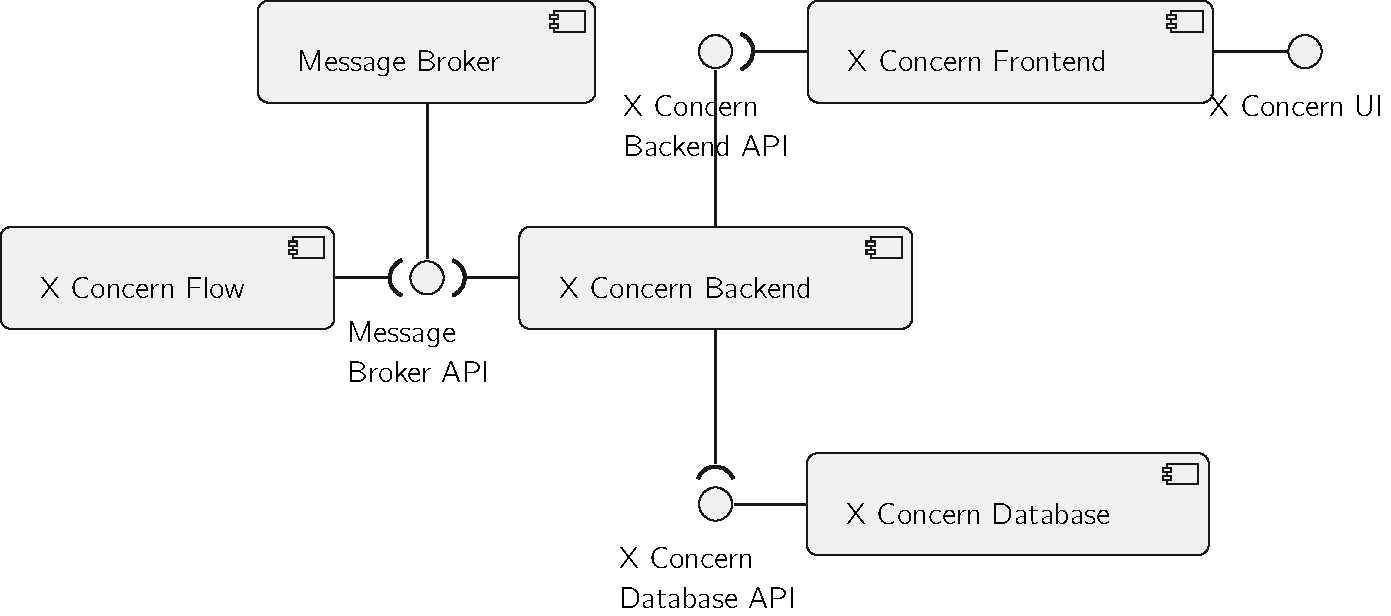
\includegraphics[page=1,width=0.8\columnwidth]{assets/diagrams/design/alternatives/internal/alternative3.pdf}
   \caption[Internal Communication - Third Option - Logical View Diagram]{Internal Communication - Third Option - Logical View Diagram}
   \label{fig:design:alternatives:internal:third:diagram}
\end{figure}

The major improvement of the approach in Figure~\ref{fig:design:alternatives:internal:third:diagram} when compared with the options above is that, since \textit{X Concern Flow} Container subscribes to configuration updates, it can reliably keep a cache with just the needed information (and not the entire concern configuration). This works since \textit{X Concern Flow} Containers can discard updates related to information that they currently don't use. Once the container needs that information, it can send an event requesting what it needs and that information arrives later as a normal update to the configuration.
All \textit{X Concern Flow} external interactions also rely on asynchronous communication, ensuring a more robust performance.

The main drawback to this option is that the \textit{Message Broker} becomes responsible for yet another communication topic inside the environment.

Despite this drawback this is the option currently in use. The following options purpose alternatives to tackle this drawback.

\subsubsection{Fourth Option}
\label{subsubsec:design:alternatives:internal:fourth}

This option ensures that the Data Flow Containers are kept updated by allowing them to query information from an \textit{Internal State Database}. This approach differs from the first option since the \textit{Internal State Database} is supposed to be a fast in memory database with only the needed information for Data Flow Containers to process Data Units, Alerts and Commands. The logical view diagram in Figure~\ref{fig:design:alternatives:internal:fourth:diagram} describes how this option functions.

\begin{figure}[H]
   \centering
   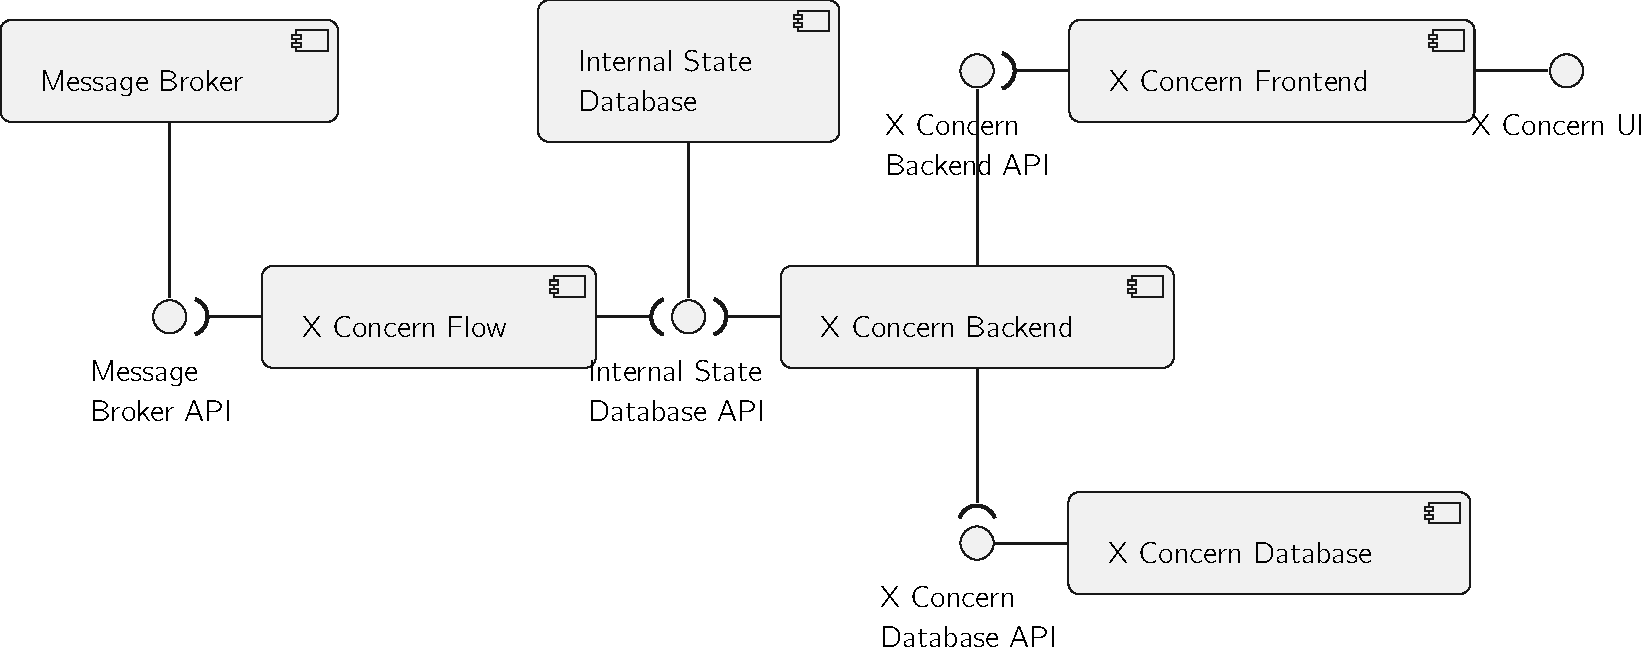
\includegraphics[page=1,width=0.8\columnwidth]{assets/diagrams/design/alternatives/internal/alternative4.pdf}
   \caption[Internal Communication - Fourth Option - Logical View Diagram]{Internal Communication - Fourth Option - Logical View Diagram}
   \label{fig:design:alternatives:internal:fourth:diagram}
\end{figure}

The approach in Figure~\ref{fig:design:alternatives:internal:fourth:diagram} would remove the responsibly from the \textit{Message Broker} to maintaining the internal state updated in the Data Flow Scope.
The \textit{Internal State Database} would in turn store information that \textit{X Content Flow} could query.

The main drawbacks of this approach are the same stated in the second option, even tho they can be mitigated by leveraging technologies that tackle distributed caching problems.

\subsubsection{Fifth Option}
\label{subsubsec:design:alternatives:internal:fifth}

This option ensures that the Data Flow Containers are kept updated by allowing them to subscribe to changes made in their concern's configuration. This option diverges from the third option since the event store would persist all updates to concerns configurations. The logical view diagram in Figure~\ref{fig:design:alternatives:internal:fifth:diagram} describes how this option functions.

\begin{figure}[H]
   \centering
   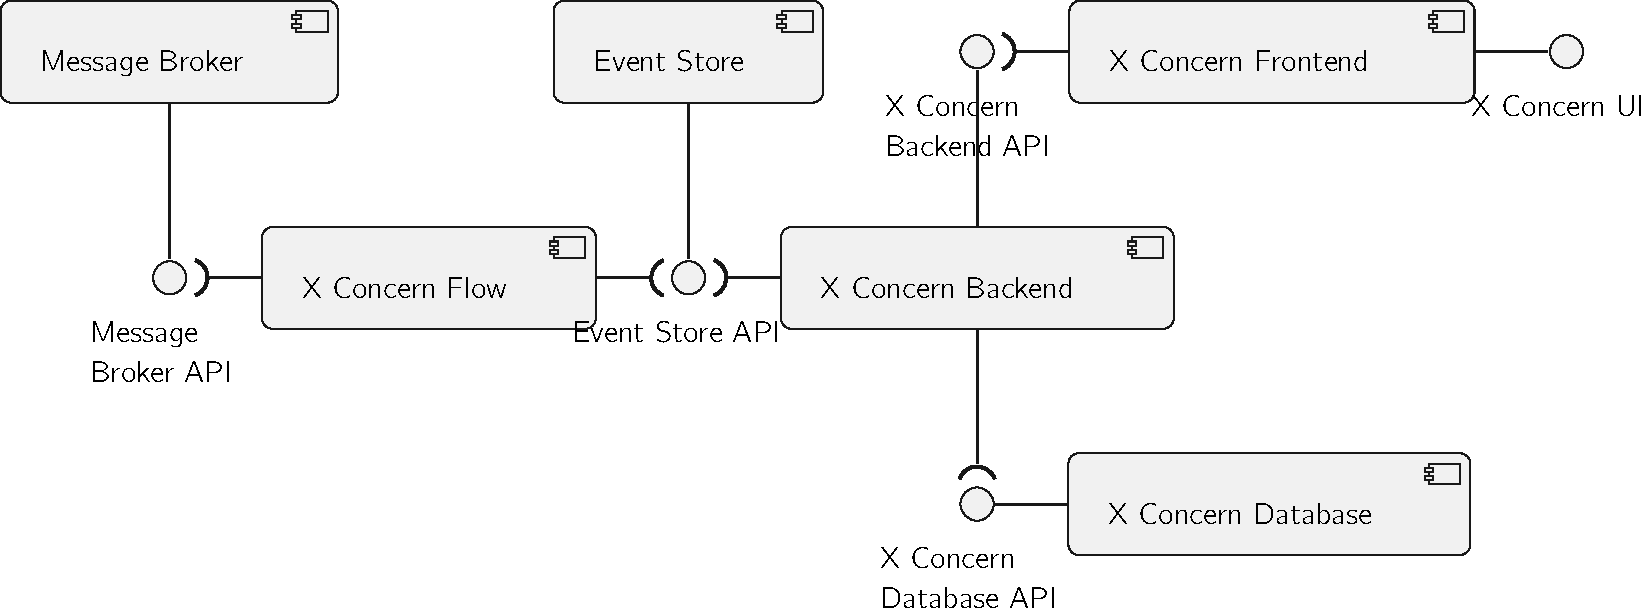
\includegraphics[page=1,width=0.8\columnwidth]{assets/diagrams/design/alternatives/internal/alternative5.pdf}
   \caption[Internal Communication - Fifth Option - Logical View Diagram]{Internal Communication - Fifth Option - Logical View Diagram}
   \label{fig:design:alternatives:internal:fifth:diagram}
\end{figure}

The \textit{X Concern Flow} Container would use event sourcing to reach the current state of its concern configuration on start up and then cache this state internally. New events would then be sent automatically via subscription to keep the state up-to-date.

The main drawback of the approach in Figure~\ref{fig:design:alternatives:internal:fifth:diagram} is that the container can't keep just the needed portion of configurations without recreating the entire state though event sourcing.

\subsection{Synopsis}
\label{subsubsec:design:alternatives:synopsis}

This section presented the most important architectural decisions that lead to this project's solution, \textbf{Sensae Console}. The next section presents the architectural design of the developed \textbf{Business Applications}.

\section{Business Applications - Architectural Design}
\label{subsec:design:architecture:solutions}

This section will explore the details of each Business Application developed as a \gls{PoC} from an architectural point of view.
The description will follow the same methodology of the \nameref{sec:design:architecture} Section.
Most concepts regarding the C4 Level 1 - Context were already described in Section~\ref{subsec:design:architecture:context}, therefore this section focus on the C4 Level 2 - Container.
Some of the similarities shared between the architecture of all services are:

\begin{itemize}
   \item All include a backend that exposes an \gls{API};
   \item All include a frontend that exposes a \gls{UI};
   \item All include at least a database that exposes an \gls{API} consumed solely by the service's backend;
   \item Any communication with \textbf{Sensae Console} is preformed by consuming the Message Broker's \gls{API};
   \item All follow the idea behind the separation of responsibilities seen in a three layer architecture.
\end{itemize}

Even though it isn't required, the \textbf{UI Aggregator} can be configured to consume the \gls{UI} and \gls{API} belonging to each Business Application. By doing so, the complete solution, \gls{UI} and \gls{API} can be presented under a single \gls{FQDN}. This view can be seen in Appendix~\ref{AppendixB}.

For brevity reasons the C4 level 3 of the solutions will not be discussed, the architecture of most containers follows what was discussed in Appendix~\ref{appendix:design:architecture:platform:components} Section. The frontend containers behave exactly as the ones designed for the platform and most backend containers follow the same ideas behind the Configuration Backend Architecture for containers in the platform. The architectures that diverge a bit can be consulted in Appendix~\ref{AppendixC2}.

\subsection{Fleet Management}
\label{subsubsec:design:architecture:solutions:fleet}

The logical view of the Fleet Management service is presented in Figure~\ref{fig:design:architecture:solutions:containers:logical:fleet}.

This service is composed by a simple three layers architecture. The details related to this service are discussed in Section~\ref{subsubsec:design:domain:bounded_contexts:fleet}.

\begin{figure}[H]
   \centering
   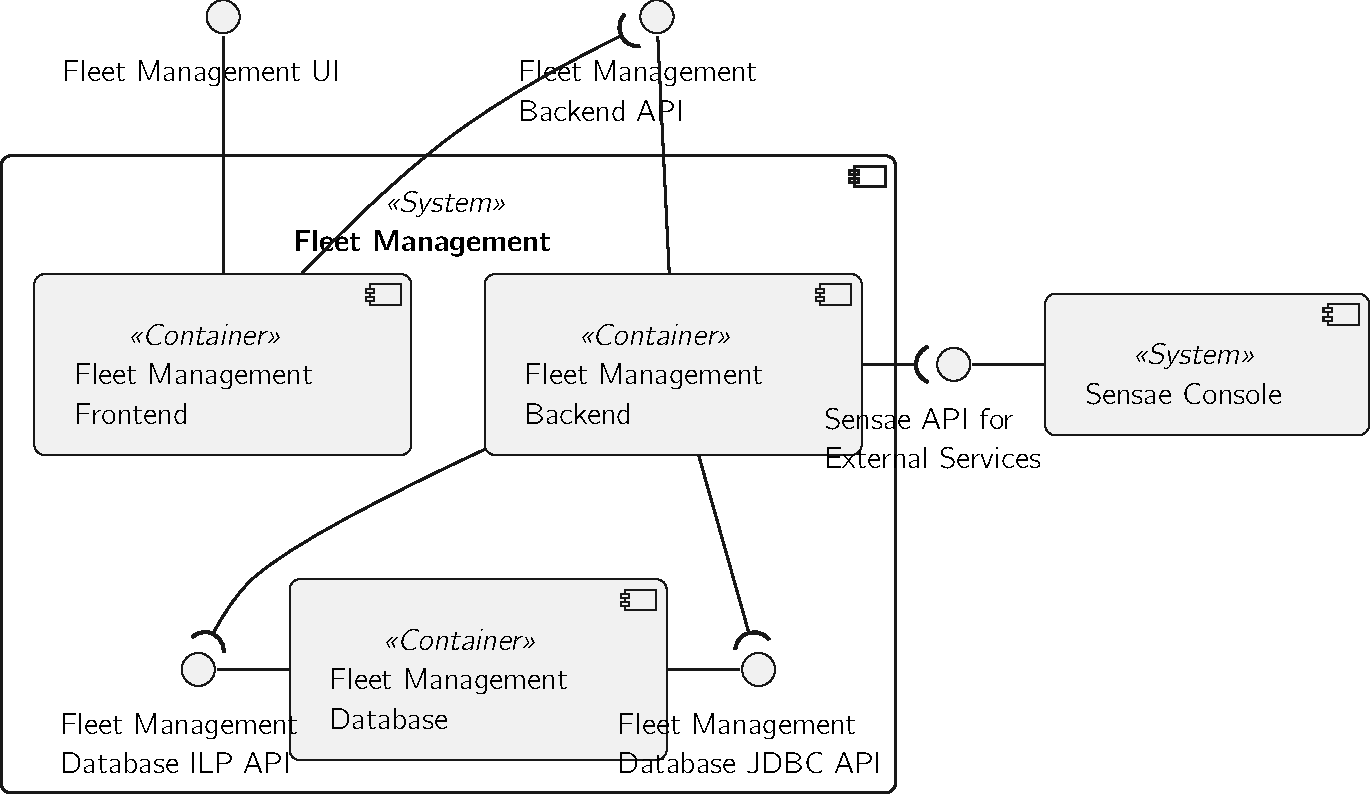
\includegraphics[page=1,width=0.75\columnwidth]{assets/diagrams/design/architectural/level2/logical/fleet-management-context.pdf}
   \caption[Fleet Management - Container Level - Logical View Diagram]{Fleet Management - Container Level - Logical View Diagram}
   \label{fig:design:architecture:solutions:containers:logical:fleet}
\end{figure}

Next, to better understand the internal processes of this service, Figure~\ref{fig:design:architecture:container:process:diagram:fleet} presents how a user can see the current location of a device. Authentication details are omitted for brevity reasons.

In order to provide live information to the user, the Fleet Management service (and all other \textbf{Business Applications}) relies on \textit{WebSockets}. As seen in Figure~\ref{fig:design:architecture:container:process:diagram:fleet} a bidirectional channel is created between the frontend and backend so that data can be sent directly from the backend to the frontend as we can see in the step \textbf{2.5}. Fist the frontend must subscribe to new information with a valid \textit{access token} - steps \textbf{1.2} to \textbf{1.6} - then this channel is maintained till the user leaves the page. Once the user leaves the page the subscription is closed in the frontend and subsequently in the backend - steps \textbf{3.2} to \textbf{3.5}.

\begin{figure}[H]
   \centering
   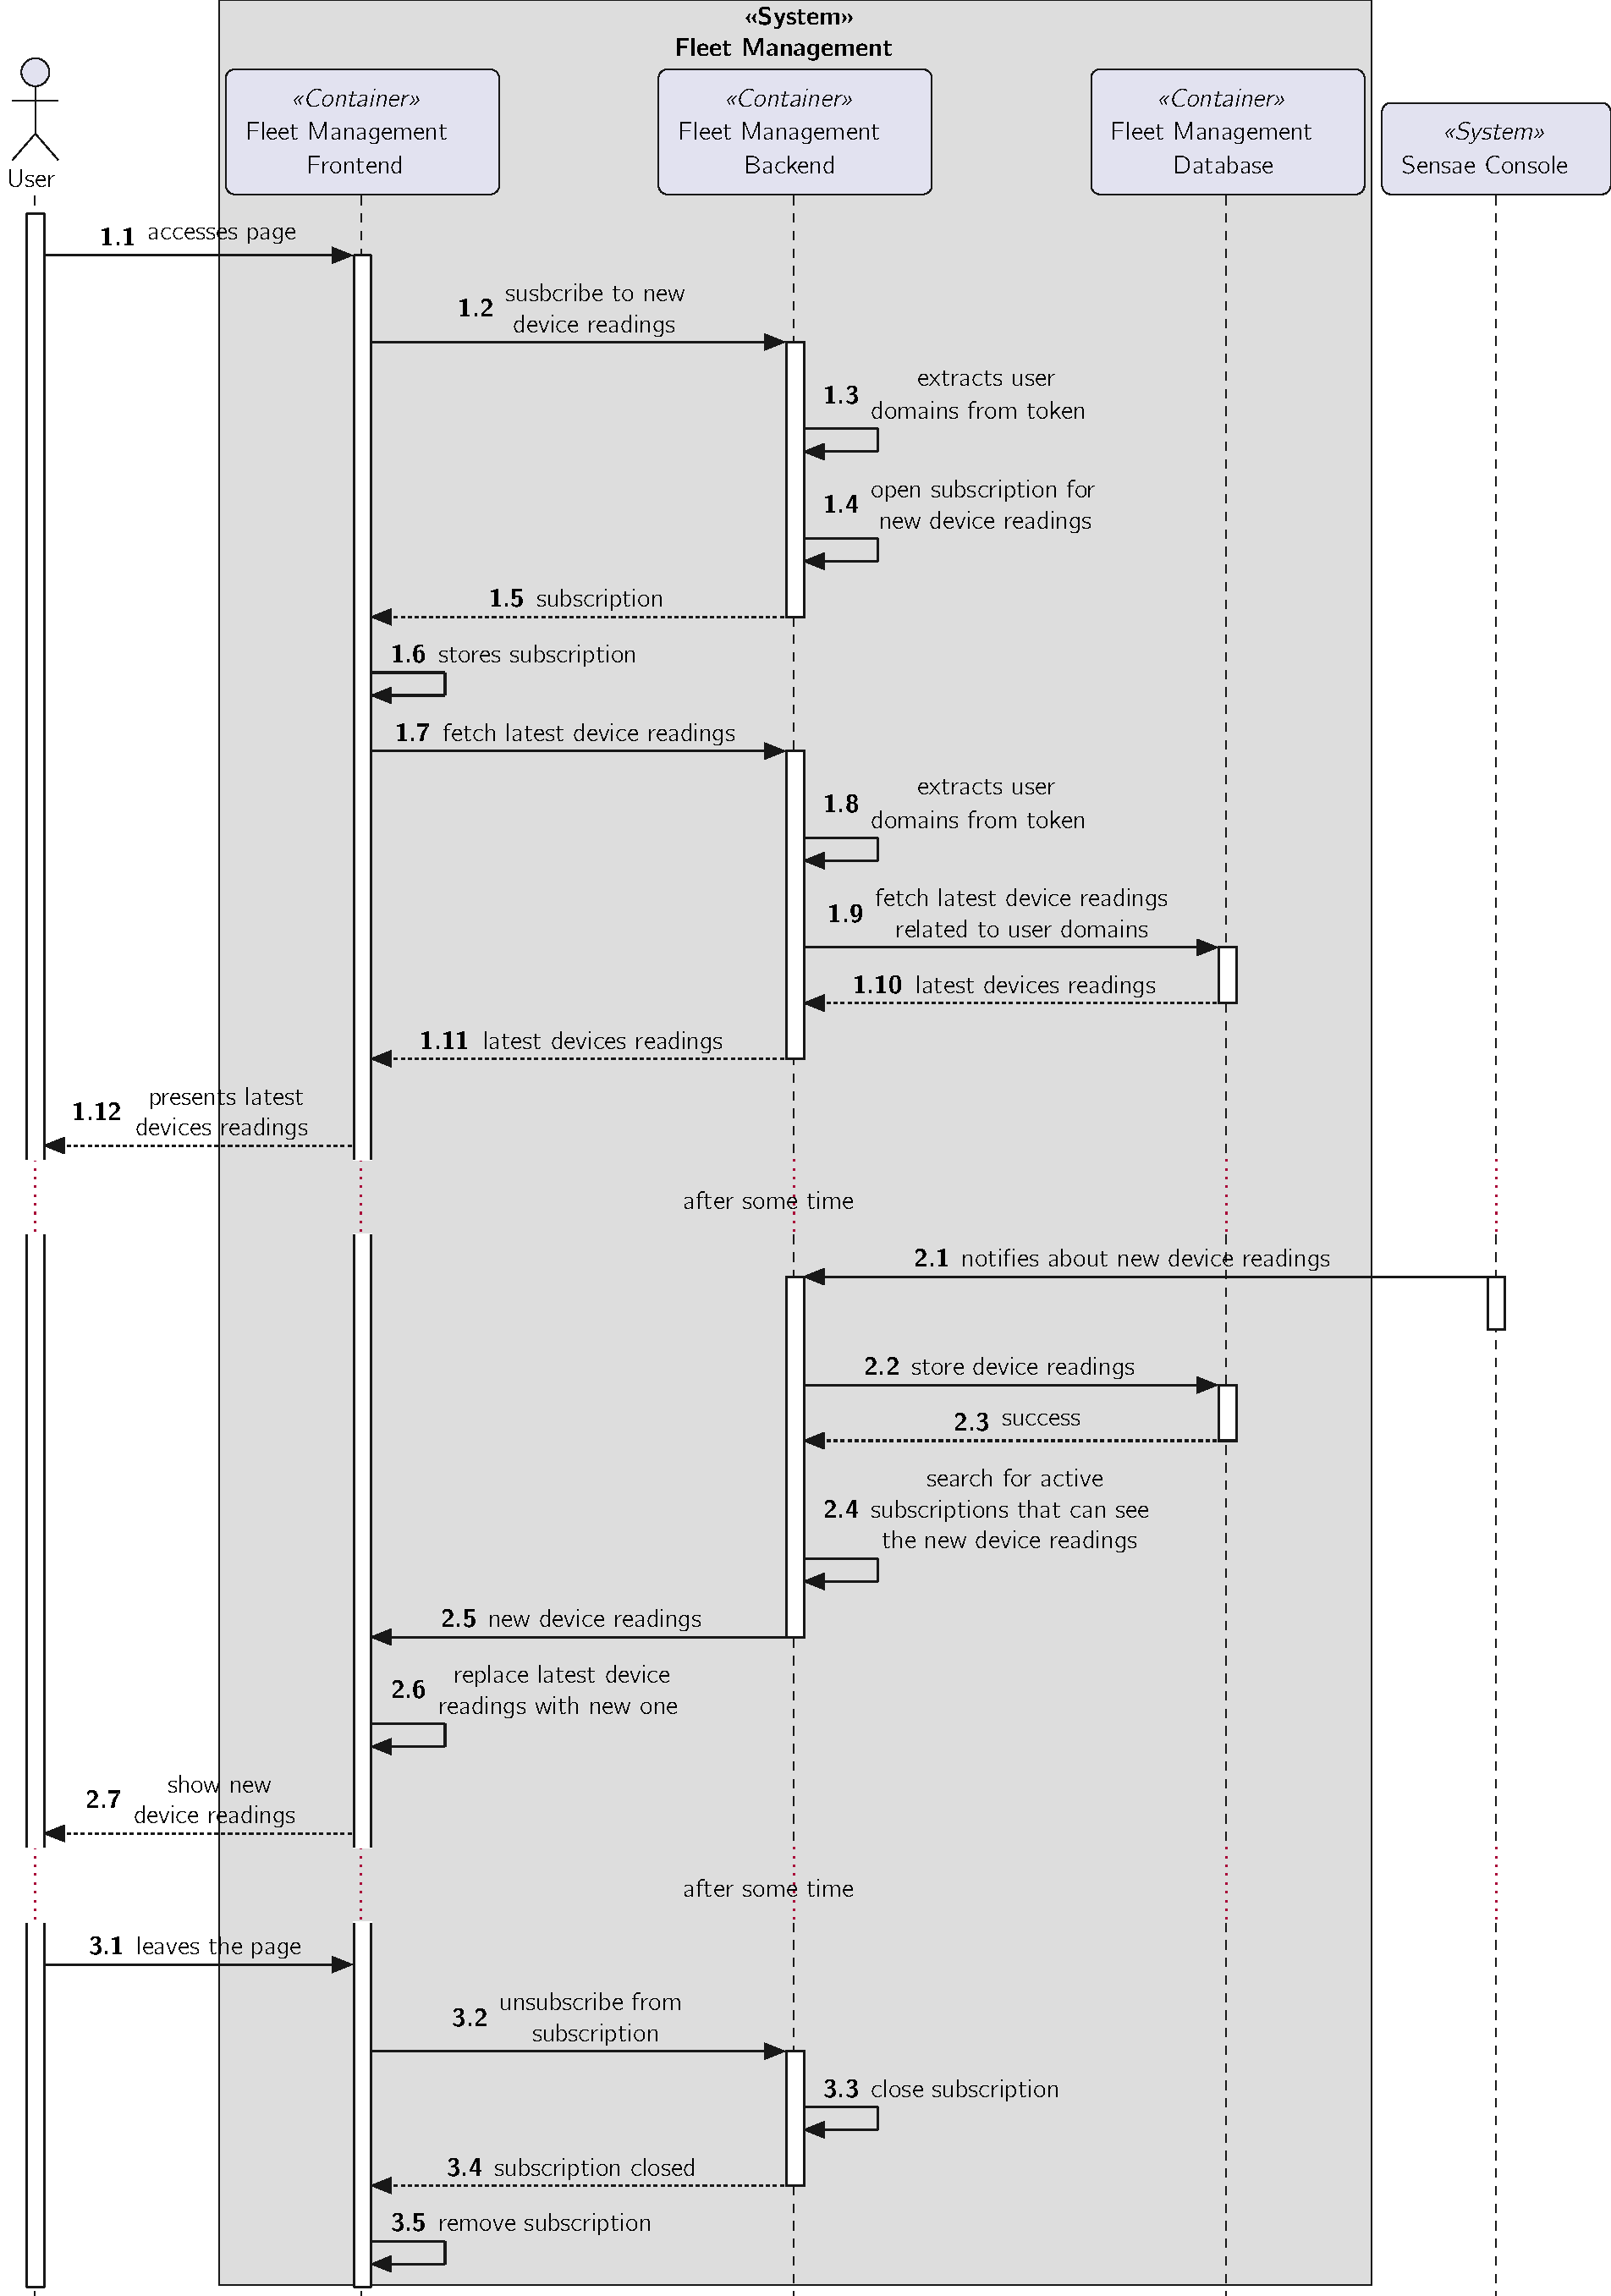
\includegraphics[page=1,width=\columnwidth]{assets/diagrams/design/architectural/level2/process/device-live-location.pdf}
   \caption[Consult Device Live Location - Container Level - Process View Diagram]{Consult Device Live Location - Container Level - Process View Diagram}
   \label{fig:design:architecture:container:process:diagram:fleet}
\end{figure}

\subsection{Notification Management}
\label{subsubsec:design:architecture:solutions:notification}

The logical view of Notification Management service is presented in Figure~\ref{fig:design:architecture:solutions:containers:logical:noti}.

\begin{figure}[H]
   \centering
   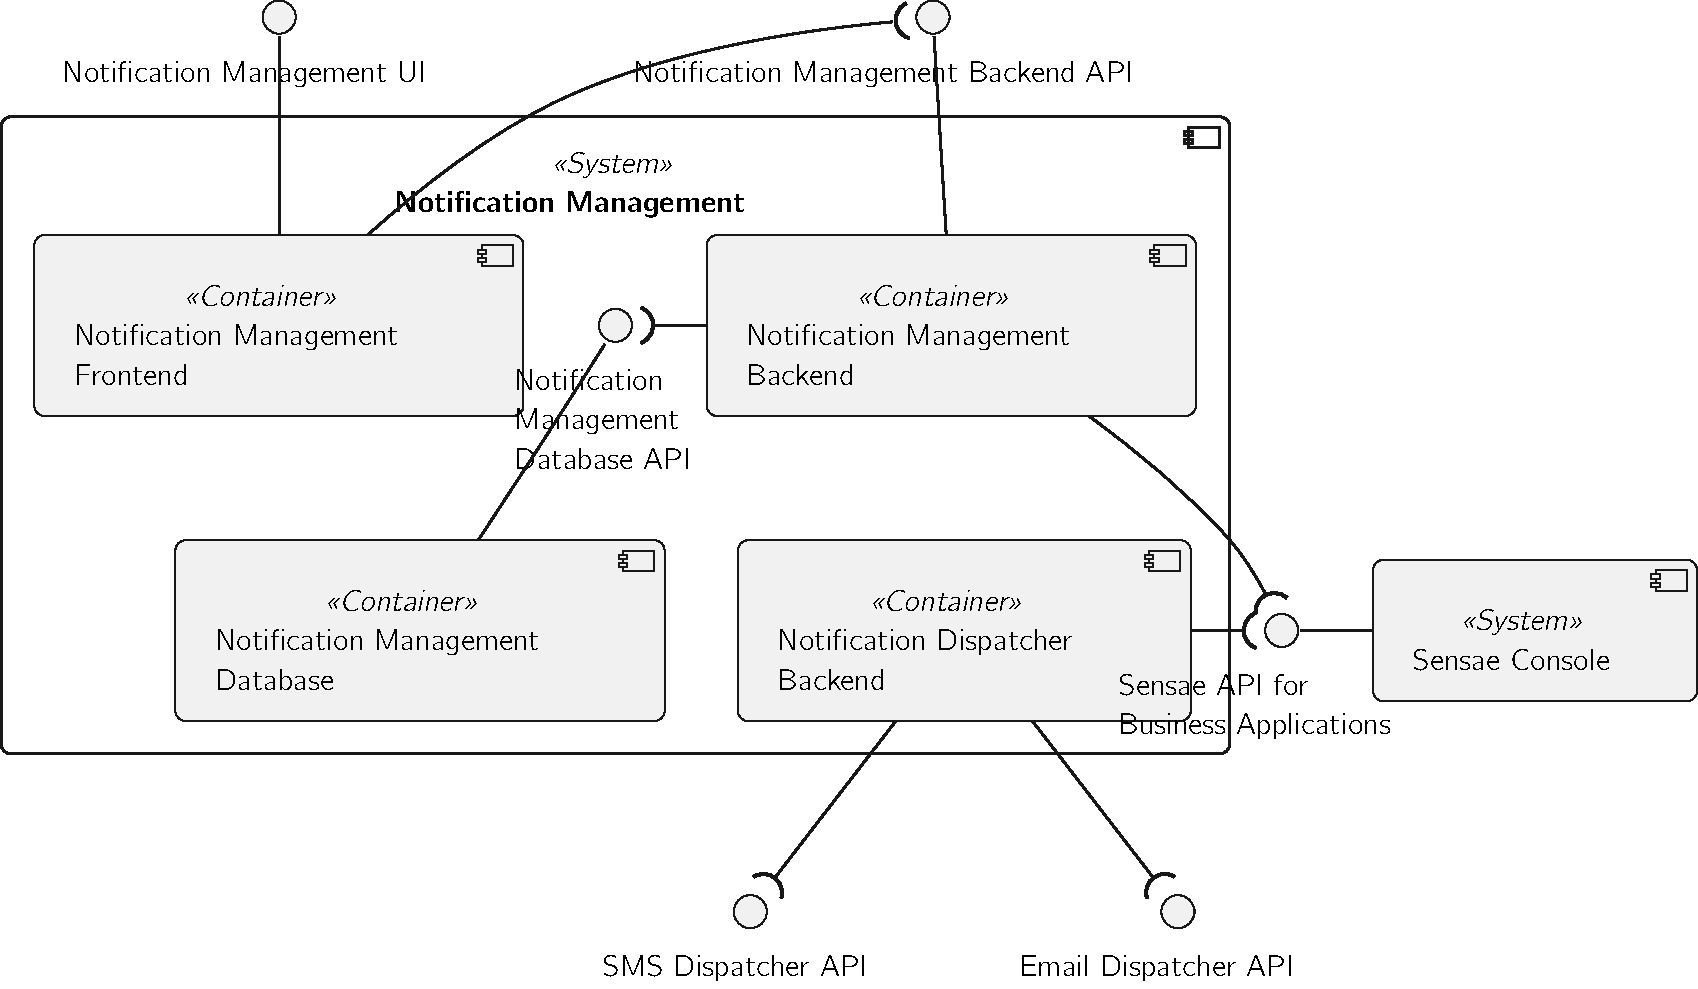
\includegraphics[page=1,width=0.8\columnwidth]{assets/diagrams/design/architectural/level2/logical/notification-management-context.pdf}
   \caption[Notification Management - Container Level - Logical View Diagram]{Notification Management - Container Level - Logical View Diagram}
   \label{fig:design:architecture:solutions:containers:logical:noti}
\end{figure}

This service is composed by a simple three layers architecture and has a separated container responsible for dispatching SMS and emails, the Notification Dispatcher Backend container. Information regarding the type of alerts each user is interested in are exchanged between the Backend and Dispatcher containers through the Message Broker. The details related to this service are discussed in Section~\ref{subsubsec:design:domain:bounded_contexts:notification}.

The next diagram in Figure~\ref{fig:design:architecture:container:process:diagram:notification} describes how a user receives notifications via several different delivery channels. For brevity reasons the subscription process is omitted.

As a brief description the diagram in Figure~\ref{fig:design:architecture:container:process:diagram:notification} describes what happens when an alert is dispatched inside \textbf{Sensae Console}. An alert is created in Alert Dispatcher Backend, flows though Device Ownership Backend to be enriched with the domains that own it and is then collected by, at least, the Notification Management Service. Notification Management Backend deliveries alerts in the form of \gls{UI} notifications - step \textbf{2.5} and \textbf{2.6} - and stores this alert as a notification for later use - step \textbf{2.3}. Notification Dispatcher Backend deliveries alerts in the form of Emails - step \textbf{3.4} - and SMS - step \textbf{3.7}.

\begin{figure}[H]
   \centering
   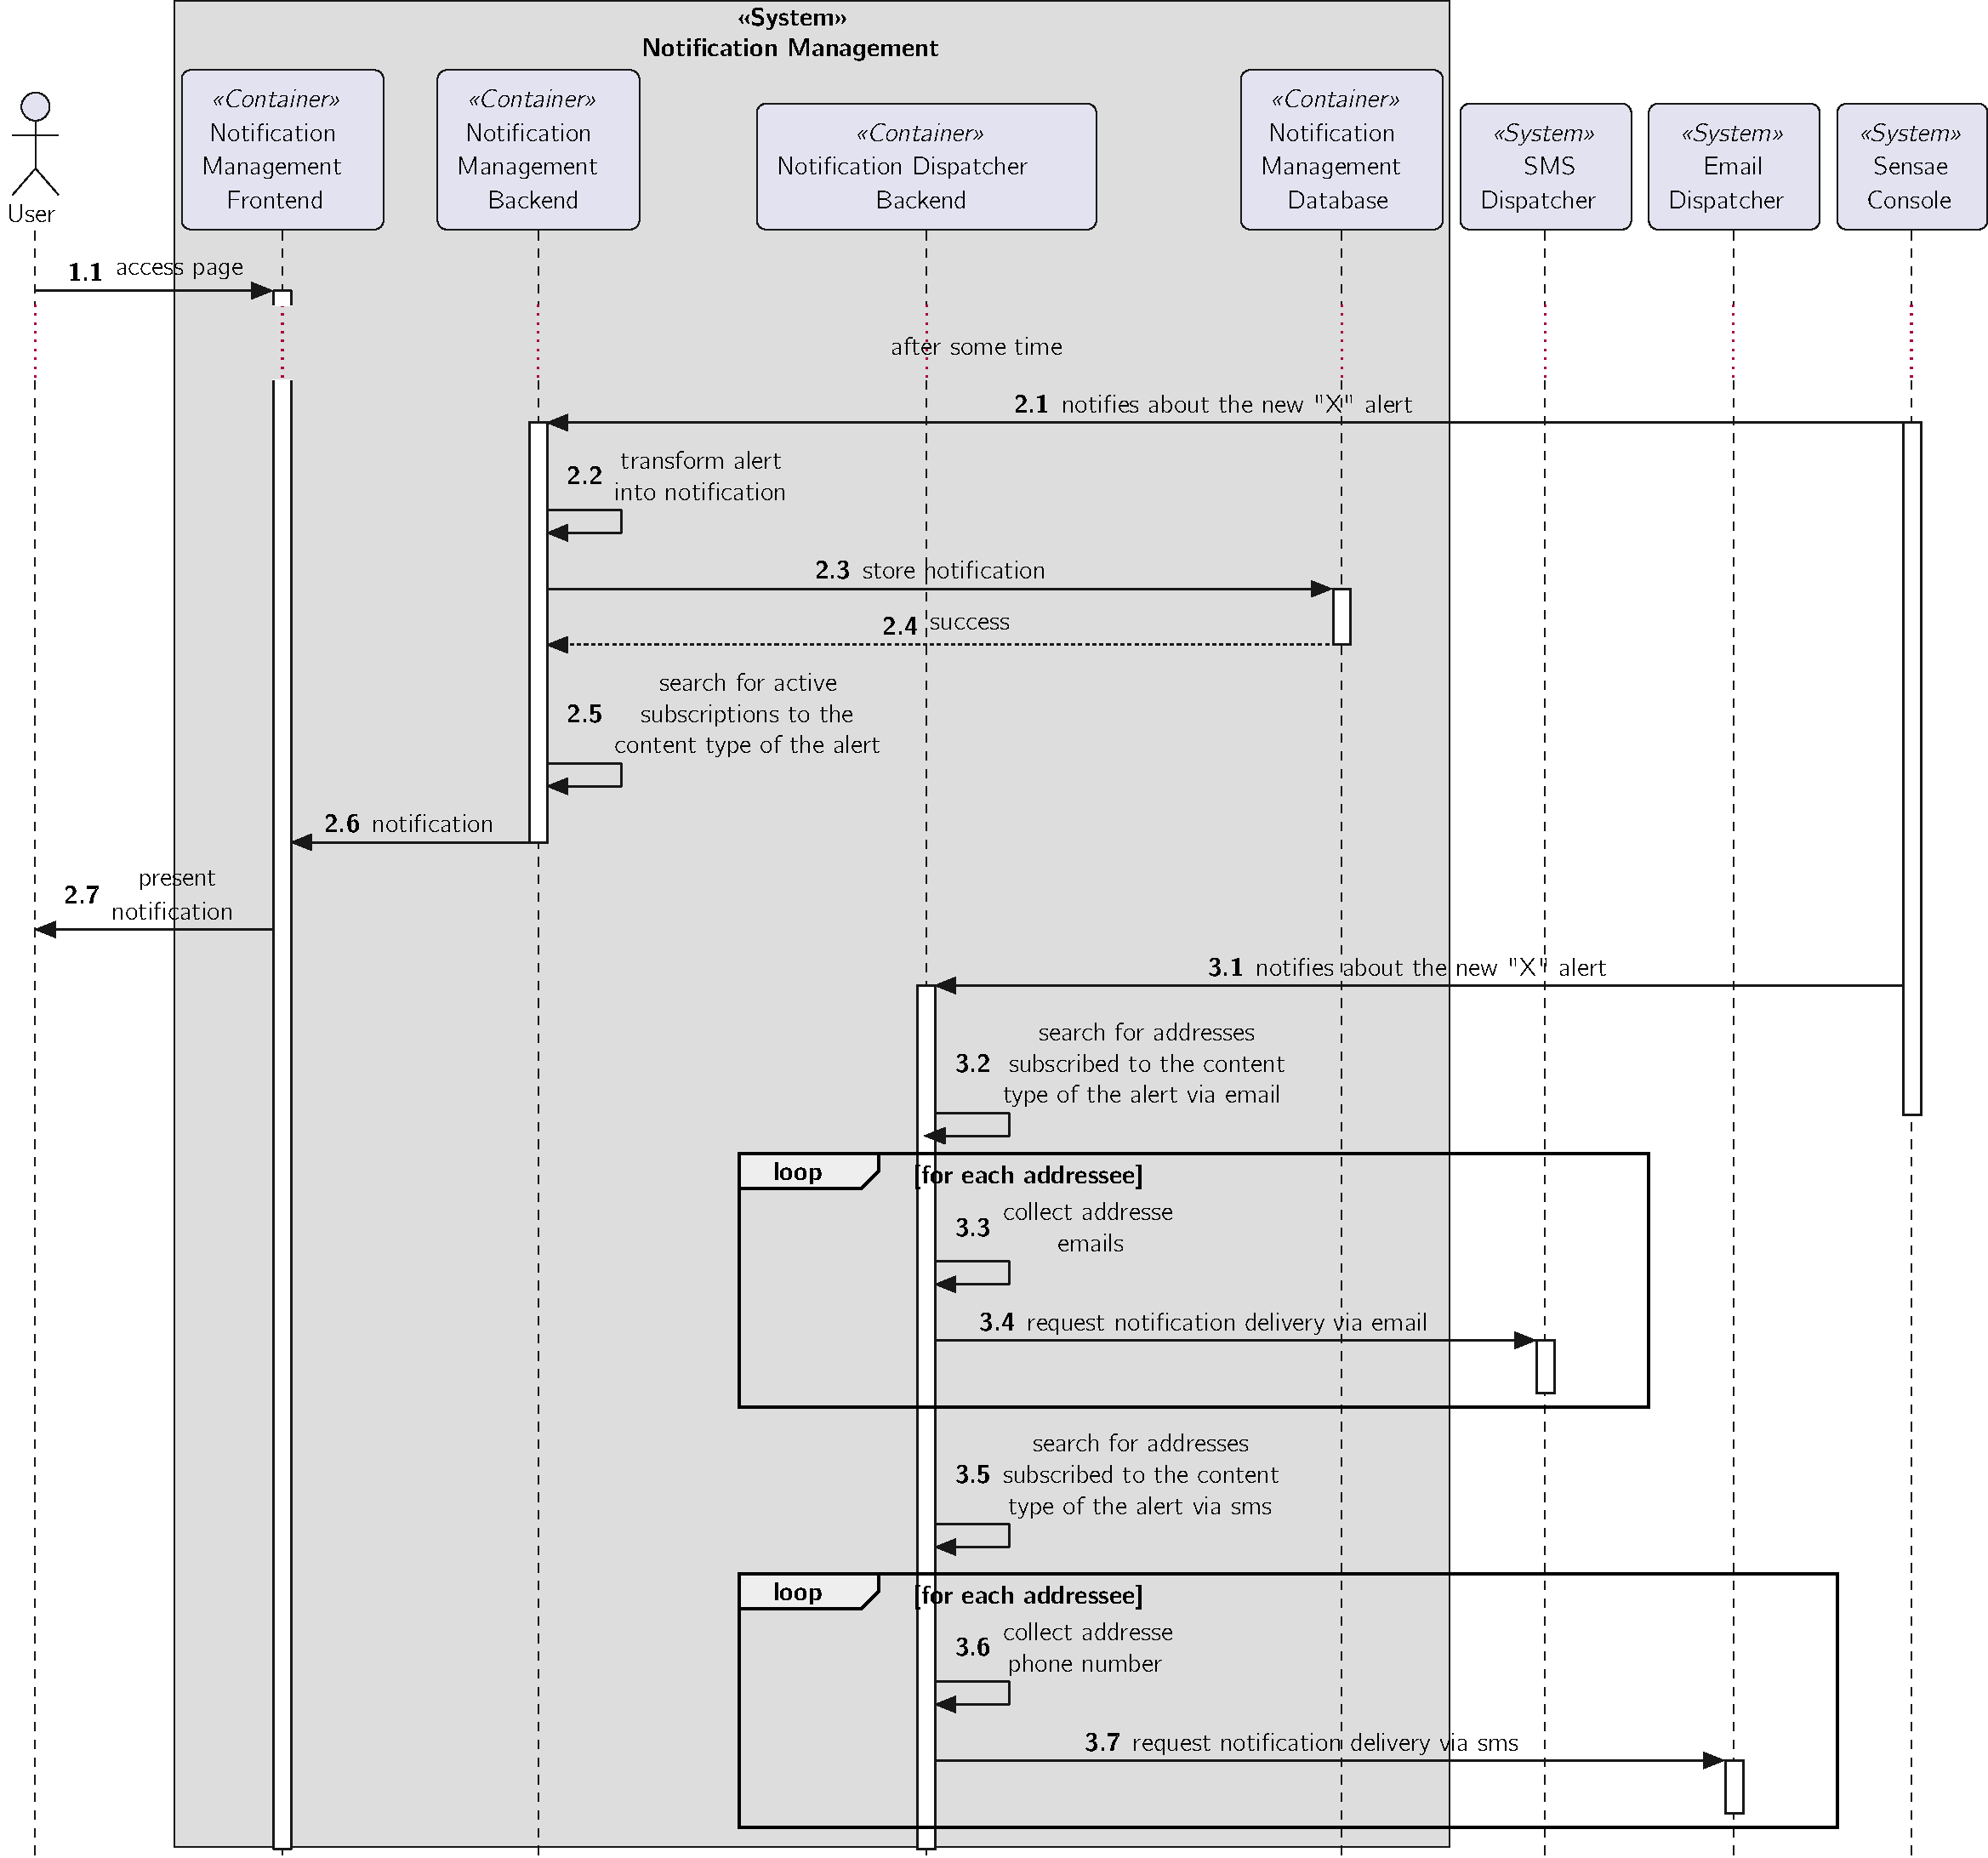
\includegraphics[page=1,width=\columnwidth]{assets/diagrams/design/architectural/level2/process/notification-dispatch.pdf}
   \caption[Receive Notification - Container Level - Process View Diagram]{Receive Notification - Container Level - Process View Diagram}
   \label{fig:design:architecture:container:process:diagram:notification}
\end{figure}

\subsection{Smart Irrigation}
\label{subsubsec:design:architecture:solutions:irrigation}

The logical view of the Smart Irrigation service is presented in Figure~\ref{fig:design:architecture:solutions:containers:logical:irrigation}.

This service is composed by a three layers architecture, the \textbf{Data Layer} is divided in two databases, one responsible for storing device measures and another responsible for storing information regarding the Irrigation Zones and device information. The details related to this service are discussed in Section~\ref{subsubsec:design:domain:bounded_contexts:irrigation}.

Certain types of alerts are also collected by Smart Irrigation Backend to automatically control conditions inside an irrigation zone. The diagram in Figure \ref{fig:design:architecture:container:process:diagram:irrigation} presents this process.

\begin{figure}[H]
   \centering
   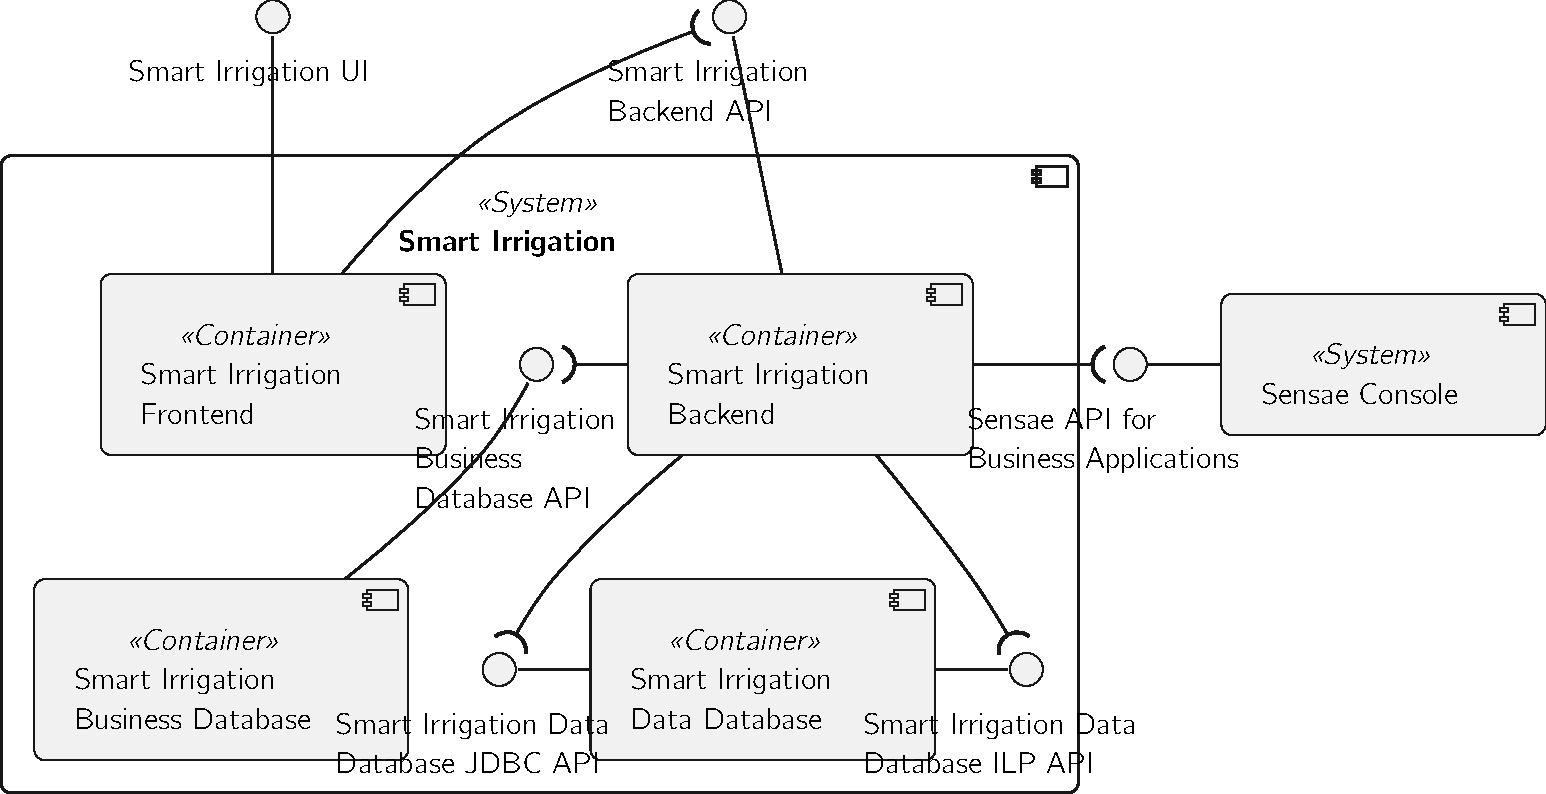
\includegraphics[page=1,width=0.75\columnwidth]{assets/diagrams/design/architectural/level2/logical/smart-irrigation-context.pdf}
   \caption[Smart Irrigation - Container Level - Logical View Diagram]{Smart Irrigation - Container Level - Logical View Diagram}
   \label{fig:design:architecture:solutions:containers:logical:irrigation}
\end{figure}

\begin{figure}[H]
   \centering
   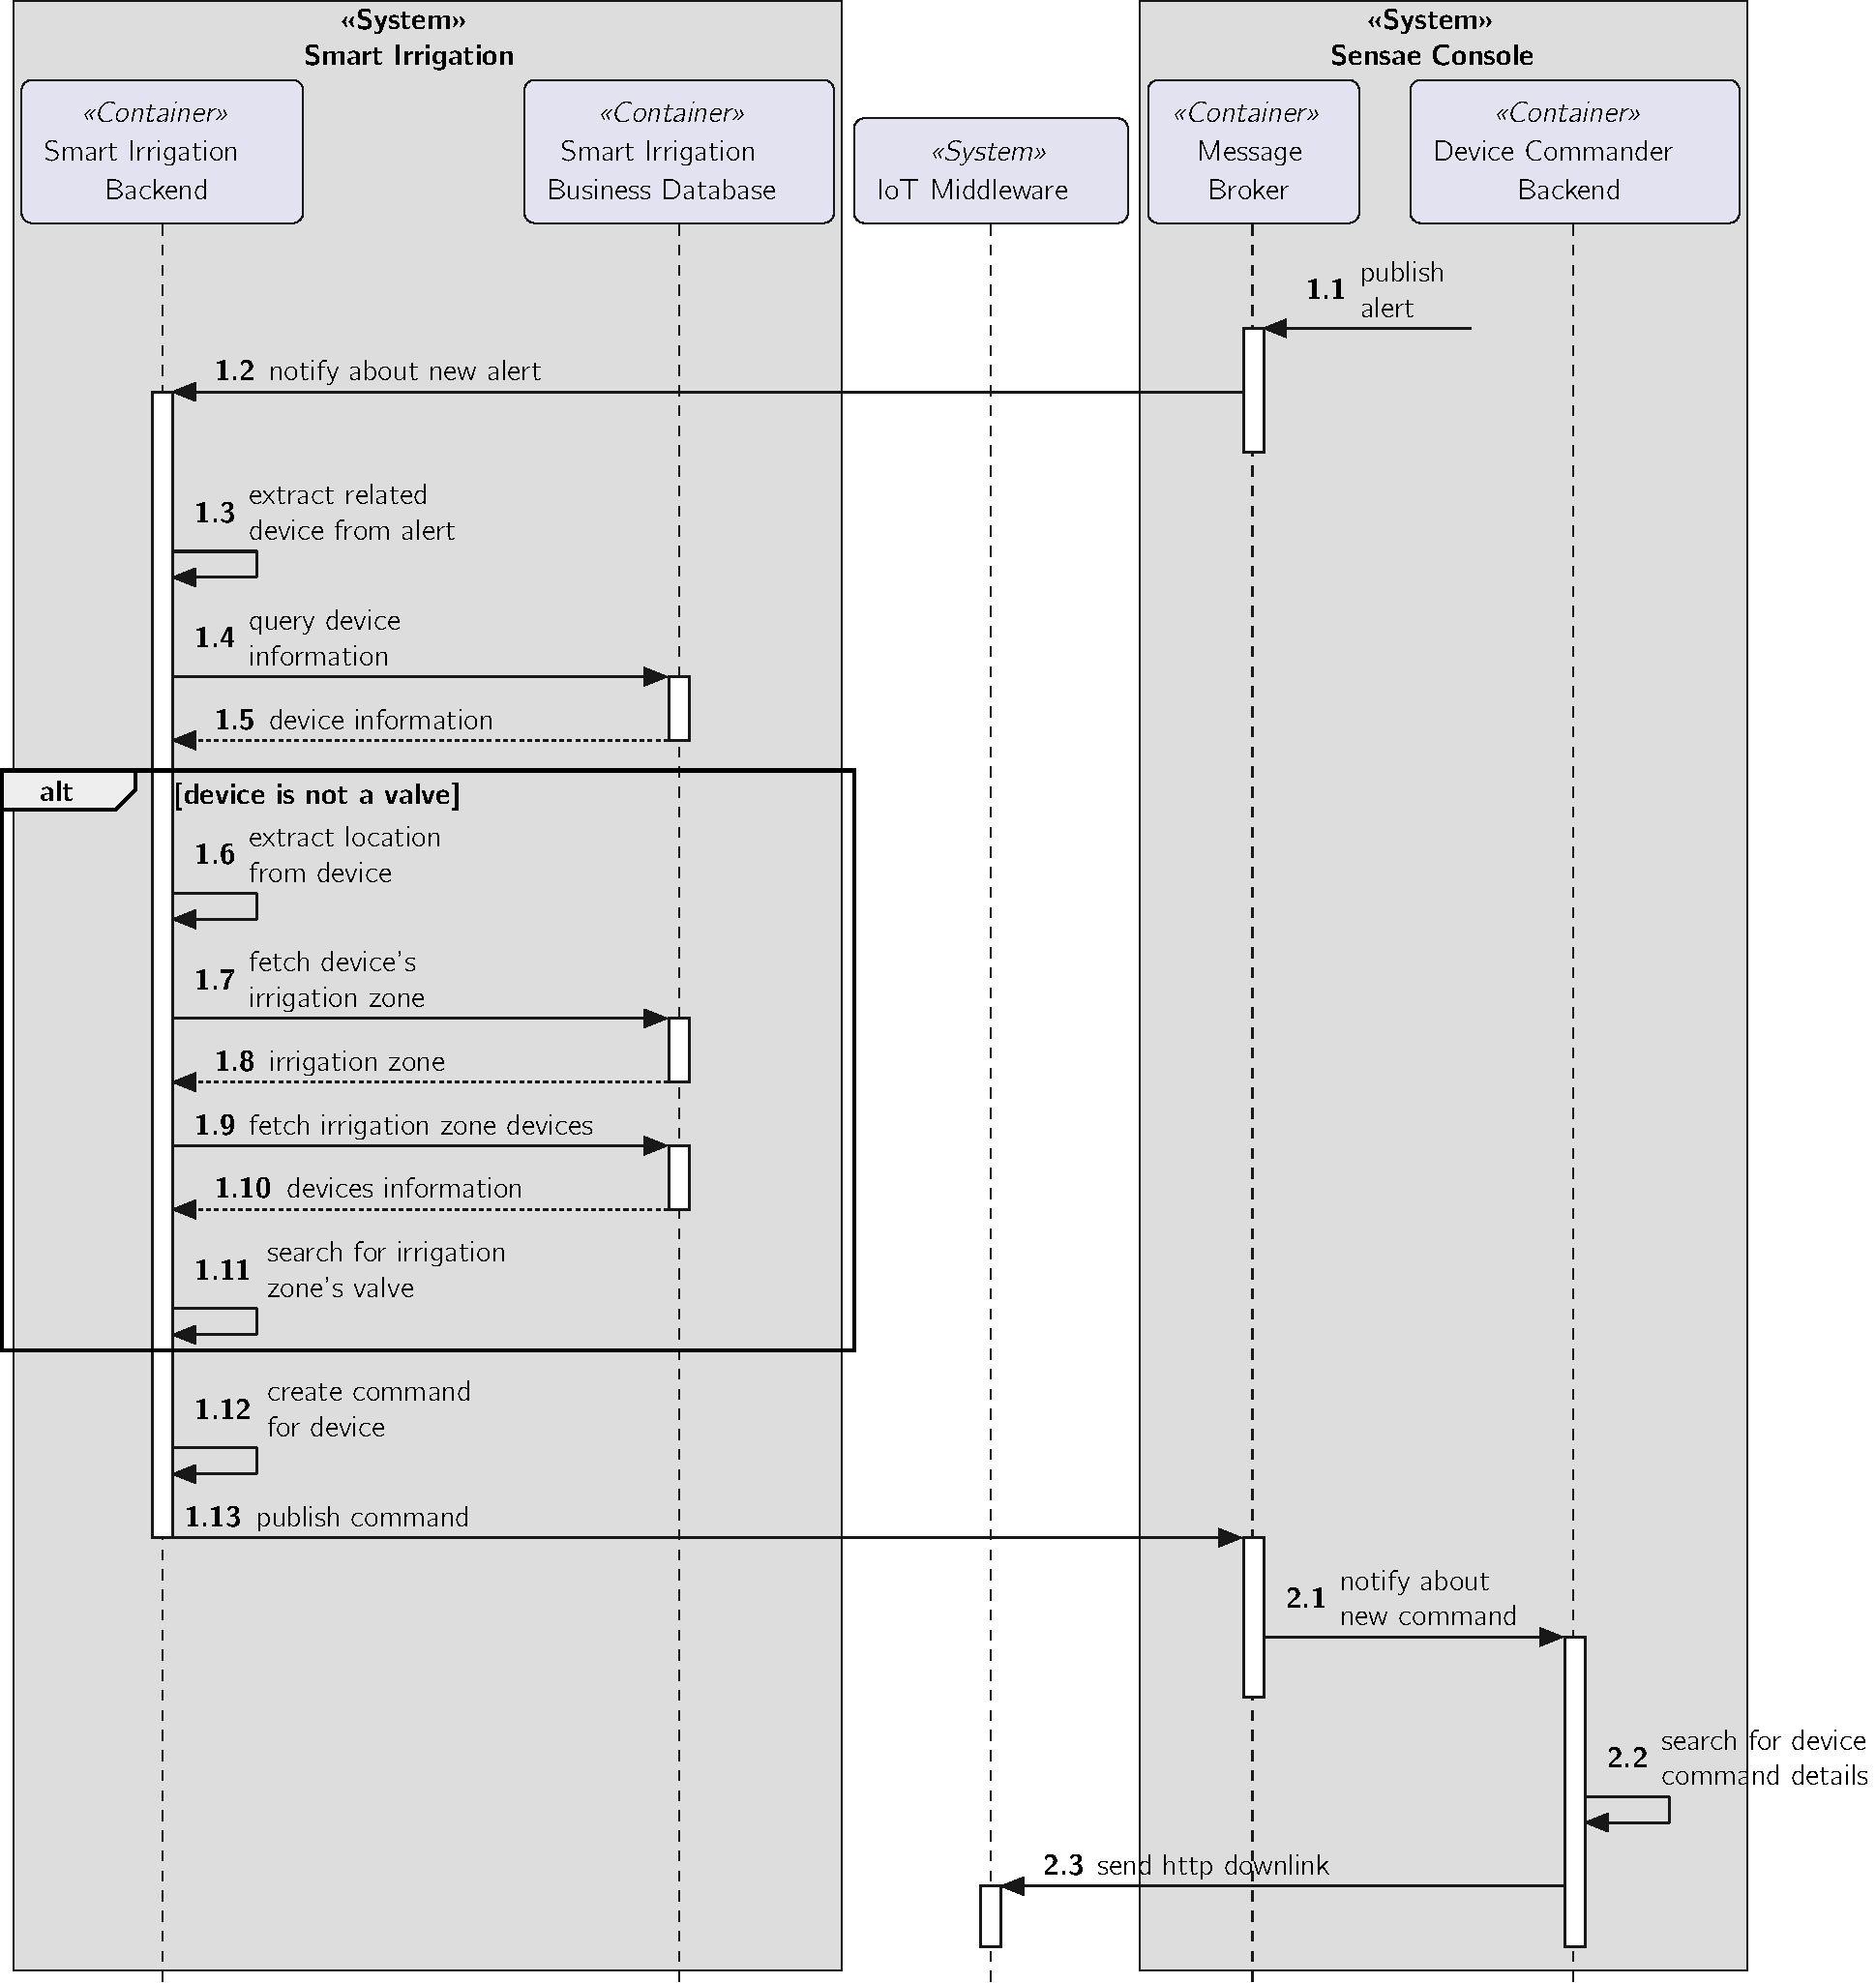
\includegraphics[page=1,width=0.9\columnwidth]{assets/diagrams/design/architectural/level2/process/smart-irrigation.pdf}
   \caption[Valve Activation Process - Container Level - Process View Diagram]{Valve Activation - Container Level - Process View Diagram}
   \label{fig:design:architecture:container:process:diagram:irrigation}
\end{figure}

The alerts created in \textbf{Sensae Console} are captured by \textbf{Business Applications}'s containers so that they can immediately act based on those alerts (Figure~\ref{fig:design:architecture:container:process:diagram:irrigation}).

The Smart Irrigation Backend subscribes to three types of \textit{Sub Category} alerts, all with the same \textit{Category} - \textit{Smart Irrigation}:

\begin{itemize}
   \item \textbf{Damped Environment}: a valve needs to be closed;
   \item \textbf{Dry Environment}: a valve needs to be open;
   \item \textbf{Valve Open For Lengthy Period}: a valve needs to be close.
\end{itemize}

\section{Synopsis}
\label{sec:design:synopsis}

This chapter presented the design of the platform, \textbf{Sensae Console}, and the solutions, \textbf{Business Applications}. Topics such as the domain, the architectural design and alternatives have been discussed here. To complement the description of the system, the next chapter introduces how, following the design proposed, this whole solution was implemented.
